\documentclass[twocolumn]{article}

\usepackage{wasysym} % for male and female symbols

\usepackage[utf8]{inputenc} % Ensures UTF-8 encoding for special characters
\usepackage[ngerman]{babel} % Adapts language elements (e.g., "Abbildung" instead of "Figure") to German

% Formatting and Layout
\usepackage{geometry} % Adjusts page margins and layout
\usepackage{tcolorbox} % Creates colored boxes for emphasis or notes
\usepackage{mdframed} % Allows framed environments with background colors
\usepackage{multicol} % switch between single and two columns

% Math and Symbols
\usepackage{amsmath} % Provides advanced mathematical typesetting

% Tables and Colors
\usepackage{booktabs} % Enhances table formatting for professional appearance
\usepackage{graphicx} % Enables the inclusion of images
\usepackage[table,xcdraw]{xcolor} % Adds colors to tables and drawings

% Listings and Code
\usepackage{listings} % Formats code listings in a basic way
\usepackage{minted} % Formats code listings with syntax highlighting (requires Pygments)

% Text Manipulation
\usepackage{soul} % Allows text highlighting, strikethrough, etc.
\usepackage{emoji} % Enables inserting emojis into the document

% Lists and Enumerations
\usepackage{enumitem} % Allows me to make smore compact lists

% Figures and Captions
\usepackage{subcaption} % Supports subfigures with individual captions

% External Content and Hyperlinks
\usepackage{pdfpages} % Includes external PDFs in the document
\usepackage{hyperref} % Enables clickable links and \url command

% Miscellaneous
\usepackage{jupynotex} % For integrating Jupyter Notebook outputs into LaTeX

\geometry{
 a4paper,
 total={170mm,257mm},
 left=25mm,
 top=20mm,
 }

\newcommand\todo[1]{\noindent\textcolor{orange}{\emoji{warning} #1}}
\newcommand{\singleslide}[1]{
    \begin{tcolorbox}[colframe=black!75, width=\textwidth, height=0.25\textheight, valign=center]
        \Large \textbf{#1}
    \end{tcolorbox}
    \vspace{0.5cm}
}

\definecolor{codegreen}{rgb}{0,0.6,0}
\definecolor{codegray}{rgb}{0.5,0.5,0.5}
\definecolor{codepurple}{rgb}{0.58,0,0.82}
\definecolor{backcolour}{rgb}{0.95,0.95,0.92}

\lstdefinestyle{mystyle}{
    backgroundcolor=\color{backcolour},   
    commentstyle=\color{codegreen},
    keywordstyle=\color{magenta},
    numberstyle=\tiny\color{codegray},
    stringstyle=\color{codepurple},
    basicstyle=\ttfamily\footnotesize,
    breakatwhitespace=false,         
    breaklines=true,                 
    captionpos=b,                    
    keepspaces=true,                 
    numbers=left,                    
    numbersep=5pt,                  
    showspaces=false,                
    showstringspaces=false,
    showtabs=false,                  
    tabsize=2
}
\lstset{style=mystyle}

\usepackage[most]{tcolorbox}

\newenvironment{lpu}[1]{%
  \par\medskip
  \begin{center}
    \begin{tcolorbox}[
      enhanced,
      width=\linewidth,
      colframe=white,       % kein Rahmen
      boxrule=0pt,
      left=1em,right=1em,
      top=1em,bottom=1em,
      halign=center,
      colback=green!8!white, 
      colframe=black!20, 
    ]
    \sffamily\bfseries\fontsize{22pt}{24pt}\selectfont #1
    \end{tcolorbox}
  \end{center}
  \par\medskip
  % Standardformat für Text und Listings
  \sffamily
  \fontsize{14pt}{16pt}\selectfont
  \lstset{basicstyle=\fontsize{13pt}{15pt}\ttfamily}
}{%
  \normalfont
  \lstset{basicstyle=\normalsize\ttfamily}
  \par\medskip
}


\usepackage{tikz}
\usetikzlibrary{positioning}

\usepackage{tabularx}
\usepackage{colortbl}

\usepackage{booktabs}
\usepackage{longtable}

\usepackage{xcolor}


% Stil für Aufgabennummer
\newtcbox{\aufgabenummerbox}[1][]{
  on line,
  colback=gray!20,
  colframe=black,
  boxrule=0.8pt,
  arc=2pt,
  outer arc=2pt,
  boxsep=1pt,
  left=4pt,
  right=4pt,
  top=2pt,
  bottom=2pt,
  fontupper=\bfseries,
  #1
}

% Umgebung für Aufgaben
\newenvironment{aufgabe}[1]
{
\begin{mdframed}[
  backgroundcolor=blue!5,
  linecolor=blue!40!black,
  linewidth=1pt,
  roundcorner=4pt,
  innertopmargin=6pt,
  innerbottommargin=6pt,
  innerleftmargin=10pt,
  innerrightmargin=10pt,
  skipabove=12pt,
  skipbelow=12pt
]
\aufgabenummerbox{Aufgabe #1}\vspace{6pt}
}
{
\end{mdframed}
}

% Umgebung für Aufgaben
\newenvironment{theorie}
{
\begin{mdframed}[
  backgroundcolor=orange!5,
  linecolor=blue!40!black,
  linewidth=1pt,
  roundcorner=4pt,
  innertopmargin=6pt,
  innerbottommargin=6pt,
  innerleftmargin=10pt,
  innerrightmargin=10pt,
  skipabove=12pt,
  skipbelow=12pt
]
\aufgabenummerbox{Theorie}\vspace{6pt}
}
{
\end{mdframed}
}


\usepackage{svg}


\usepackage{graphicx}
\usepackage{subcaption}
\usepackage[export]{adjustbox}  % für zentrierte Bilder mit valign



\definecolor{featuregreen}{RGB}{220, 255, 220}
\definecolor{targetred}{RGB}{255, 230, 230}

% \usepackage{tcolorbox}
\usepackage{booktabs}

\newenvironment{hinweis}{
  \begin{mdframed}[backgroundcolor=yellow!10, linecolor=yellow!50!black, linewidth=1pt, roundcorner=5pt]
  \textbf{Hinweis:}
}{
  \end{mdframed}
}


\usepackage{mdframed}
\definecolor{hellgrau}{gray}{0.95}

\newmdenv[
  backgroundcolor=hellgrau,
  linecolor=black,
  linewidth=0.8pt,
  roundcorner=4pt,
  innertopmargin=1em,
  innerbottommargin=1em,
  innerleftmargin=1em,
  innerrightmargin=1em,
  font=\rmfamily
]{artikelbox}

\newcommand{\artikelheader}[1]{\textbf{\Large #1}\par\vspace{0.5em}}
\newcommand{\artikelsubheader}[1]{\vspace{0.5em}\textbf{\normalsize #1}\par\vspace{0.3em}}

\title{\textbf{Mentorierte Arbeit}\\
\vspace{0.5cm}
Einführung in das maschinelle Lernen mit Python}
\vspace{0.5cm}
\author{Nico Čolić}
\begin{document}
\maketitle

\section{Einleitung}

\subsection{Positionierung im Lehrdiplom}
Diese mentorierte Arbeit (MA2) baut auf der vorhergehenden MA1 auf, insbesondere was den Inhalt des Unterrichts betrifft. Die in diesen beiden Arbeiten beschriebenen Unterrichtsmaterialien können also nacheinander eingesetzt werden, und der Stoff dieser MA2 setzt als Vorwissen auch den in der MA1 behandelten Inhalt voraus. Dabei ist diese MA2 sicherlich inhaltlich spannender und in ihrer Anwendbarkeit breiter gefächert: Sie hat das wichtige Thema des \textit{maschinellen Lernens} zum Gegenstand und macht dieses mithilfe von Python erfahr- und lernbar. Die MA1 hingegen schafft die Grundlagen der Programmierung in Python für SuS, welche bereits C\# kennen. 

Die MA2 ist so konzipiert, dass sie einerseits den in der vorherigen MA1 gelegten Grundstein weiterentwickelt, jedoch andererseits auch für SuS zugänglich ist, die das erforderliche Vorwissen auf andere Weise erworben haben. Da Python häufig  in den Informatik-Unterrichten der Gymnasialstufe eingesetzt wird, ist das eine übliche Ausgangslage. Die MA1 hatte jedoch auch zum Ziel, den SuS grundlegende algorithmische Konzepte sowie die praktische Umsetzung einfacher Programme zu vermitteln. In diesem Sinne stellt die MA1 für Lernende, die diese durchlaufen haben, eine ideale Voraussetzung dar, um die Inhalte der MA2 mit einem vertieften Verständnis zu bearbeiten.

Hintergrund dieses Aufbaus ist der Umstand, dass diese beiden mentorierten Arbeiten aus von mir für die Berufsschule Baden (BBB) entwickelten Modul hervorgegangen sind. Der Unterricht an der Berufsschule Baden für Informatik ist in Module gegliedert, deren Entwicklung in der Verantwortung der Lehrpersonen liegt. Als Mitarbeiter habe ich das Modul 259 entwickelt, das sich dem Thema des maschinellen Lernens widmet. Ein zentraler Aspekt bei der Konzeption dieses Moduls war die Auswahl der geeigneten Programmiersprache für die Vermittlung der Inhalte. Das Curriculum an der BBB sieht C\# als verbindliche Programmiersprache vor, welche jedoch für die Verarbeitung grosser Datenmengen weniger geeignet ist als Python. Vor diesem Hintergrund habe ich die Entscheidung getroffen, das Modul so zu gestalten, dass es den SuS im ersten Teil die grundlegenden Konzepte von Python vermittelt, bevor der eigentliche Teil zum maschinellen Lernen beginnt.

Das Ziel meiner leitprogrammartigen Unterrichtsunterlagen (LPU) in dieser MA2 ist es daher, mithilfe von Python die Grundkonzepte des maschinellen Lernens zu vermitteln. Während diese Arbeit sich am Aufbau jenes Moduls 259 orientiert, wurden die Aufgaben grundlegend an die Anforderungen einer LPU angepasst und lassen sich so auch ausserhalb des Kontexts der Berufsschule verwenden. 

\subsection{Überarbeitung}
Nach einer ersten Rückmeldung wurde diese Arbeit überarbeitet. Dabei wurden zahlreiche Rechtschreibfehler, stilistische Ungereimtheiten und fehlende Verweise behoben. An zahlreichen Stellen wurden Formulierungen angepasst, um den Lesefluss zu vereinfachen; einige Abschnitte wiederum wurden leicht gekürzt, indem konzise Formulierungen und Darstellungen gewählt wurden, um Platz für folgende gewichtigere Änderungen zu schaffen:

\begin{itemize}
    \item Die Leitidee \ref{sec:leitideegymi} (und damit einhergehend auch die Dispositionsziele in \ref{sec:dispziele}) wurde aufgrund der Rückmeldung angepasst, sodass sie auch dem Umstand Rechnung trägt, dass viele Gymnasiasten in wissenschaftlichen Berufen arbeiten werden, in welchen sie sich mit ML konfrontiert sehen werden.
    \item Mit der Ergänzung durch die Tabelle \ref{tab:lernziele} enthält das Kapitel tatsächliche operationalisierte Lernziele. 
    \item Die eigentlichen Kapitel, welche die SuS durcharbeiten, haben nun jeweils einen an die SuS gerichteten Titel und sind farblich vom an die LP gerichteten didaktischen Überbau abgegrenzt.
    \item Der IU+ (\ref{sec:iuplus}) wurde um einen wichtigen Absatz erweitert, in welchem das maschinelle Lernen als Forschungsfeld der Informatik eingeführt wird. Weiterhin wurde das fiktive Einstiegsbeispiel der Krankenkassen in Bezug zu den rechtlichen Begebenheiten der Schweiz gestellt. Auch wurden die Formulierungen vereinzelter plastischen Lernziele an das Vorwissen der SuS angepasst.
    \item Der Begriff der Ballung wird nun konsequent dem englischen \textit{clustering} vorgezogen. Einerseits knüpft dieser Begriff an die Intuition der SuS an (\textit{Menschenballungen} oder \textit{Ballungszentren}, zum Beispiel, andererseits werden in dieser Arbeit auch andere Konzepte mit deren deutschen Begriffen verwendet (wie \textit{Entscheidungsbaum} und \textit{Vorhersage}). Trotzdem wird der Begriff mit der englischen Übersetzung eingeführt, um Anknüpfungspunkte an die englische Fachliteratur beizubehalten.
   \item Dem möglichen Fehlkonzept von ``verrechenbaren'' kategorischen Daten wurde durch eine lange Erklärung in \ref{sec:categorical} vorgebeugt.
   \item Aufgabe 2 im Kapitel \ref{sec:elephant} wurde deutlicher formuliert.
   \item Der MSE wird im Kapitel \ref{sec:regression} schonender eingeführt. Die Aufgabe 4 wurde dahingehend angepasst.
   \item Inhalt aus den Musterlösungen wurde in den eigentlichen Unterrichtsteil eingebaut (bspw. in Kapitel \ref{sec:stats} die Erklärung der Lagekennwerte.
   \item Das Kapitel \ref{sec:clustering} wurde gemäss der Rückmeldung umgearbeitet, sodass die Aufgabe 2 dort in mehrere Schritte unterteilt wurde, die das ``Lernen durch entdecken lassen'' besser ermöglichen, und ein einordnender Abschluss verfasst.
   \item Jedes Kapitel schliesst nun mit einer Zusammenfassung und Übungsaufgaben (ausser das Kapitel \ref{sec:skit}, für welches die grossen Übungen aus der Wissensfestigung als geeignete Übungsaufgaben dienen.
\end{itemize}

\subsection{Maschinelles Lernen}
Maschinelles Lernen (ML), das sich durch die Fähigkeit auszeichnet, aus Daten zu lernen und Muster autonom zu erkennen, bildet ein fundamentales Element moderner Technologien und eröffnet Anwendungsfelder in Bereichen wie automatisierter Entscheidungsfindung, Bild- und Spracherkennung sowie datengestützten Prognosemodellen.

Zunehmend spielt ML auch in alltäglichen Entscheidungsprozessen eine Rolle: Von personalisierten Empfehlungen auf Streaming-Plattformen über Gesichtserkennungssysteme bis hin zur Automatisierung von medizinischen Diagnosen. Für SuS ist es daher essenziell, ein Bewusstsein dafür zu entwickeln, wie diese Technologien funktionieren, welche Potenziale sie bieten und welche Grenzen sie mit sich bringen.

Ein grundlegendes Verständnis von ML erlaubt es den SuS, informierte Entscheidungen in einer zunehmend datengetriebenen Gesellschaft zu treffen. Es fördert die Fähigkeit, technologische Entwicklungen kritisch zu hinterfragen und sich aktiv an Diskussionen über deren Einsatz zu beteiligen. In einer Zeit, in der digitale Kompetenzen nicht mehr nur wünschenswert, sondern notwendig sind, bietet die Beschäftigung mit ML den SuS die Möglichkeit, nicht nur Konsumenten, sondern auch Gestalter der technologischen Zukunft zu werden.

Die Auseinandersetzung mit ML ist untrennbar mit ethischen Fragestellungen verbunden. Algorithmen sind nicht neutral – sie spiegeln die Daten wider, auf denen sie trainiert wurden, und diese Daten können Vorurteile und Ungleichheiten reproduzieren oder sogar verstärken. Insbesondere bei Anwendungen wie Gesichtserkennung oder der automatisierten Kreditbewertung stellen sich grundlegende Fragen nach Diskriminierung, Transparenz und Verantwortlichkeit. Die SuS sollen lernen, dass es nicht nur darauf ankommt, wie ein Modell mathematisch optimiert wird, sondern auch, welche gesellschaftlichen Auswirkungen sein Einsatz haben kann.

Die Diskussion ethischer Aspekte im Unterricht sensibilisiert die Lernenden dafür, dass technologische Innovation immer in einem sozialen und moralischen Kontext stattfindet. Sie werden ermutigt, die Verantwortung zu erkennen, die mit der Entwicklung und Nutzung von Technologien einhergeht, und kritisch zu hinterfragen, ob der Nutzen eines ML-Systems potenzielle negative Konsequenzen rechtfertigt.

Obwohl Large Language Models (LLMs) wie ChatGPT zweifellos zu den Anwendungen des ML gehören, denen dieser Tage viel Aufmerksamkeit zuteilwird, wird dieses Thema in der vorliegenden Unterrichtseinheit bewusst nicht behandelt. Der Grund hierfür liegt in der Komplexität der zugrunde liegenden Konzepte, die weit über das hinausgehen, was für SuS eines Gymnasiums ohne tiefere mathematische oder algorithmische Vorkenntnisse leicht zugänglich ist.

Dennoch ist es wichtig, hier die Relevanz solcher Modelle zu erwähnen, da sie die Grundlage vieler moderner Anwendungen wie Chatbots, Übersetzungssystemen oder Textgenerierungssoftware bilden. Ein einfaches Verständnis ihrer Funktionsweise – etwa die Idee, dass sie auf der Verarbeitung riesiger Datenmengen basieren und Wahrscheinlichkeiten für Wortfolgen berechnen – kann den SuS helfen, deren Rolle in der digitalen Welt einzuordnen. Gleichzeitig soll durch die Fokussierung auf grundlegende und greifbarere ML-Ansätze wie Entscheidungsbäume oder lineare Regression ein solides Fundament geschaffen werden, auf dem später, falls gewünscht, weiterführende Kenntnisse aufgebaut werden können.

\subsection{Aufbau}
Das nachfolgende Kapitel \ref{sec:vorwissen} fasst die Lernziele der MA1 zusammen und listet somit die erwarteten Vorkenntnisse der Zielgruppe auf. Darauf folgt die Beschreibung der Leitidee und Ausarbeitung der Lernziele (Kapitel \ref{sec:leitidee}), gefolgt von der Unterrichtsplanung (Kapitel \ref{sec:planung}), welche eine Übersicht über die einzelnen Unterrichtseinheiten und damit verbundenen Übungen zeigt.

Der eigentliche Inhalt des Stoffes ist in den Kapiteln \ref{sec:iuplus} (für den \textit{informierenden Unterrichtseinstieg+}) und \ref{sec:first} bis \ref{sec:last} (für die Materialien des \textit{leitprogrammartigen Unterrichts}) zu finden. Diese MA schliesst mit dem Kapitel \ref{sec:wissensfestigung}, in welchem Vorschläge unterbreitet werden, wie das Wissen gefestigt und geprüft werden kann, und \ref{sec:abschluss}, welches einige Reflexionen und Einschränkungen zu dieser MA2 aufführt.

\subsection{Technische Aspekte}
Im letzten Teil dieser LPU werden \text{Python Notebooks} verwendet. Dies sind Dateien im Format \texttt{.ipynb}, welche den SuS erlauben, Schnipsel von Python-Code interaktiv auszuführen und direkt die Resultate der Ausführung zu sehen und visualisieren zu lassen. Sie ermöglichen es, Erklärungen, Code und Visualisierungen in einem Dokument zu integrieren, was das Verständnis komplexer Konzepte erleichtert. Dadurch, dass die Instruktionen-Sätze schrittweise ausgeführt werden können, unterstützen sie auch ein strukturiertes Verständnis der Aufgaben; aber fördern auch Interaktivität dadurch, dass die SuS den vorgegebenen Code ändern, und den Effekt auf die Resultate beobachten können.

Solche interaktiven Dynamiken lassen sich in einer gedruckten Arbeit nicht einfangen. Der Leser sei gebeten, sich den eigentlichen Code jeweils unter \href{https://github.com/Aequivinius/eth-ma2}{\url{github.com/Aequivinius/eth-ma2}}\footnote{\url{https://github.com/Aequivinius/eth-ma2}} zur Lektüre hinzuzunehmen und lokal auszuführen. Ebenfalls dort zu finden sind zusätzliche Dateien, welche sich in dieser Arbeit nicht gut darstellen lassen, wie Datensätze oder Ähnliches.

\section{Vorwissen und Annahmen}
\label{sec:vorwissen}

Die Zielgruppe für das dieser Arbeit zugrunde liegenden Moduls sind SuS der Berufsschule und der IMS im zweiten Lehrjahr. Die SuS haben also bereits während eines Jahres den Informatik-Unterricht mit mindestens 15 Lektionen pro Woche genossen und verfügen somit über ein solides Mass an Kenntnissen von C\#. Zusätzlich baut diese zweite mentorierte Arbeit auf der davorgehenden auf, in welcher die SuS von C\# ausgehend die für dieses Modul benötigten Kenntnisse in \textit{Python} sich aneignen. Die dort aufgeführten Vorkenntnisse und Lern-Ziele werden darum hier nur kurz zusammengefasst: 

Die SuS haben bisher kein explizites Vorwissen über maschinelles Lernen (ML). Sie haben jedoch grundlegende Programmierkenntnisse in Python, insbesondere den Umgang mit Jupyter Notebooks sowie Listen und Kontrollstrukturen. Bisher erworbene Kompetenzen:

\begin{itemize}[itemsep=0.3em, parsep=0pt, topsep=1em]
\item Grundlagen der Programmierung in Python (insbesondere: Variablen und Datentypen, Kontrollstrukturen (Schleifen, Bedingungen), Funktionen und Modularisierung)

\item Arbeiten mit Jupyter Notebooks (insbesondere: Ausführen von Codezellen, Markdown als Dokumentations-Sprache, Fehler erkennen)

\item Datenstrukturen in Python (insbesondere: Erstellen, Manipulieren, Iterieren von Listen; Dictionaries und Vergleiche zu C\# Arrays)

\item Weiterhin kennen die SuS aus dem ersten Lehrjahr den Umgang mit Excel und das Verfassen einfacher Formeln für mehrere Zellen. Dies wird insbesondere zu Beginn des Moduls nützlich sein.

\end{itemize}

Stattdessen konzentriert sich die nachfolgende Analyse auf den in diesem Modul zu vermittelnden Stoff des maschinellen Lernens.

\subsection{Zentrale Begriffe}

Basierend auf der Fachliteratur und den Lehrplänen erachte ich folgende Begriffe als zentral für diese Unterrichtseinheit. Die SuS führen während des Unterrichts ein Glossar, in welchem sie zum Teil auch schon eine eigene Definition dessen verfassen müssen, \textit{bevor} sie mit einem neuen Konzept vertraut gemacht werden. Sie passen daraufhin ihre Definition an. Diese Technik hat sich bewährt, um die SuS kognitiv zu aktivieren, Verknüpfung zu bestehendem Vorwissen zu vereinfachen und Kontraste zu ähnlichen Konzepten (oder gleichnamigen Konzepten in anderen Fach-Domänen) zu verstärken. Folgende Begriffe werden die Glossare am Ende dieser Unterrichtseinheit enthalten:

\begin{itemize}[noitemsep]
    \item Modell
    \item Vorhersage
    \item Klassifikation
    \item Maschinelles Lernen
    \item Ballung
    \item Mehrschichtiges Lernen
    \item überwachtes und unüberwachtes Lernen
    \item Entscheidungsbaum
    \item lineare Regression
\end{itemize}

\subsection{Relationen zwischen den Begriffen}

Die Beziehung zwischen den identifizierten Begriffen wird weiter unten durch die Begriffswolke in Abbildung \ref{fig:conceptmap} visualisiert, um die Abhängigkeiten und das Zusammenspiel der einzelnen Konzepte zu verdeutlichen.


\begin{figure*}[t]
    \centering
    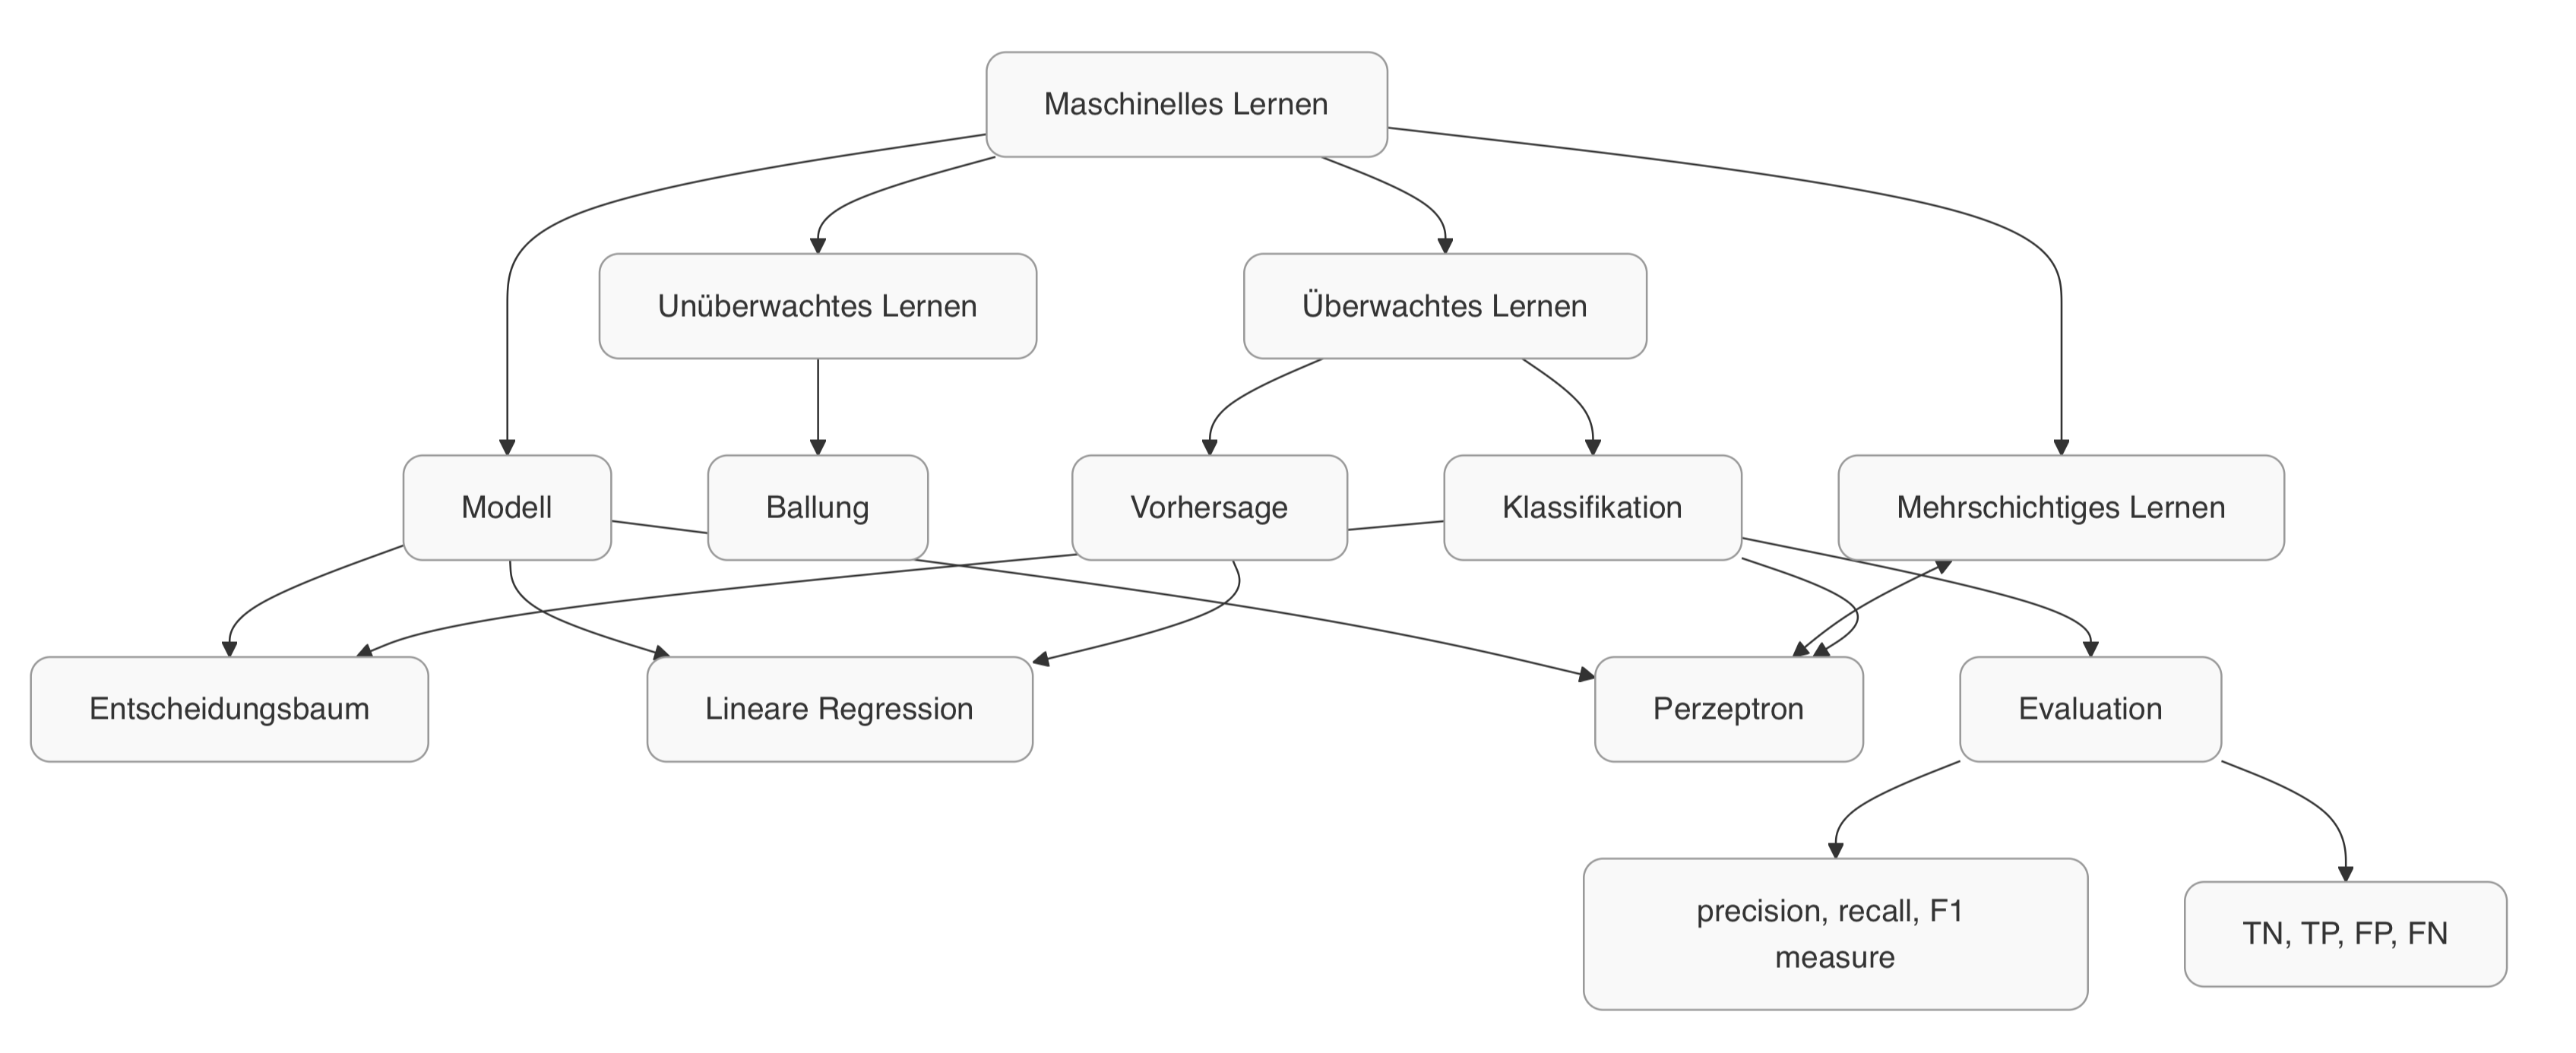
\includegraphics[width=\textwidth]{mindmap}
    \caption{Wissenswolke der wichtigsten Konzepte. }
    \label{fig:conceptmap}
\end{figure*}

Die Begriffe \textit{Mehrschichtiges Lernen}, \textit{Perzeptron} und die Evaluations-Metriken werden in dieser LPU aber nicht behandelt. Sie sind hier in der \textit{concept map} aufgeführt, um anschliessend in Kapitel \ref{sec:abschluss} aufzeigen zu können, wie der Unterricht weitergehen könnte.

\subsection{Schlussfolgerung}

Bei der Vermittlung dieses Stoffs kann also auf sehr wenig theoretisches Vorwissen zurückgegriffen werden. Allerdings erlaubt die Erfahrung der SuS mit Python, die Theorie praktisch umzusetzen, und so den Stoff zu veranschaulichen.



\section{Leitidee und Lernziele}
\label{sec:leitidee}

\subsection{Handlungsziele in der Berufsbildung}
Das Modul, auf dessen Basis die Unterrichtseinheit entstanden ist, ordnet sich in den regulären Ablauf der Ausbildung zum Applikations-Entwickler EFZ ein. Somit bestehen bereits \textit{Handlungsziele} (HZ), welche die Organisation der Arbeitswelt festgelegt hat. Diese lassen sich \href{https://www.modulbaukasten.ch/module/259/1/de-DE?title=ICT-L%C3%B6sungen-mit-Machine-Learning-entwickeln}{hier}\footnote{\url{modulbaukasten.ch/module/259/1/de-DE?title=ICT-L\%C3\%B6sungen-mit-Machine-Learning-entwickeln}} einsehen. Diese Handlungsziele werden an den Berufsschulen in \textit{Leistungsziele} (LZ) heruntergebrochen, welche durch die Verwendung bestimmter Verben (nachfolgend fettgedruckt) zum Ausdruck bringen, auf welcher Taxonomiestufe sich das LZ befindet. Die folgenden LZ habe ich also als Ersteller des Moduls aus den sehr viel allgemeiner gehaltenen, vorgegebenen HZ erstellt.

\newcounter{mainnum} % Creates a counter for the first number
\setcounter{mainnum}{1} % Set the starting number
\begin{enumerate}[label=\arabic{mainnum}.\arabic*, nosep]

    \item Ich kann für verschiedene ML-Technologien \textbf{bestimmen}, ob sie für eine gegebene Situation geeignet sind.
    \item Ich kann einer Fachperson \textbf{erkären}, warum in einer gegebenen Situation eine ML-Lösung angebracht ist.
    \item Ich kann die Kategorien des ML \textbf{angeben}.
    \item Ich kann von Hand mit Hilfe einer Erklärung für einen kleinen Datensatz gängige Modelle \textbf{berechnen}.
    \item Ich kann mithilfe einer Erklärung für einen grossen Datensatz die gängigen Modelle in python \textbf{berechnen}.

    \stepcounter{mainnum} % Increment to 2.x numbering

    \item Ich kann zu einem Thema und einer Fragestellung \textbf{bestimmen}, ob ein Datensatz dazu geeignet ist.
    \item Ich kann bei der Beschaffung eines Datensatzes die Datenschutzbestimmungen \textbf{umsetzen}.
    \item Ich kann \textbf{begründen}, warum die Datenschutzbestimmungen gelten und diese sinnvoll sind.

    \stepcounter{mainnum} % Increment to 2.x numbering

    \item Ich kann für einen gegebenen Datensatz ein Programm \textbf{entwickeln}, welches ihn für den Einsatz vorbereitet.
    \item Ich kann \textbf{bestimmen}, welche Probleme bei einem Datensatz für den Einsatz vorliegen. 
    \item Ich kann die verschiedenen Kategorien von Daten \textbf{aufzählen}.

    \stepcounter{mainnum} % Increment to 2.x numbering

    \item Ich kann einem Laien \textbf{erklären}, wie eine ML-Pipeline aufgebaut ist.
    \item Ich kann selbständig ein Programm \textbf{entwickeln}, welches meine Daten in Train- und Evaluation-Sets aufteilt.

    \stepcounter{mainnum} % Increment to 2.x numbering

    \item Ich kann für ein gegebenes Modell \textbf{bestimmen}, ob es die Anforderungen erfüllt.
    \item Ich kann \textbf{angeben}, welches die Kriterien zur Evaluation eines Modells sind.

    \stepcounter{mainnum} % Increment to 2.x numbering

    \item Ich kann mithilfe einer Anleitung auf einem Rechner eine ML-Pipeline \textbf{anwenden}.
    \item Ich kann \textbf{angeben}, wo ich Erklärungen zur Einstellung von Hyper-Parametern finde.

    \stepcounter{mainnum} % Increment to 2.x numbering

    \item Ich kann \textbf{erklären}, welche Technologien sich warum für ML-Anwendungen eignen.
    \item Ich kann \textbf{angeben}, welche gängigen Bibliotheken es für ML in Python gibt.
    
\end{enumerate}


Da die Berufsbildung den Fokus auf \textit{Handlungs-} statt \textit{Lern-Ziele} setzt, ist also eine gewisse Übersetzung nötig, welche ich im nachfolgenden Abschnitt vornehme.

\subsection{Leitidee}
In der heutigen Welt sind Daten, Algorithmen und künstliche Intelligenz allgegenwärtig – von sozialen Medien über medizinische Diagnosen bis hin zur Finanzwelt. Die Fähigkeit, algorithmisches Denken anzuwenden und grundlegende Konzepte des maschinellen Lernens zu verstehen, ist daher nicht nur für angehende Informatiker relevant, sondern für alle, die fundierte Entscheidungen in einer zunehmend digitalisierten Gesellschaft treffen müssen.

\subsubsection{Berufsschüler}

Für Berufsschüler, die eine Karriere in der IT anstreben, sind ML-Konzepte essenziell, da sie die Grundlage vieler moderner Technologien bilden. Wer als Informatiker arbeitet, wird früher oder später mit Datenanalyse, Automatisierung und KI konfrontiert. Das Verständnis von Klassifikation, Entscheidungsbäumen und Vorhersagemodellen ist daher nicht nur theoretisch interessant, sondern direkt anwendbar – sei es in der Softwareentwicklung, der Cybersicherheit oder der KI-gestützten Automatisierung.

\subsubsection{Gymnasiasten}
\label{sec:leitideegymi}

Gymnasiasten hingegen werden nicht alle Informatiker, aber sie werden in einer Welt leben und arbeiten, in der Algorithmen über Kreditzusagen, Jobempfehlungen und wissenschaftliche Erkenntnisse entscheiden. Auch in vielen wissenschaftlichen Disziplinen, insbesondere im MINT-Umfeld, spielen KI-Technologien heute bereits eine zentrale Rolle: Wer später etwa als Biologin, Chemiker oder Bauingenieurin arbeitet, wird sich intensiv mit KI-gestützten Verfahren auseinandersetzen müssen, um komplexe Projekte durchzuführen. Wer ML-Konzepte versteht, kann:

\begin{itemize}[itemsep=0.3em, parsep=0pt, topsep=1em]
   \item Kritisch mit KI-Technologien umgehen (z. B. wie funktionieren Algorithmen hinter Suchmaschinen oder Social-Media-Feeds?).
   \item Grundlegende statistische Zusammenhänge erfassen, um datenbasierte Entscheidungen zu hinterfragen.
   \item Chancen und Risiken neuer Technologien einschätzen können (z. B. Datenschutz oder Befangenheit in KI).
   \item Den Stellenwert von KI-Verfahren auch in der eigenen Fachdisziplin erkennen und reflektiert damit umgehen.
\end{itemize}

\subsubsection{Fazit}

Während Berufsschüler ML als Werkzeug für ihre berufliche Zukunft nutzen, benötigen Gymnasiasten ein fundiertes Grundverständnis, um mündige, kritische Nutzer digitaler Technologien zu sein. Die hier vermittelten Konzepte schaffen eine Brücke zwischen beiden Welten: Sie sind praxisrelevant für angehende Informatiker und gleichzeitig eine wichtige digitale Allgemeinbildung für alle anderen.


\subsection{Dispositionsziele}
\label{sec:dispziele}

Diese Dispositionsziele definieren die allgemeinen Fähigkeiten, die SuS nach der Unterrichtseinheit erwerben sollen. Die SuS sollen nicht nur ML-Algorithmen verstehen und anwenden können, sondern sich auch langfristig mit technologischen Entwicklungen auseinandersetzen können und wollen.  

\begin{enumerate}[itemsep=0.3em, parsep=0pt, topsep=0em]
    \item Nach Abschluss der Unterrichtseinheit können die SuS verschiedene Algorithmen des maschinellen Lernens unterscheiden und deren Einsatzbereiche begründen. Sie erkennen, welche Algorithmen für welche Art von Problemen geeignet sind (z. B. Klassifikation, Regression, Ballung), und entwickeln eine Intuition für die Stärken und Schwächen verschiedener ML-Ansätze. So können sie neue Algorithmen in bestehende Konzepte einordnen.

    \item Die SuS verfolgen aktuelle Entwicklungen im Bereich des maschinellen Lernens mit Interesse und reflektieren deren Auswirkungen. Sie sind motiviert, sich eigenständig über neue ML-Technologien zu informieren, etwa durch Fachartikel, Nachrichten oder wissenschaftliche Beiträge.
    Sie können neue ML-Verfahren kritisch bewerten und mit bekannten Algorithmen vergleichen, um deren Nutzen und Herausforderungen einzuschätzen.
\end{enumerate}

\subsection{Operationalisierte Lernziele}
\label{sec:oplernziele}

Zur besseren Einordnung wird zunächst die Leitidee ausdifferenziert:

\begin{enumerate}[itemsep=0.3em, parsep=0pt, topsep=0em]
  \item In einer Welt, in der immer mehr digitale Entscheidungen durch Modelle getroffen werden, ist es notwendig, dass Lernende die Funktionsweise dieser Modelle verstehen. Daher sollen die SuS die grundlegenden Kategorien maschinellen Lernens (überwacht, unüberwacht) unterscheiden und typische Anwendungsbeispiele dafür nennen können.

  \item Viele ML-Verfahren lassen sich auch ohne Informatikstudium nachvollziehen — insbesondere einfache Entscheidungsbäume oder lineare Modelle.  Aus diesem Grund sollen die SuS in der Lage sein, kleine Entscheidungsbäume und lineare Regressionsmodelle von Hand auf einem gegebenen Datensatz zu berechnen und deren Vorhersagen zu interpretieren.

  \item Damit ML-Modelle nicht als ``Black Boxes'' erscheinen, sondern als Werkzeuge verstanden werden, braucht es Erfahrungen mit konkreten Implementierungen.  Deshalb sollen die SuS eine einfache ML-Pipeline in Python mit \texttt{scikit-learn} aufbauen, ausführen und evaluieren können.

  \item Da das ML in zahlreichen wissenschaftlichen Disziplinen eine zentrale Rolle spielt, sollen die SuS zentrale Begriffe kennen, mit welchen sie können Modelle schneller verstehen, einordnen und kritisch reflektieren können.

  \item Der verantwortungsvolle Umgang mit Daten ist im Kontext des maschinellen Lernens unumgänglich. Darum sollen die SuS typische ethische Fragestellungen (Bias, Transparenz, Profiling) erkennen und reflektieren können.
\end{enumerate}

Aus diesen kleineren Leitideen ergeben sich die in Tabelle \ref{tab:lernziele} aufgeführten operationalisierten Lernziele.

\begin{table*}[ht]
\centering
\begin{tabular}{p{1.2cm}p{3.5cm}p{3.5cm}p{3.5cm}p{3.5cm}}
\hline
\textbf{Nr.} & \textbf{Endverhalten} & \textbf{Gegenstand} & \textbf{Bedingungen} & \textbf{Beurteilungs\-maßstab} \\
\hline

1 & Die SuS können die grundlegenden Kategorien des maschinellen Lernens (überwachtes und unüberwachtes Lernen) sicher unterscheiden und typische Anwendungsbeispiele nennen. 
& Kategorien des ML: überwachtes und unüberwachtes ML, Beispiele (z. B. Klassifikation, Regression, Ballung). 
& Einzelarbeit ohne Hilfsmittel, nach Einführung. 
& SuS ordnen fünf Problemstellungen korrekt zu und nennen je Kategorie ein eigenes Beispiel. \\

\hline

2 & Die SuS können kleine Entscheidungsbäume und lineare Regressionsmodelle von Hand auf einem Datensatz konstruieren und Vorhersagen berechnen. 
& Entscheidungsbaum (Klassifikation), lineare Regression (numerische Vorhersage). 
& Arbeit mit kleinen Datensätzen (Papier/Excel), Einzel- oder Partnerarbeit. 
& SuS wenden Modelle auf mindestens fünf Datenpunkte korrekt an und überprüfen mit MSE. \\

\hline

3 & Die SuS bauen in Python mit \texttt{scikit-learn} eine Pipeline (Daten laden, aufteilen, trainieren, evaluieren) und führen diese aus. 
& Standard-ML-Pipeline (z. B. Iris-Datensatz), Klassifikation oder Regression, Evaluation mit \texttt{score()} oder \texttt{classification\_report}. 
& Arbeit im Jupyter Notebook, Nutzung der Dokumentation erlaubt. 
& Pipeline läuft fehlerfrei und Evaluation wird korrekt interpretiert (z. B. Unterschied Training/Test). \\

\hline

4 & Die SuS definieren zentrale Begriffe des ML (z. B. supervised learning, model, bias, precision, recall) in eigenen Worten und wenden diese auf Beispiele an. 
& Glossararbeit mit eingeführten Fachbegriffen. 
& Einzelarbeit mit Glossar, Unterrichtsmaterialien erlaubt. 
& Die Definitionen sind allesamt korrekt und nachvollziehbar. \\

\hline

5 & Die SuS erkennen typische ethische Fragestellungen (Bias, Transparenz, Profiling) und diskutieren deren Relevanz kritisch. 
& Ethische Aspekte von ML, Datenschutzgesetz, Bias im Training, Transparenz. 
& Arbeit mit Fallbeispielen, Diskussion im Plenum. 
& Schriftliche Reflexion: SuS nennen zu jedem Aspekt ein Beispiel und mögliche Konsequenzen. \\

\hline
\end{tabular}
\caption{Operationalisierte Lernziele für diese LPU}
\label{tab:lernziele}
\end{table*}



\section{Unterrichtsplanung}
\label{sec:planung}

Die folgende Unterrichtsplanung führt die SuS systematisch vom theoretischen Fundament des maschinellen Lernens zu konkreten Implementierungen. Dabei werden sowohl kognitive als auch praktische Kompetenzen aufgebaut.

\begin{itemize}[itemsep=0.3em, parsep=0pt, topsep=0em]
  \item \textbf{Lektion 1: Zentrale Begriffe des ML}\\
  Die SuS erstellen ein eigenes Glossar mit Begriffen wie \emph{Modell}, \emph{Klassifikation}, \emph{Vorhersage}, \emph{überwachtes und unüberwachtes Lernen} etc., und formulieren erste Definitionen in eigenen Worten.

  \item \textbf{Lektion 2: Theoretische Grundlagen: Datentypen und Vorhersagen}\\
  Einführung in die Unterscheidung numerischer und kategorischer Daten, Überblick über Klassifikation, Regression und Ballung als Zieltypen maschinellen Lernens.

  \item \textbf{Lektion 3: Klassifikation mit Entscheidungsbäumen}\\
  Die SuS analysieren den Titanic-Datensatz und konstruieren von Hand einen einfachen Entscheidungsbaum zur Vorhersage des Überlebens. Ziel ist die Förderung von Intuition für Merkmalswahl und Entscheidungslogik.

  \item \textbf{Lektion 4: Regressionsmodelle}\\
  Die SuS explorieren Zusammenhänge zwischen Körpergrösse und Gewicht, formulieren einfache lineare Modelle und optimieren diese auf Basis des mittleren quadratischen Fehlers (MSE).

  \item \textbf{Lektion 5: Ballung}\\
  Vorstellung des Konzepts unüberwachten Lernens am Beispiel von \emph{k-means}; Diskussion geeigneter Anwendungsfälle (z. B. Kundensegmentierung).

  \item \textbf{Lektion 6: Statistische Grundbegriffe und Evaluation}\\
  Wiederholung der Begriffe Mittelwert, Median, Varianz sowie Einführung in Metriken wie \emph{precision}, \emph{recall} und \emph{F1-Score}; anschliessend Quiz zur Vertiefung.

  \item \textbf{Lektion 7: Ethische Dimensionen von ML}\\
  Diskussion von Bias, Transparenz und Datenschutz auf Basis konkreter Szenarien (z.B. Kreditvergabe); Reflexion zu Profiling.

  \item \textbf{Lektionen 8: Modelle mit \texttt{scikit-learn}}\\
  Die SuS setzen ML-Pipelines in \texttt{scikit-learn} um, inklusive Datenaufbereitung, \texttt{train-test-split}, Modelltraining (z. B. Entscheidungsbaum, Regression) und Evaluation.

\end{itemize}

Im nachfolgenden Kapitel wird jede Lektion als eigenes Unterkapitel aufgeführt.

\newpage
\onecolumn
\section{LPU}
\setcounter{subsection}{-1}
\subsection{IU+}
\label{sec:iuplus}

\begin{lpu}{Wer zahlt wie viel — und warum?}

\textbf{Einstiegsfrage:} Können wir Versicherungsbeiträge vorhersagen?

Wir steigen heute mit einer Frage ein, die – ganz ehrlich – auch aus einem Bewerbungsgespräch bei einer Versicherung stammen könnte: Stellen Sie sich vor, Sie arbeiten bei einer Krankenkasse. Ihnen liegen einige wenige Daten über eine Person vor: Alter, Geschlecht, Wohnort, ob sie raucht oder nicht, und deren Body-Mass-Index. \textit{Können Sie aus diesen Informationen vorhersagen, wie viel diese Person die Versicherung kosten wird?}

Die Daten, die Ihnen vorliegen, sehen wie folgt aus:

% Please add the following required packages to your document preamble:
% \usepackage[table,xcdraw]{xcolor}
% Beamer presentation requires \usepackage{colortbl} instead of \usepackage[table,xcdraw]{xcolor}
\begin{table}[h!]
\centering
\begin{tabular}{cccccc}
\rowcolor[HTML]{EFEFEF} 
{\color[HTML]{333333} age} & {\color[HTML]{333333} sex} & {\color[HTML]{333333} bmi} & {\color[HTML]{333333} smoker} & {\color[HTML]{333333} region} & {\color[HTML]{333333} health   insurance charges} \\
19                         & \female                         & 27.9                       & yes                           & southwest                     & ???                                             \\                                           
\end{tabular}
\end{table}

Was denken Sie? Wie viel könnte diese Person zahlen — eher viel oder eher weniger? Warum? Brauchen Sie weitere Informationen oder Vergleichswerte, um das entscheiden zu können?

Vermutlich schon: Sie müssen wissen, was jemand durchschnittlich an die Krankenkasse zahlt, und ob 27.9 ein hoher oder niedriger BMI ist. Sie brauchen also etwas Vorwissen, oder zumindest weitere Daten, die Ihnen als Vergleichspunkt dienen:

% Please add the following required packages to your document preamble:
% \usepackage[table,xcdraw]{xcolor}
% Beamer presentation requires \usepackage{colortbl} instead of \usepackage[table,xcdraw]{xcolor}
\begin{table}[h!]
\centering
\begin{tabular}{cccccc}
\rowcolor[HTML]{EFEFEF} 
{\color[HTML]{333333} age} & {\color[HTML]{333333} sex} & {\color[HTML]{333333} bmi} & {\color[HTML]{333333} smoker} & {\color[HTML]{333333} region} & {\color[HTML]{333333} health   insurance charges} \\
19                         & \female                         & 27.9                       & yes                           & southwest                     & ???                                             \\
18                         & \male                         & 33.77                      & no                            & southeast                     & 1725                                              \\
28                         & \male                        & 33                         & no                            & southeast                     & 4449                                              \\
33                         & \male                        & 22                         & no                            & northwest                     & 8240                                             
\end{tabular}
\end{table}

So sind Sie bereits einen Schritt weiter - Sie können einschätzen, in welchem Rahmen sich die Prämien und BMIs bewegen. Was würden Sie also raten, was diese Person zahlen könnte?

Tatsächlich zahlt diese Person eine Prämie von \textbf{16884}, was deutlich höher als die Übrigen ist; vermutlich deswegen, weil sie raucht\footnote{Dies ist ein fiktives Beispiel. In der Schweiz dürfen die Krankenkassen für die obligatorischen Grundversicherung individuelle Faktoren wie Alter, Geschlecht oder Gesundheitszustand \textit{nicht} für die Prämienberechnung verwenden. Stattdessen hängt die Höhe der Prämie vor allem vom Wohnort sowie vom gewählten Versicherungsmodell ab.}. Hätten Sie mehr vergleichbare Daten gehabt, hätten Sie dies vielleicht erahnen können.

Nun haben Sie aber nicht nur eine Person pro Tag, für die Sie eine solche Prognose machen müssen, sondern sehr viele. Sie müssen sich also auf die Hilfe eines Computers verlassen. Wir können unsere Einstiegsfrage also schärfen: \textit{Könnte ein Computer lernen, aus solchen Daten eine Prämie zu schätzen? Was müsste er dazu über viele Personen hinweg "verstehen"? Wie können wir einem Computer begreifbar machen, dass Raucher eine höhere Krankenkassenprämie zahlen?}

Wir greifen hier nun etwas vor: Dies alles ist tatsächlich möglich! Das Forschungsfeld, das sich genau mit solchen Fragen beschäftigt, wird \textbf{maschinelles Lernen} (ML) genannt.  Es gehört zur Informatik und versucht zu erklären, wie Computer aus Daten Muster erkennen und diese nutzen, um \textit{Vorhersagen} oder \textit{Entscheidungen} zu treffen, ohne dass jede einzelne Regel von Menschen programmiert werden muss. 

Maschinelles Lernen kommt heute in so vielen Bereichen zum Einsatz — von Netflix über Spotify bis zur Verkehrsplanung und Krankenversicherungen. Damit wir mit maschinellem Lernen gute Vorhersagen treffen können, brauchen Sie Daten, wie wir sie im Beispiel oben gesehen haben. Unser Einstiegsbeispiel steht als \textit{stellvertretend} für eine ganze Klasse an spannenden Problemen, für welche wir mit maschinellem Lernen Lösungen finden können.

\vspace{0.5em}
Am Ende dieser Unterrichtseinheit können Sie…

\begin{itemize}[itemsep=0.3em, parsep=0pt, topsep=0em]
  \item erklären, was maschinelles Lernen ist und wie es sich von klassischer Programmierung unterscheidet,
  \item erkennen, welche Arten von Daten es gibt und wie man sie für maschinelles Lernen vorbereitet,
  \item einfache Modelle selbst anwenden, zum Beispiel um Vorhersagen zu treffen oder Zugehörigkeit zu einer Gruppe zu erkennen,
  \item mit Python und einer speziellen Bibliothek eigene kleine ML-Projekte umsetzen,
  \item entscheiden, welcher Algorithmus für eine bestimmte Aufgabe geeignet ist,
  \item beurteilen, wie gut ein Verfahren Vorhersagen macht – und woran man das erkennt,
  \item einschätzen, welche Chancen und Risiken ML im Alltag mit sich bringt (z.B. bei Datenschutz oder Fairness).
\end{itemize}
    
\end{lpu}

\subsection{Zentrale Begriffe des ML}
\label{sec:first}
\label{sec:begriffe}
\begin{lpu}

Bevor Sie im weiteren Verlauf dieses Moduls eigene Programme zum maschinellen Lernen schreiben, ist es wichtig, dass Sie sich mit den zentralen Begriffen dieses Themas vertraut machen. Auch wenn Sie einige dieser Wörter womöglich schon gehört haben, so haben sie im Zusammenhang mit ML oft eine sehr spezifische Bedeutung.

In diesem Kapitel erarbeiten Sie sich diese Begriffe anhand eines Artikels von IBM\footnote{\href{https://www.ibm.com/think/topics/machine-learning}{\url{ibm.com/think/topics/machine-learning}}}. Der Artikel erklärt, was maschinelles Lernen ist, welche Arten es gibt und wie es in der Praxis angewendet wird.

\begin{aufgabe}{1}
Erstellen Sie ein neues, leeres Textdokument mit dem Namen \texttt{LastnameFirstname\_glossary.txt}. Das ist Ihr Glossar, welches Sie im Verlauf dieser Unterrichtseinheit mit eigenen Definitionen wichtiger Begriffe befüllen; und so in Zukunft auch eine Möglichkeit haben, sich schnell wieder in Erinnerung zu rufen, was Sie gelernt haben.

Tragen Sie darin zunächst acht Begriffe ein und formulieren Sie zu denen jeweils eine erste eigene Definition.

\newpage

\begin{itemize}[noitemsep]
  \item classification (Klassifizierung)
  \item clustering (Ballung)
  \item deep learning (mehrschichtiges Lernen)
  \item machine learning (maschinelles Lernen)
  \item model (Modell)
  \item prediction (Vorhersage)
  \item supervised learning (überwachtes Lernen)
  \item unsupervised learning (unüberwachtes Lernen)
\end{itemize}

\end{aufgabe}

Diese Aufgabe mag auf den ersten Blick etwas merkwürdig scheinen. Sie tragen eine Definition ein, obwohl Sie noch gar nicht eine klare Vorstellung davon haben können, was die Begriffe bedeuten. Das ist jedoch eine wertvolle \textit{Lernstrategie}: So halten Sie sich einerseits vor Augen, nach welchen Informationen Sie genau in dem Artikel suchen. Damit wird die Lektüre zielgerichteter und hilft insbesondere SuS, welche zu konzentrieren über längere Zeit Mühe haben. Andererseits machen Sie explizit, was an vagen Ideen in Ihrem Kopf schon vorhanden ist: Vielleicht haben Sie bereits eine Intuition oder ein Halbwissen, was ein Begriff bedeuten könnte. So können Sie diese bewusst vergleichen mit der Definition, die im Text angeboten wird.

Darum machen Sie erste Definitionen noch \textit{bevor} Sie den Artikel lesen. Nach der Lektüre können Sie Ihre Definitionen anpassen.

\begin{aufgabe}{2}
Lesen Sie nun den Artikel "Was ist maschinelles Lernen" aufmerksam durch. 
\end{aufgabe}

\textbf{Hinweis:} Der Artikel ist anspruchsvoll. Lassen Sie sich nicht entmutigen, wenn Sie nicht alles auf Anhieb verstehen.

\begin{artikelbox}

\artikelheader{Maschinelles Lernen (ML)}
\textit{Ursprünglich auf Englisch unter \href{https://www.ibm.com/cloud/learn/machine-learning}{\url{ibm.com/cloud/learn/machine-learning}}, am 1.1.2022 ins Deutsche übersetzt durch \url{nicola.colic@bbbaden.ch}.}

Diese Einführung ins maschinelle Lernen gibt eine Übersicht über dessen Geschichte, wichtige Definitionen, Anwendungen und Probleme innerhalb der heutigen Geschäftswelt.

\artikelsubheader{Was ist ML?}
ML ist ein Zweig der künstlichen Intelligenz und der Computerwissenschaften, welcher auf der Verwendung von Daten und Algorithmen fokussiert, um die Art wie Menschen lernen zu imitieren und schrittweise seine Genauigkeit verbessert.
IBM hat eine lange Geschichte mit ML. Von einem Mitarbeiter, Arthur Samuel, wird gesagt, er habe den Begriff "machine learning" mit seiner Forschung über ein Schachspiel geprägt. Robert Nealey, selbsternannter Schachmeister, spielte 1962 das Spiel auf einem IBM 7094-Computer und verlor gegen den Computer. Verglichen mit was heute möglich ist scheint dieser Erfolg beinahe trivial, aber er wird als einer der bedeutendsten Meilensteine im Feld der künstlichen Intelligenz betrachtet. In den kommenden Jahrzehnten ermöglichten die technologischen Weiterentwicklungen bezüglich Speicherplatzes und Rechenleistung einige innovative Produkte, die wir heute kennen und lieben, so wie beispielsweise der Vorschlags-Algorithmus von Netflix oder selbststeuernde Autos.
ML ist ein wichtiger Teil des wachsenden Feldes der Datenwissenschaft. Durch statistische Methoden werden Algorithmen trainiert, um Klassifikationen oder Vorhersagen zu treffen, und dabei Schlüsselerkenntnisse innerhalb von Datenschürf-Projekten zu gewinnen. Diese Erkenntnisse liegen Entscheidungen innerhalb Applikationen und der Geschäftswelt zugrunde, wobei sie idealerweise einen Einfluss auf Messgrössen bezüglich des Wachstums haben. Während "big data" wächst, wächst auch die Nachfrage des Marktes für Datenwissenschaftler, welche bei der Erkennung der wichtigsten Geschäftsfragen Unterstützung leisten müssen und die Daten, die jene beantworten, finden.

\artikelsubheader{ML vs. mehrschichtiges Lernen vs. neurale Netzwerke}
Weil mehrschichtiges Lernen und ML austauschbar verwendet werden, lohnt es sich die Nuancen der beiden zu verstehen. ML, mehrschichtiges Lernen und neurale Netzwerke sind alle Unterfelder der künstlichen Intelligenz. Allerdings ist mehrschichtiges Lernen ein Unterfeld von ML, und neurale Netzwerke wiederum ein Unterfeld von mehrschichtigem Lernen.
Mehrschichtiges Lernen und ML unterscheiden sich darin, wie die jeweiligen Algorithmen lernen. Mehrschichtiges Lernen automatisiert vieles der Auswahl von geeigneten Merkmalen, und eliminiert damit einen Teil der menschlichen Mitarbeit, die anderenfalls notwendig ist, und somit grössere Datensätze verwertbar macht. Man kann sich mehrschichtiges Lernen als skalierbares ML vorstellen (wie Lex Fridman in einer MIT-Vorlesung gesagt hat). Klassisches, nicht-mehrschichtiges ML hängt mehr von menschlichen Eingriffen ab. Menschliche Experten suchen sich bestimmte Merkmale aus, auf welche der Algorithmus achten soll, und so braucht diese Art oft besser strukturierte Daten, um zu lernen.
Mehrschichtiges Lernen kann einen Nutzen aus annotierten Datensätzen ziehen, was auch überwachtes Lernen genannt wird, um seine Algorithmen auszuwählen; aber es braucht nicht unbedingt einen annotierten Datensatz. Es kann unstrukturierte Daten in Rohform (beispielsweise Text oder Bilder) verarbeiten, und kann automatisch bestimmen, welche Merkmale dieser Daten die unterschiedlichen Kategorien der Daten voneinander unterscheiden. Im Gegensatz zu ML braucht es dazu keine menschlichen Eingriffe, was uns ermöglicht, ML auf interessante Weise zu skalieren. Mehrschichtiges Lernen und neuronale Netzwerke sind der Grund, warum es zu Fortschritt in den Feldern der maschinellen Verarbeitung natürlicher Sprache, Spracherkennung und maschinellen Sehens gekommen ist.
Neurale Netzwerke, oder artifizielle, d.h. künstliche, neurale Netzwerke, bestehen aus Schichten von Knoten, wovon eine die Eingabeschicht, eine oder mehrere versteckte Schichten, und eine die Ausgabeschicht ist. Jeder Knoten, oder artifizielles Neuron, ist mit einem anderen verbunden und hat ein zugeordnetes Gewicht und einen Grenzwert. Wenn die Ausgabe irgendeines einzelnen Knotens über diesem Grenzwert liegt, dann ist der Knoten aktiviert und schickt Daten zur nächsten Schicht des Netzes. Ansonsten werden keine Daten zur nächsten Schicht gesendet. Das "mehrschichtig" im mehrschichtigen Lernen bezeichnet den Umstand, dass es mehr als eine Schicht in einem neuralen Netz gibt. Ein neurales Netz, welches aus mehr als drei Schichten besteht (wobei Eingabe- und Ausgabeschicht mitzählen), gilt als mehrschichtiger Lern-Algorithmus oder als ein mehrschichtiges neurales Netz. Ein neurales Netz, welches lediglich zwei oder drei Schichten hat, ist einfach ein neurales Netz.

\newpage

\artikelsubheader{Wie ML funktioniert}
UC Berkeley teilt das Lernen eines ML-Algorithmus' in drei Teile ein:
\begin{enumerate}
\item Entscheidungsprozess: Für gewöhnlich werden ML-Algorithmen benutzt, um Klassifikationen oder Vorhersagen zu treffen. Ausgehend von einigen Eingabe-Daten, welche annotiert oder nicht sein können, produziert der Algorithmus eine Schätzung bezüglich eines Musters in den Daten.
\item Eine Fehlerfunktion, welche die Vorhersage des Modells evaluiert. Wenn es Beispiele gibt, dann kann die Fehlerfunktion einen Vergleich anstellen, um die Genauigkeit des Modells zu bestimmen.
\item Ein Modell-Optimierungsprozess: Wenn das Modell sich besser an die Datenpunkte im Lern-Datensatz anpasst, dann werden die Gewichte angepasst um den Unterschied zwischen dem Beispiel und der Schätzung des Modells. Der Algorithmus wiederholt diesen Evaluations- und Optimierungsprozess, und aktualisiert so die Gewichte selbständig, bis ein bestimmter Grenzwert an Genauigkeit erreicht wurde.
\end{enumerate}

\artikelsubheader{ML-Methoden}
ML-Klassifikatoren lassen sich in drei Hauptkategorien einteilen:

\textbf{Überwachtes ML}
Überwachtes Lernen oder überwachtes ML ist definiert dadurch, dass es annotierte Datensätze gebraucht, um Algorithmen zu trainieren, welche Daten klassifizieren oder Resultate korrekt vorhersagen. Eingabedaten werden in das Modell gespiesen, dieses passt seine Werte an, bis das Model ausreichend passend ist. Dies passiert als Teil eines Kreuzvalidierungs-Prozesses um sicherzustellen, dass dem Modell keine Über- oder Unteranpassung unterläuft. Überwachtes lernen hilft Organisationen, eine Vielzahl echter Probleme grosser Ordnung zu lösen, wie etwa das Klassifizieren von unerwünschten E-Mails in einem separaten Ordner des Posteingangs. Zu den Methoden, welche beim überwachten Lernen gebraucht werden, gehören neurale Netze, naive Bayes-Klassifikatoren, lineare und logistische Regressionen, random forest, Stützvektormaschinen und weitere.


\textbf{Unüberwachtes Lernen oder unüberwachtes ML}
Dies benutzt ML-Algorithmen, um unannotierte Datensätze zu analysieren und zu ballen. Diese Algorithmen erkennen versteckte Muster oder Datengruppen, ohne dass Menschen eingreifen müssen. Ihre Fähigkeit, Ähnlichkeiten und Unterschiede in Informationen zu finden, machen sie zu einer idealen Lösung für explorative Daten-Analyse, Querverkaufsstrategien, Kunden-Segmentierung, Bilder- und Mustererkennung. Sie wird auch gebraucht, um die Anzahl Merkmale eines Modells durch Dimensionalitätsreduktion zu verkleinern; Hauptkomponentenanalyse und Singulärwertanalyse sind zwei Ansätze hierzu. Andere Algorithmen, welche in unüberwachtem Lernen gebraucht warden, sind neurale Netze, der k-means-Algorithmus, probabilistische Ballungsmethoden und weitere.

\textbf{Halbüberwachtes Lernen}
Dies stellt die goldene Mitte zwischen überwachten und unüberwachtem Lernen dar. Während des Trainings benutzt es einen kleineren annotierten Datensatz, um die Klassifikation und Erkennung von Merkmalen eines grösseren, unannotierten Datensatzes voranzutreiben. Halbüberwachtes Lernen kann damit das Problem lösen, nicht genug annotierte Daten zu haben (oder es sich nicht leisten zu können, so viele Daten zu annotieren), um einen überwachten Lernalgorithmus zu trainieren.

\textbf{Bestärkendes ML}
Ein verhaltensgesteuertes ML-Modell, das ähnlich zum überwachten Lernen ist, aber bei dem der Algorithmus nicht mit Beispieldaten trainiert wird. Dieses Modell lernt fortlaufend durch Versuch und Irrtum. Eine Reihe von erfolgreichen Ergebnissen wird verstärkt, um die beste Empfehlung oder Handlungsdevise für ein gegebenes Problem zu entwickeln.
Das IBM Watson-System, welches 2011 Jeopardy! gewonnen hat, ist ein gutes Beispiel. Das System benutzt bestärkendes Lernen, um zu entscheiden, ob es sich an einer Frage versuchen soll, welches Quadrat es auf dem Spielbrett aussuchen soll und wie hoch sein Einsatz sein soll.

\artikelsubheader{Praktische ML-Anwendungsfälle}
Es folgen einige Beispiele von ML, welche im täglichen Leben vorkommen: 
\begin{itemize}
\item (Automatische) Spracherkennung, wird auch computergesteuerte Spracherkennung oder Textsynthese genannt, was die Umwandlung von menschlicher Sprache in geschriebenes Wort mithilfe von maschineller Sprachverarbeitung bedeutet. Viele Mobilgeräte verfügen über Spracherkennung, um sprachgesteuerte Suchen auszuführen, wie etwa Sir, oder es leichter zu machen, Textnachrichten zu verfassen.
\item Kundendienst: Textbasierte Dialogsysteme verdrängen Menschen in der customer journey. Sie beantworten Oft Gestellte Fragen zu Themen wie Fracht oder bieten personalisierte Beratung an, betreiben Querverkäufe oder empfehlen Grössen für Benutzer. Sie ändern somit die Art, wie wir über Kundenbindung auf Netzseiten und sozialen Medien nachdenken. Beispiele sind virtuelle Agenten im elektronischen Handel, Nachrichten-Applikationen wie Slack und Facebook Messenger, und die Aufgaben, die virtuelle Assistenten und Sprachassistenten übernehmen.
\item Maschinelles Sehen: Diese Technologie der künstlichen Intelligenz ermöglicht es Computern und System, sinnvolle Informationen aus digitalen Bildern, Filmen und anderen visuellen Eingaben zu extrahieren, und Handlung basierend auf diesen Eingaben zu ergreifen. Diese Fähigkeit, Empfehlungen auszusprechen, unterscheidet sie von Bilderkennungs-Aufgaben. Basierend auf faltenden neuronalen Netzen hat das maschinelle Sehen Anwendungen im Annotieren von Bildern in den sozialen Medien, Analyse von Röntgenbildern im Gesundheitsbereich oder selbststeuernde Autos im Automobil-Sektor.
\item Empfehlungs-Systeme: Algorithmen der künstlichen Intelligenz helfen basierend auf vergangenen Daten über vergangenes Kaufverhalten dabei, Tendenzen zu entdecken, welche benutzt werden können, um effektivere Querverkaufsstrategien zu entwickeln. Dies wird benutzt, um relevante Empfehlungen für weitere Käufe während des Kaufs den Kunden anzuzeigen.
\item Automatisierter Aktienhandel: Entwickelt, um Aktien-Portfolios zu optimieren, generieren Plattformen des Hochfrequenzhandels abertausende Transaktionen jeden Tag ohne menschliche Eingriffe.
\end{itemize}
\end{artikelbox}

\begin{hinweis}
    Der Artikel von IBM wurde selbst mithilfe maschinellen Lernens ins Deutsche übertragen. Eine wichtige Anwendung von ML ist nämlich die \textit{maschinelle Übersetzung}. Während diese Unterrichtseinheit nicht ganz so weit geht, so haben Sie am Ende davon die Möglichkeit, sich in der natürlichen Sprachverarbeitung etwas zu vertiefen. Diese stellt die Grundlage für die maschinelle Übersetzung dar! 
    
    Einige Formulierungen sind darum sprachlich nicht perfekt, inhaltlich aber korrekt. Wenn Sie sich unsicher sind, lesen Sie die englische Originalfassung.
\end{hinweis}
\end{lpu}

\subsection*{Didaktische Überlegungen}
Die Einführung zentraler Begriffe des maschinellen Lernens anhand eines Artikels verfolgt ein bewusst gewähltes didaktisches Ziel: Anders als viele klassische Informatikthemen unterliegt das Feld des maschinellen Lernens einem rasanten Wandel — sowohl inhaltlich als auch in der verwendeten Terminologie. Begriffe, Konzepte und Methoden ändern sich schnell, und neue Verfahren treten regelmässig hinzu. Für Sie als zukünftige Informatikerinnen und Informatiker bedeutet das, dass nicht allein das Verstehen von heute gängigen Definitionen zählt, sondern vor allem die Fähigkeit, sich selbständig in neue Inhalte einzuarbeiten.

Die Arbeit mit einem authentischen übersetzten Fachartikel fördert diese Kompetenz gezielt: Sie üben, wie man aus einem anspruchsvollen Text zentrale Informationen filtert, eigene Definitionen entwickelt und die Bedeutung neuer Begriffe im Kontext versteht. Diese Fähigkeit zur eigenständigen Wissensaneignung ist nicht nur im Bereich ML zentral, sondern eine Schlüsselkompetenz in der gesamten Informatik und Technik.

Zudem stärkt die Auseinandersetzung mit einem englischsprachigen Originaltext (optional) Ihre Fachsprachkompetenz – ein weiterer Aspekt, der gerade im internationalen Arbeitsumfeld der Informatik von wachsender Bedeutung ist.

\subsection*{Musterlösung}

\begin{itemize}
  \item \textbf{classification (Klassifizierung):} Ein ML-Verfahren, bei dem ein Algorithmus entscheidet, zu welcher vorgegebenen Kategorie ein Datensatz gehört.
  \item \textbf{clustering (Ballung):} Eine Methode des unüberwachten Lernens, bei der ähnliche Datenpunkte automatisch zu Gruppen zusammengefasst werden.
  \item \textbf{deep learning (mehrschichtiges Lernen):} Eine spezielle Form des maschinellen Lernens, die mit vielen Schichten künstlicher neuronaler Netze arbeitet.
  \item \textbf{machine learning (maschinelles Lernen):} Ein Teilbereich der KI, bei dem Systeme aus Beispielen lernen, um Aufgaben zu lösen, ohne explizit programmiert zu sein.
  \item \textbf{model (Modell):} Das Ergebnis eines Lernprozesses, das genutzt wird, um Vorhersagen oder Klassifikationen basierend auf neuen Daten zu treffen.
  \item \textbf{prediction (Vorhersage):} Die Fähigkeit eines Modells, ein Ergebnis für neue, unbekannte Datenpunkte zu schätzen.
  \item \textbf{supervised learning (überwachtes Lernen):} Eine Methode, bei der ein Modell mit Daten trainiert wird, deren richtige Ergebnisse bereits bekannt sind.
  \item \textbf{unsupervised learning (unüberwachtes Lernen):} Eine Methode, bei der das Modell Muster in Daten erkennt, ohne dass vorab richtige Ergebnisse bekannt sind.
\end{itemize}

\subsection{Datentypen und Vorhersagen}
\begin{lpu}

Maschinelles Lernen lebt von den Daten – ohne Daten keine Erkenntnis. Damit Sie sinnvolle Modelle entwickeln k\"onnen, m\"ussen Sie Ihre Daten kennen, analysieren und korrekt aufbereiten. Das beginnt damit, die unterschiedlichen Datentypen zu verstehen, die im maschinellen Lernen auftreten. Nur so k\"onnen Sie entscheiden, welcher Algorithmus sich f\"ur Ihre Aufgabenstellung eignet.

\begin{aufgabe}{1}
Betrachten Sie die folgende Tabelle mit Informationen zu fiktiven Personen: \vspace{0.5em}

\begin{center}
\begin{tabular}{|l|l|l|l|l|}
\hline
\textbf{Name} & \textbf{Alter} & \textbf{Geschlecht} & \textbf{Gewicht (in kg)} & \textbf{Region} \\
\hline
Anna   & 22    & weiblich  & 55   & Nordwest \\
Luca   & 35    & m\"annlich & 82   & S\"udost \\
Fatima & 41    & weiblich  & 63  & Zentrum \\
\hline
\end{tabular}
\end{center}

Sehen Sie Unterschiede in der Art dieser Daten? Versuchen Sie in Worte zu fassen, worin sich die einzelnen Spalten unterscheiden.

\textbf{Hinweis:} Stellen Sie sich die Frage: \textit{Welche dieser Angaben kann ich sinnvoll miteinander verrechnen, zum Beispiel, um den Durchschnitt zu bestimmen?}
\end{aufgabe}

Es gibt ganz unterschiedliche Arten, Daten einzuordnen und zu analysieren. Doch für diese Unterrichtseinheit ist die nachfolgende Unterscheidung zielführend, weil sie uns später erlaubt, die richtigen Methoden auszusuchen.

\begin{theorie}
Im maschinellen Lernen unterscheidet man zwei Arten von Daten:
\begin{itemize}
  \item \textbf{numerische Daten} (\emph{numerical data}): messbare Werte wie Alter, Temperatur oder Einkommen. Diese kann man verrechnen.
  \item \textbf{kategorische Daten} (\emph{categorical data}): beschreibende Werte wie Farbe, Geschlecht oder Region. Diese kann man nicht sinnvoll verrechnen.
\end{itemize}
\end{theorie}

\begin{aufgabe}{2}
Ordnen Sie folgende Merkmale einer Person den zwei Datentypen zu: \emph{Alter, Geschlecht, Nationalit\"at, Gewicht, Wohnregion, Schulabschluss}. Begr\"unden Sie Ihre Entscheidungen.
\end{aufgabe}

Im Beispiel oben ist die Zuordnung weitgehend eindeutig: Man kann sich zwar überlegen, ob man bei Schulabschluss eine Note ausgibt oder auflistet, ob jemand eine EFZ, eine Matur oder einen anderen Abschluss gemacht hat. Im ersten Fall hätten wir es dann mit \textit{numerischen} Daten zu tun, und im zweiten Fall mit \textit{kategorischen}. Doch aufgepasst! Was, wenn wir alle möglichen Abschlüsse auflisten, und nur die \textbf{Nr.} verwenden, um anzugeben, welchen Abschluss jemand erreicht hat?

\begin{table}
\begin{center}
\begin{tabular}{|c|l|}
\hline
\textbf{Nr.} & \textbf{Abschluss} \\
\hline
1 & obligatorische Schule abgeschlossen \\
2 & Berufslehre mit EFZ \\
3 & Berufsmaturität \\
4 & Fachmittelschule (FMS) \\
5 & Gymnasiale Maturität \\
6 & Höhere Fachschule (HF) \\
7 & Fachhochschule (FH) Bachelor \\
8 & Universität / ETH Bachelor \\
9 & Fachhochschule (FH) Master \\
10 & Universität / ETH Master \\
11 & Doktorat (Dr./PhD) \\
\hline
\end{tabular}
\caption{Typische schulische und tertiäre Abschlüsse in der Schweiz, nummeriert.}
\label{tab:abschluesse}
\end{center}
\end{table}

Aufgepasst also vor \textbf{falschen Freunden}! In diesem Fall sind 5, 7 und 8 (zum Beispiel) zwar Zahlen, aber stellen trotzdem \textit{kategorische} Daten dar. Wir können zwar theoretisch diese Zahlen verrechnen, doch bedeuten die numerischen Werte nichts. Welchem Abschluss würde eine 3.5 entsprechen?

\begin{theorie}
Viele Algorithmen im ML k\"onnen nur mit Zahlen arbeiten. Deshalb m\"ussen kategorische Daten oft in Zahlen umgewandelt werden. Die Daten bleiben kategorisch, wobei jeder Kategorie eine Zahl zugeordnet wird.
\end{theorie}

Auch numerische Daten m\"ussen oft vorbereitet werden: Manche ML-Algorithmen reagieren empfindlich darauf, wenn sich numerische Werte nicht zwischen $[0,1]$ bewegen. Das nachfolgende Beispiel veranschaulicht dies:

\begin{aufgabe}{3}
Sie haben einen Datensatz (Person X) mit den Werten: \texttt{Alter = 28}, \texttt{Einkommen = 78000 CHF}. Welche der folgenden Personen ist \textit{ähnlicher}? Begründen Sie Ihre Wahl:
\begin{itemize}
  \item Person A: Alter = 26, Einkommen = 50\,000
  \item Person B: Alter = 40, Einkommen = 79\,000
\end{itemize}
Wie würden Sie argumentieren, wenn Sie erfahren würden, dass die \textit{andere} Person, als die, für die Sie sich ursprünglich entschieden haben, ähnlicher wäre?
\end{aufgabe}

Die Intuitionen können hier auseinander gehen, und für einen Computer reichen solche sowieso nicht aus: Wir müssen den \textit{Abstand} von X zu A und zu B mathematisch sauber definieren, damit wir die Frage beantworten können.

Ein naiver Ansatz wäre, diesen Abstand zwischen den Personen so zu berechnen, dass wir also die Differenz in den einzelnen Merkmalen aufsummieren.

\textbf{Abstand zu Person A:} $|28 - 26| + |78\,000 - 50\,000| = 2 + 28\,000 = 28\,002$ \\
\textbf{Abstand zu Person B:} $|28 - 40| + |78\,000 - 79\,000| = 12 + 1000 = 1012$

Dieser Vergleich zeigt ein Problem: Das Einkommen überwiegt aufgrund seines viel grösseren Zahlenbereichs deutlich. In dieser Rechenart müsste Person B 27\,003 Jahre alt sein, bevor sie X ähnlicher als A wäre. Völlig sinnlos, denn wer ein solches Alter erreicht, hat ungeachtet der Einkommensverhältnisse mit niemandem überhaupt eine Ähnlichkeit!

Unser Algorithmus „sieht“ also fast nur den Unterschied im Einkommen; einfach deshalb, weil sich das Einkommen in viel grösseren Dimensionen bewegt als das Alter. In der Schweiz bewegt sich der Lohn für 80\% der Einwohner zwischen 36\,000 und 120\,000 Franken; die älteste Schweizerin ist fast 113 Jahre alt geworden.

Genau hier kommt das sogenannte \emph{Skalieren} ins Spiel. Um  Merkmale vergleichbar zu machen, die auf unterschiedlichen Grössenordnungen gemessen werden, werden sie auf denselben Wertebereich gebracht – meistens auf ein Intervall zwischen 0 und 1. 

\begin{theorie}
    Um einen Wertebereich zu skalieren, geht man wie folgt vor: Man bestimmt für jedes Merkmal den kleinsten und grössten Wert im Datensatz, und rechnet dann:
    \[
\text{Skalierter Wert} = \frac{\text{aktueller Wert} - \text{Minimum}}{\text{Maximum} - \text{Minimum}}
\]
\end{theorie}

\textbf{Skalierung visuell erklärt:}

\begin{center}
\begin{tikzpicture}
  % Achse Einkommen (original)
  \draw[->] (0,0) -- (6.5,0) node[right] {\small Einkommen [CHF]};
  \foreach \x/\v in {0/50'000, 3/64'500, 6/79'000} {
    \draw (\x,0.1) -- (\x,-0.1) node[below] {\small \v};
  }
  \draw[fill=black] (5.79,0) circle (2pt) node[above] {\scriptsize 78'000};

  % Achse Einkommen (skaliert)
  \draw[->] (0,-2) -- (6.5,-2) node[right] {\small Einkommen (skaliert)};
  \foreach \x/\v in {0/0, 3/0.5, 6/1} {
    \draw (\x,-1.9) -- (\x,-2.1) node[below] {\small \v};
  }
  \draw[fill=black] (5.79,-2) circle (2pt) node[above] {\scriptsize $\approx 0.97$};
\end{tikzpicture}
\end{center}



Wie die Abbildung zeigt, wird ein Wert wie 78\,000 CHF durch die Skalierung auf ca. 0.97 gebracht – bezogen auf ein Gesamtintervall zwischen 50\,000 und 79\,000 CHF, also dem Minimum und dem Maximum in unseren vorliegenden Daten. Alle anderen Werte im Datensatz werden entsprechend transformiert. So werden Unterschiede zwischen Alters- und Einkommensdaten rechnerisch vergleichbar, auch wenn sie ursprünglich in ganz unterschiedlichen Grössenordnungen vorliegen.

Wenden wir dies auf unser Beispiel an. Das kleinste Alter ist 28, das grösste 40. Daraus ergibt sich:

\begin{itemize}
  \item Person X: $\frac{28 - 20}{40} = 0.20$
  \item Person A: $\frac{26 - 20}{40} = 0.15$
  \item Person B: $\frac{40 - 20}{40} = 0.50$
\end{itemize}

\begin{aufgabe}{4}
    Berechnen Sie auf dieselbe Art nun die skalierten Einkommen für X, A und B. Daraufhin können Sie durch Aufsummieren der Unterschiede den Abstand von X zu A und zu B berechnen, und mathematisch sauber sagen, wem X mehr ähnelt.
\end{aufgabe}

Dieser einfache Schritt – das Skalieren – ist zentral für viele Algorithmen des maschinellen Lernens. Ohne ihn kann es passieren, dass ein einzelnes Merkmal alle anderen dominiert, nur weil es in grösseren Zahlen ausgedrückt ist. Das hat nichts mit seiner inhaltlichen Wichtigkeit zu tun, sondern ist schlicht ein Nebeneffekt der unterschiedlichen Grössenordnungen (oder auch \textit{Skalen}) genannt.

\begin{aufgabe}{5}
\textbf{Welche Schülerin ist Ihnen am ähnlichsten?}

Vier Schülerinnen einer Klasse haben folgende Angaben zu ihrer durchschnittlichen Bildschirmzeit unter der Woche (in Minuten) und ihrer Schlafdauer pro Nacht (in Stunden) gemacht:

\begin{center}
\begin{tabular}{|l|c|c|}
\hline
\textbf{Name} & \textbf{Bildschirmzeit} (in Minuten) & \textbf{Schlafdauer} (in Stunden) \\
\hline
Sophie & 180 & 7.5 \\
Elena  & 240 & 6.0 \\
Mia    & 120 & 8.0 \\
Nora   & 300 & 6.5 \\
\hline
\end{tabular}
\end{center}

Was sind Ihre eigenen Werte? 

\begin{enumerate}
  \item Skalieren Sie alle Werte (auch die Ihrigen) auf einen Bereich von 0 bis 1.
  \item Berechnen Sie für jede der vier Schülerinnen den Abstand zu Ihren eigenen Werten.
  \item Wer ist Ihnen rechnerisch am ähnlichsten? Entspricht das auch Ihrem Gefühl?
\end{enumerate}

\end{aufgabe}

Viele ML-Bibliotheken übernehmen das Skalieren automatisch für Sie. Dennoch ist es wichtig, zu verstehen, warum das gemacht wird – und wann es sinnvoll ist. Gerade bei Algorithmen wie KNN (k-nearest neighbours), den Sie später noch kennenlernen werden, oder bei neuronalen Netzen ist das korrekte Skalieren der Eingabedaten entscheidend!

\begin{theorie}
\textbf{Normalisierung (Skalierung auf [0, 1])}

Wenn ein Merkmal \( x \) im Datensatz einen Minimalwert \( x_{\text{min}} \) und einen Maximalwert \( x_{\text{max}} \) hat, kann man jeden Wert \( x_i \) wie folgt auf den Bereich zwischen 0 und 1 skalieren:

\[
x_i^{\text{skaliert}} = \frac{x_i - x_{\text{min}}}{x_{\text{max}} - x_{\text{min}}}
\]

Dies stellt sicher, dass alle Merkmale vergleichbare Wertebereiche haben – unabhängig davon, ob sie ursprünglich in Franken, Jahren oder Prozentpunkten angegeben wurden.
\end{theorie}

Es gibt auch andere Verfahren zur Skalierung, aber diese Unterrichtseinheit beschränkt sich auf die Skalierung auf $[0,1]$.

Nun, da wir wichtige Grundlagen zu den Daten gelegt haben, müssen wir noch einige Begriffe schärfen, bevor wir mit den ersten Algorithmen loslegen können. Wie Sie in Kapitel \ref{sec:begriffe} gesehen haben, ist der generelle Ablauf im maschinellen Lernen folgender:

\begin{figure}
\begin{center}
\begin{tikzpicture}[
  node distance=1.8cm and 1.2cm,
  every node/.style={font=\sffamily},
  process/.style={draw, thick, rectangle, rounded corners, minimum width=2.8cm, minimum height=1cm, align=center, fill=blue!5},
  data/.style={draw, thick, rectangle, minimum width=2.8cm, minimum height=1cm, align=center, fill=gray!10},
  arrow/.style={->, thick}
]

% Nodes
\node[data] (data) {Trainingsdaten};
\node[process, right=of data] (training) {Training};
\node[data, right=of training] (model) {gelerntes Modell};
\node[data, below=of model] (newdata) {neue Daten};
\node[process, left=of newdata] (predict) {Vorhersage};
\node[data, left=of predict] (output) {Ergebnis};

% Arrows
\draw[arrow] (data) -- (training);
\draw[arrow] (training) -- (model);
\draw[arrow] (newdata) -- (predict);
\draw[arrow] (model) -- (predict);
\draw[arrow] (predict) -- (output);

\end{tikzpicture}
\end{center}
\caption{Der allgemeine Ablauf beim maschinellen Lernen.}
\end{figure}


\begin{theorie}
\textbf{Vorhersagen} (englisch: \emph{predictions}) sind zentrale Aufgaben im maschinellen Lernen. Ein Modell lernt aus vorhandenen Daten, um f\"ur neue Datenpunkte eine Sch\"atzung abzugeben.

Unterschieden werden:
\begin{itemize}
  \item \textbf{numerische Vorhersagen} – z.\,B. Temperatur, Preis, Gewicht (dafür werden wir später die \emph{Regression} verwenden)
  \item \textbf{kategorische Vorhersagen} – z.\,B. Wetterart, Geschlecht, Produktkategorie (das nennen wir \emph{Klassifikation})
\end{itemize}
\end{theorie}

\begin{aufgabe}{6}
\textbf{Welche Art von Vorhersage liegt vor?} Entscheiden Sie f\"ur jede der folgenden Fragestellungen, ob eine numerische oder eine kategorische Vorhersage gefragt ist:
\begin{itemize}
  \item Wie hoch wird der Umsatz im n\"achsten Quartal sein?
  \item Ist eine E-Mail Spam oder nicht?
  \item Welche Temperatur herrscht morgen in Ihrer Stadt?
  \item Welche Kategorie passt zu einem Kleidungsst\"uck im Online-Shop?
\end{itemize}
\end{aufgabe}

\begin{hinweis}
Manche Aufgabenstellungen enthalten beides: numerische und kategorische Aspekte. Solche \glqq zusammengesetzten\grqq{} Daten werden im fortgeschrittenen ML ebenfalls behandelt.
\end{hinweis}

Unstrukturierte Daten – wie Bilder, Sprache oder Texte – lassen sich schwerer vorhersagen. Hierzu braucht es spezielle Algorithmen, z.\,B. tiefe neuronale Netze. Diese Themen sprengen den Rahmen dieses Moduls, geh\"oren aber zu den spannendsten aktuellen Entwicklungen.
\end{lpu}

\subsection*{Musterlösung}

\begin{aufgabe}{1}
Die Tabelle enthält verschiedene Arten von Daten, die sich auf unterschiedliche Weise analysieren und verarbeiten lassen. Eine zentrale Unterscheidung besteht darin, ob die Daten \emph{numerisch} oder \emph{kategorisch} sind. Dabei helfen folgende Überlegungen:

\begin{itemize}
    \item \textbf{Name:} Diese Spalte enthält Zeichenketten (\textit{strings}). Sie dienen einzig der Identifikation der Personen. Eine mathematische Operation (wie Addition oder Durchschnitt) ist sinnlos; aber man könnte sie sortieren (zum Beispiel alphabetisch). Aber hätte man deutlich mehr Einträge, dann wäre eine statistische Auswertung möglich, zum Beispiel eine Analyse nach Häufigkeit von Namen.
    
    \item \textbf{Alter:} Das Alter ist eine \emph{numerische} (in diesem Fall: metrische) Grösse, mit der sich sinnvolle Rechenoperationen durchführen lassen. Man kann z.\,B. das durchschnittliche Alter berechnen, Altersverteilungen analysieren oder Schwellenwerte (z.\,B. „über 30“) verwenden. Man könnte auch Altersgruppen bilden (z.\,B. „jung“, „mittelalt“, „alt“), was das Alter in ein \emph{ordinales Merkmal} verwandeln würde. Diese Umcodierung ist in ML-Anwendungen üblich.

    \item \textbf{Geschlecht:} Hier handelt es sich um \emph{kategorische} Daten mit verschiedenen Möglichkeiten („männlich“ und „weiblich“, aber vielleicht auch "non-binär" oder "divers"). Eine numerische Verrechnung ist nicht sinnvoll. Eine  Umcodierung (z.\,B. „männlich“ $\rightarrow$ 0, „weiblich“ $\rightarrow$ 1) kann aber für Analysen nützlich sein.

    \item \textbf{Gewicht (in kg):} Diese Spalte enthält \emph{numerische}, (wieder metrische) Daten. Man kann Summen, Mittelwerte, Standardabweichungen etc. berechnen. Auch Transformationen in Pfund, zum Beispiel, wären möglich. Wenn Gewicht in Klassen eingeteilt würde (z.\,B. „leicht“, „mittel“, „schwer“), verlöre die Spalte ihre metrische Qualität und würde ordinal.

    \item \textbf{Region:} Die Region ist \emph{kategorisch}. Eine mathematische Operation ist nicht möglich, wohl aber eine Gruppierung oder Kategorisierung (z.\,B. alle Personen aus „Zentrum“). Für maschinelles Lernen wird diese Information häufig als One-Hot-Encoding umgesetzt. Wenn man die Regionen auf einer Karte als Punkte definiert, könnte man ihnen auch Koordinaten zuweisen. Dann würde aus der Kategorie eine metrische Grösse – etwa zur Berechnung geografischer Distanzen.
\end{itemize}

\textbf{Zusammenfassung:} Nur \textbf{Alter} und \textbf{Gewicht} sind unmittelbar numerisch und für Berechnungen geeignet. Die übrigen Spalten enthalten kategoriale Informationen, die je nach Kontext und Zielsetzung unterschiedlich verarbeitet werden müssen.
\end{aufgabe}

\begin{aufgabe}{2}
Man unterscheidet grundsätzlich zwischen numerischen (\textit{numerical}) und kategorischen (\textit{categorical}) Datentypen:

\begin{itemize}
\item \textbf{Numerische Daten:} Diese lassen sich sinnvoll mathematisch verarbeiten (z.,B. subtrahieren, mitteln etc.). Dazu zählen:
\begin{itemize}
\item \emph{Alter} – als ganze Zahl (z.B. 17 Jahre), sinnvoll z.B. zur Berechnung von Durchschnittswerten.
\item \emph{Gewicht} – typischerweise als \texttt{float} oder \texttt{int} gespeichert.
\end{itemize}

\item \textbf{Kategorische Daten:} Diese bezeichnen Zugehörigkeit zu einer bestimmten Kategorie. Mathematische Operationen sind hier nicht sinnvoll. Beispiele:
\begin{itemize}
\item \emph{Geschlecht} – üblicherweise „männlich“ oder „weiblich“, also nominale Kategorien.
\item \emph{Nationalität} – z.B. „Schweizerisch“, „Deutsch“ usw.
\item \emph{Wohnregion} – z.B. „Nordwestschweiz“, „Zürich“.
\item \emph{Schulabschluss} – z.B. „Sekundarschule“, „Matura“, „Berufslehre“.
\end{itemize}
\end{itemize}

\end{aufgabe}


\begin{aufgabe}{3 und 4}
Um zu bestimmen, welche Person der Person X (\texttt{Alter = 28}, \texttt{Einkommen = 78000}) ähnlicher ist, skalieren wir beide Merkmale zunächst unabhängig voneinander in den Bereich $[0,1]$. Dazu bestimmen wir für jede Eigenschaft das Minimum und Maximum der drei betrachteten Personen:

\begin{itemize}
\item \textbf{Alter:} Minimum = 26 (Person A), Maximum = 40 (Person B)
\item \textbf{Einkommen:} Minimum = 50000 (A), Maximum = 79000 (B)
\end{itemize}

\textbf{Skalierung:}
Für ein Merkmal $x$ wird die Skalierung wie folgt berechnet:

$$
x_{\text{skaliert}} = \frac{x - x_{\min}}{x_{\max} - x_{\min}}
$$

\textbf{Skalierte Werte:}

\begin{itemize}
\item \textbf{Person X:}
$     \text{Alter: } \frac{28 - 26}{40 - 26} = \frac{2}{14} \approx 0.143 \quad\text{Einkommen: } \frac{78000 - 50000}{79000 - 50000} = \frac{28000}{29000} \approx 0.966
    $
\item \textbf{Person A:}
$     \text{Alter: } 0.0 \quad\text{Einkommen: } 0.0
    $
\item \textbf{Person B:}
$     \text{Alter: } \frac{40 - 26}{14} = 1.0 \quad\text{Einkommen: } \frac{79000 - 50000}{29000} = 1.0
    $
\end{itemize}

\textbf{Durchschnitt der Merkmalsunterschiede:}

\begin{itemize}
\item \textbf{Differenz X – A:}
$     \frac{\,|0.143 - 0.0| + |0.966 - 0.0|\,}{2} = \frac{0.143 + 0.966}{2} \approx 0.554
    $
\item \textbf{Differenz X – B:}
$     \frac{\,|0.143 - 1.0| + |0.966 - 1.0|\,}{2} = \frac{0.857 + 0.034}{2} \approx 0.446
    $
\end{itemize}

\textbf{Fazit:} Obwohl Person B deutlich älter ist, ist sie der Person X insgesamt ähnlicher, da das Einkommen sehr nah beieinanderliegt und dieser Unterschied in der Skala dominanter ist.

\vspace{1em}

\textbf{Alternative Betrachtung:}
Würde man stattdessen die euklidische Distanz verwenden, ergäbe sich das gleiche Ergebnis, jedoch stärker vom Einkommensunterschied dominiert. Alternativ könnte man auch die Merkmale unterschiedlich gewichten, z.B. dem Alter mehr Bedeutung geben. Das würde Person A begünstigen. Die Wahl des Ähnlichkeitsmasses hängt also stark vom Anwendungskontext ab.

\end{aufgabe}


\begin{aufgabe}{5}
Angenommen, die eigenen Angaben zur Bildschirmzeit und Schlafdauer lauten:
\begin{center}
\textbf{Bildschirmzeit:} 210 Minuten, \quad \textbf{Schlafdauer:} 7.0 Stunden
\end{center}

\vspace{1em}
\textbf{1. Skalierung der Werte:}

Wir skalieren alle Werte jeweils auf den Bereich $[0,1]$, indem wir pro Spalte das Minimum vom Wert abziehen und durch die Spannweite (Maximum – Minimum) teilen.

\vspace{1em}
\textbf{a) Bildschirmzeit:}

\begin{itemize}
  \item Minimum: 120 (Mia)
  \item Maximum: 300 (Nora)
\end{itemize}

\[
\text{Skalierte Bildschirmzeit} = \frac{\text{Wert} - 120}{300 - 120} = \frac{\text{Wert} - 120}{180}
\]

\textbf{b) Schlafdauer:}

\begin{itemize}
  \item Minimum: 6.0 (Elena)
  \item Maximum: 8.0 (Mia)
\end{itemize}

\[
\text{Skalierte Schlafdauer} = \frac{\text{Wert} - 6.0}{8.0 - 6.0} = \frac{\text{Wert} - 6.0}{2.0}
\]

\textbf{Skalierte Tabelle:}

\begin{center}
\begin{tabular}{|l|c|c|}
\hline
\textbf{Name} & \textbf{Bildschirmzeit (skaliert)} & \textbf{Schlafdauer (skaliert)} \\
\hline
Sophie & $\frac{180 - 120}{180} = 0.33$ & $\frac{7.5 - 6.0}{2.0} = 0.75$ \\
Elena  & $\frac{240 - 120}{180} = 0.67$ & $\frac{6.0 - 6.0}{2.0} = 0.00$ \\
Mia    & $\frac{120 - 120}{180} = 0.00$ & $\frac{8.0 - 6.0}{2.0} = 1.00$ \\
Nora   & $\frac{300 - 120}{180} = 1.00$ & $\frac{6.5 - 6.0}{2.0} = 0.25$ \\
\textbf{Ich}    & $\frac{210 - 120}{180} = 0.50$ & $\frac{7.0 - 6.0}{2.0} = 0.50$ \\
\hline
\end{tabular}
\end{center}

\vspace{1em}
\textbf{2. Berechnung des durchschnittlichen Merkmalsunterschieds:}

Wir verwenden den Mittelwert der absoluten Differenzen der Merkmale.

\[
\text{Unterschied} = \frac{|\text{B}_{\text{Ich}} - \text{B}_{\text{Schülerin}}| + |\text{S}_{\text{Ich}} - \text{S}_{\text{Schülerin}}|}{2}
\]

\begin{itemize}
  \item Sophie: $\frac{|0.50 - 0.33| + |0.50 - 0.75|}{2} = \frac{0.17 + 0.25}{2} = 0.21$
  \item Elena: $\frac{|0.50 - 0.67| + |0.50 - 0.00|}{2} = \frac{0.17 + 0.50}{2} = 0.335$
  \item Mia: $\frac{|0.50 - 0.00| + |0.50 - 1.00|}{2} = \frac{0.50 + 0.50}{2} = 0.50$
  \item Nora: $\frac{|0.50 - 1.00| + |0.50 - 0.25|}{2} = \frac{0.50 + 0.25}{2} = 0.375$
\end{itemize}

\vspace{1em}
\textbf{3. Schlussfolgerung:}

\begin{itemize}
  \item Die geringste Differenz ergibt sich mit \textbf{Sophie} (0.21). Rechnerisch ist Sophie mir also am ähnlichsten.
  \item Subjektiv hätte ich vielleicht Elena als ähnlich empfunden, weil unsere Bildschirmzeit vergleichbar erscheint. Der Unterschied in der Schlafdauer fällt jedoch stärker ins Gewicht, da beide Merkmale gleich gewichtet wurden.
\end{itemize}

\vspace{1em}
\textbf{Alternative Betrachtung:}

\begin{itemize}
  \item Wenn Bildschirmzeit in diesem Kontext wichtiger ist (z.\,B. wegen gemeinsamer Hobbys), könnte man diesem Merkmal ein grösseres Gewicht geben.
  \item Auch die Verwendung der euklidischen Distanz (statt Durchschnitt der absoluten Differenzen) ist möglich:
  \[
  d = \sqrt{(\Delta x)^2 + (\Delta y)^2}
  \]
  Diese Methode betont grosse Unterschiede noch stärker.
  \item Eine weitere Möglichkeit wäre die Nutzung von Clustering-Algorithmen, falls man mehrere Eigenschaften und mehr Personen berücksichtigen möchte.
\end{itemize}

\end{aufgabe}


\begin{aufgabe}{6}


\begin{itemize}
  \item \textbf{Wie hoch wird der Umsatz im nächsten Quartal sein?} \\
  Dies ist eine \textbf{numerische} Vorhersage. Der Umsatz ist eine kontinuierliche Grösse (z.\,B. in CHF oder EUR) und lässt sich direkt als Zahl vorhersagen. Solche Aufgaben, wie wir später sehen werden, gehören in den Bereich der \emph{Regression}.
  
  \item \textbf{Ist eine E-Mail Spam oder nicht?} \\
  Hier handelt es sich um eine \textbf{kategorische} Vorhersage. Es gibt zwei mögliche Klassen („Spam“ oder „Nicht-Spam“), also eine \emph{binäre Klassifikation}. Solche Aufgaben fallen in den Bereich der \emph{Kategorisierung}.
  
  \item \textbf{Welche Temperatur herrscht morgen in Ihrer Stadt?} \\
  Auch dies ist eine \textbf{numerische} Vorhersage, da eine konkrete Temperatur (z.\,B. 21.3°C) als reelle Zahl vorhergesagt wird. Damit gehört die Aufgabe ebenfalls zur \emph{Regression}.
  
  \item \textbf{Welche Kategorie passt zu einem Kleidungsstück im Online-Shop?} \\
  Diese Fragestellung verlangt eine \textbf{kategorische} Vorhersage. Mögliche Kategorien wären z.\,B. „Jacke“, „Hose“, „Schuhe“, „Accessoires“. Die Anzahl der Kategorien kann mehr als zwei betragen – es handelt sich also um eine \emph{mehrklassige Klassifikation}.
\end{itemize}
\end{aufgabe}




\subsection{Entscheidungsbäume}
\begin{lpu}{Wie ein Computer Fragen stellt: Entscheidungsbäume}

Das Motto von diesem Kapitel lautet: \textit{Gute Fragen führen zu guten Vorhersagen}. Sie lernen hier ein zentrales Werkzeug des maschinellen Lernens kennen: den \textbf{Entscheidungsbaum}. Ein solcher Baum ist eine strukturierte Darstellung von Regeln, mit denen sich Vorhersagen treffen lassen. Doch bevor wir uns in die Formalitäten stürzen, starten wir mit einem Spiel — denn Maschinenlernen ist in vielen Fällen gar nicht so verschieden davon, wie Menschen lernen.

\begin{aufgabe}{1: 20 Questions}
Spielen Sie zuerst mit einem Partner\footnote{Falls Sie diese LPU nicht im Klassenverband durcharbeiten, können Sie auch \href{http://www.20q.net/}{online} (\href{http://www.20q.net/}{\url{20q.net}}) spielen} eine Runde \emph{20 Questions}:
\begin{itemize}
  \item Eine Person denkt sich ein Objekt aus.
  \item Die andere darf nur \textbf{binäre Fragen} stellen, also solche, die mit „ja“ oder „nein“ beantwortet werden können.
  \item Ziel ist es, das Objekt möglichst effizient zu erraten.
\end{itemize}

Überlegen Sie sich daraufhin Antworten auf die folgenden Punkte:
\begin{enumerate}
  \item Notieren Sie drei besonders hilfreiche Fragen, die viele Möglichkeiten auf einmal ausschliessen.
  \item Was macht diese Fragen „gut“?
  \item Formulieren Sie eine Regel: Wann ist eine Frage besonders hilfreich?
\end{enumerate}
\end{aufgabe}

Was dieses Spiel technisch betrachtet macht: 
\begin{itemize}
    \item Das ausgedachte Objekt hat mehrere Eigenschaften (= Attribute, bspw: Ein Elefant hat eine Farbe, ein Gewicht, ist ein Tier, hat einen Rüssel etc.).
    \item Wir versuchen, das Objekt einer passenden Kategorie zuzuordnen (graues, 5 Tonnen schweres Tier mit Rüssel \Rightarrow Elefant).
    \item Zur Auswahl (= mögliche Kategorien) stehen alle Wörter, die im Alltag gebräuchlich sind (Elefant, Auto, Milchstrasse, Justizsystem...).
    \item Um diese Zuordnung zu einer dieser Kategorien vorzunehmen, nehmen wir die Attribute zu Hilfe.
\end{itemize}

Wenn wir das Vorgehen so formalisieren, dann lässt sich erkennen, dass auch ein Computer ein solches Vorgehen umsetzen könnte. Für jede Kategorie müssten wir also die passenden Attribute in Form einer Regel festhalten und das ausgedachte Objekt mit diesen Regeln vergleichen. In Pseudocode könnten diese Regeln wie folgt aussehen: \noindent\colorbox{orange!10}{\texttt{X.color == "grey"\ and X.weight == 5000 and X.has\_trunk == True}}.

\begin{aufgabe}{2}
\label{sec:elephant}
Erweitern Sie die obige Regel so, dass Sie auch \textit{weisse} Tiere mit Rüssel, die zwischen 2 und 6 Tonnen wiegen, als Elefanten klassifiziert werden. Gehen Sie dabei in zwei Schritten vor:
\begin{enumerate}
    \item ``Kleben'' Sie zunächst einzelne Vergleichsausdrücke mit \texttt{or} aneinander: Aus \texttt{a == b}, zum Beispiel, wird also \texttt{a == b or a == c}
    \item Überführen Sie dann die ganze ``zusammengeklebte'' Regel in eine Form, die sich mit binären Fragen abfragen lässt. Eine Bedingung wie \texttt{(A or B) and C} können Sie nicht direkt als eine einzige Frage stellen, da sie mehr als eine Bedingung kombiniert. Stattdessen teilen Sie diese auf in zwei Fragen:
    \begin{itemize}
        \item Zuerst \texttt{A and C},
        \item dann \texttt{B and C}.
    \end{itemize}
    Zusammen entspricht dies \texttt{(A and C) or (B and C)}. Gehen Sie sinngemäss mit Ihren Bedingungen vor.
\end{enumerate}
\end{aufgabe}

Nun haben Sie eine grosse Regel, die alle Möglichkeiten abdeckt, die zu einer Klassifikation zum Elefanten führen.

\begin{hinweis}
Diese Umformung, die Sie oben vornehmen, ist ein Beispiel dafür, wozu wir die Gesetze der Bool'schen Algebra verwenden können: hier wenden Sie das Distributivgesetz an. Es erlaubt, logische Ausdrücke so umzuformen, dass sie nur noch aus einfachen \texttt{and}- und \texttt{or}-Verknüpfungen bestehen.

In der überführten Version entsteht eine Struktur, die man als \textbf{disjunktive Normalform (DNF)} bezeichnet: eine Reihe von Bedingungen, bei denen jeweils mehrere Merkmale gemeinsam zutreffen müssen (\texttt{a and c}, \texttt{b and c}), verbunden durch ein \texttt{or}. Solche Formen sind besonders hilfreich, wenn man aus komplexen Regeln konkrete binäre Fragen ableiten möchte – wie etwa im Spiel \emph{20 Questions} oder in einem Entscheidungsbaum, wie wir gleich sehen werden. Obwohl dies noch nicht zum Inhalt dieser Lerneinheit gehört, zeigt es, wie Sie Wissen aus anderen Gebieten der Informatik miteinander verknüpfen können.
\end{hinweis}

Nehmen wir nun einige neue Regeln zur Hand, um das weitere Vorgehen zu demonstrieren:

\begin{itemize}
    \item Auto: \texttt{X.has\_wheels == True and X.is\_visible == True and X.is\_man\_made == True and X.is\_institution == False}
    \item Milchstrasse: \texttt{X.has\_wheels == False and X.is\_visible == True and X.is\_man\_made == False and X.is\_institution == False}
    \item Justizsystem: \texttt{X.has\_wheels == False and X.is\_visible == False and X.is\_man\_made == True and X.is\_institution == True} 
\end{itemize}

Wenn wir mit diesen Regeln das Spiel spielen wollten, würden wir gut daran tun, nicht \textit{alle} 12 Vergleiche zu erfragen, sondern die nächste Frage abhängig von der Antwort der vorhergehenden Frage zu machen. Dazu sei Ihnen folgender Startpunkt gegeben:

\begin{center}
\begin{tikzpicture}[
  node distance=1.8cm and 2.8cm,
  every node/.style={font=\sffamily},
  decision/.style={rectangle, draw, minimum width=2.5cm, minimum height=1cm, fill=blue!10},
  leaf/.style={rectangle, draw, minimum width=2.5cm, minimum height=1cm, fill=green!10}
  ]

\node[decision] (wheels) {\texttt{X.has\_wheels}};
\node[leaf, below left=of wheels] (auto) {?};
\node[leaf, below right=of wheels] (visible) {?};

\draw[->] (wheels) -- node[left] {\texttt{True}} (auto);
\draw[->] (wheels) -- node[right] {\texttt{False}} (visible);

\end{tikzpicture}
\end{center}

\begin{aufgabe}{3}
Überführen Sie die 3 Regeln oben in ein Diagramm, sodass Sie mit \textit{weniger} als 12 Fragen ein Objekt einer der drei Kategorien zuordnen können.
\end{aufgabe}


\begin{aufgabe}{3: Zusatzaufgabe}
Erweitern Sie Ihr System so, dass es auch eine Möglichkeit gibt, ein Objekt einer \textit{Sonstiges}-Kategorie zuzuordnen.
\end{aufgabe}

Sie haben nun vermutlich gemerkt: Nicht alle Eigenschaften sind gleich nützlich. Manche Fragen schaffen sofort Klarheit („Hat es Räder?“ – dann ist es wohl ein Auto), andere schliessen nur wenig aus.

Vielleicht haben Sie sogar überlegt, in welcher Reihenfolge Fragen gestellt werden sollten, um möglichst schnell zum Ziel zu kommen. Und womöglich haben Sie gemerkt, dass sich diese Entscheidungen gut in einer Art binären Baum, wie Sie ihn bereits aus dem Informatik-Unterricht kennen organisieren lassen, bei dem man immer nur zwei Wege weiterverfolgt – je nachdem, ob die Antwort \texttt{True} oder \texttt{False} ist.

Genau solche Strukturen tauchen in der Informatik und im maschinellen Lernen häufig auf – und sie lassen sich sogar automatisiert berechnen.

\begin{theorie}
Ein \textbf{Entscheidungsbaum} im ML funktioniert genau so: Er stellt nacheinander binäre Fragen zu den Eigenschaften eines Datenpunktes mit verschiedenen Eigenschaften, um am Ende eine Entscheidung darüber zu treffen, zu welcher Kategorie dieser Datenpunkt gehört.
\end{theorie}

Sie haben also intuitiv eine der wichtigsten Strukturen des maschinellen Lernens entdeckt.


\begin{aufgabe}{4}
Öffnen Sie die beiliegende Datei \texttt{LA\_1605\_Geschlechter.xlsx}. Darin finden Sie eine Liste mit Grösse, Gewicht und Geschlecht\footnote{In dieser Liste sind alle Datenpunkte entweder \texttt{Male} oder \texttt{Female}. Das bedeutet aber nicht, dass es nicht auch Personen gibt, welche sich in diesen Kategorien nicht abgebildet sehen.} von Personen.

\begin{enumerate}
  \item Überlegen Sie sich eine einfache binäre Frage basierend auf Gewicht oder Grösse, mit der Sie versuchen, das Geschlecht vorherzusagen.
  \item Tragen Sie in einer neuen Spalte (\textit{Vorhersage des Entscheidungsbaumes} ein, ob die Regel korrekt liegt, indem Sie mit dem \textit{tatsächlichen Gewicht} vergleichen
  \item Zählen Sie: Wie oft lag Ihre Vorhersage richtig?
  \item Versuchen Sie zwei weitere Vergleiche hinzuzufügen und vergleichen Sie das Resultat.
  \item Was passiert, wenn Sie die Reihenfolge Ihrer Fragen ändern?
\end{enumerate}
\end{aufgabe}

Herzlichen Glückwunsch! Sie haben Ihren ersten Entscheidungsbaum entwickelt und dessen Qualität überprüft!

\begin{theorie}
Wie Sie gelernt haben, bestehen Entscheidungsbäume aus:
\begin{itemize}
  \item \textbf{Knoten:} eine Frage (z. B. \texttt{X.Grösse $>$ 175})
  \item \textbf{Äste:} die Antwortmöglichkeiten (\texttt{True} und \texttt{False})
  \item \textbf{Blätter:} die Kategorisierung (z. B. \texttt{männlich})
\end{itemize}
\end{theorie}

\begin{aufgabe}{5: Eintrag ins Glossar}
Formuliere in Deinen eigenen Worten eine Definition für:

\textbf{decision tree (Entscheidungsbaum):} \\
\underline{\hspace{15cm}}
\end{aufgabe}

Der in der nachfolgenden Aufgabe eingesetzten \textbf{Titanic-Datensatz} ist einer der bekanntesten und am weitesten verbreiteten Datensätze in der Welt des maschinellen Lernens. Er wird häufig in Lehrbüchern, Kursen und Einführungsvideos verwendet, weil er reale historische Daten enthält, aber dennoch klein und übersichtlich genug ist, um erste Werkzeuge wie Entscheidungsbäume daran zu erproben.

Obwohl der Datensatz aus einem tragischen historischen Ereignis stammt, wird er in der Informatik didaktisch genutzt, um grundlegende Ideen des maschinellen Lernens anschaulich zu machen – etwa wie man mit einfachen Regeln Vorhersagen trifft und wie man prüft, ob diese Vorhersagen sinnvoll sind. Ein respektvoller Umgang mit den Daten wird dabei vorausgesetzt.

\begin{aufgabe}{5: Entscheidungsbäume mit echten Daten – Die Titanic}
Öffnen Sie die beiliegende Datei \texttt{titanic\_train.csv}. Darin finden Sie Angaben zu Passagieren auf der Titanic: Geschlecht, Reiseklasse, Alter – und, ob sie überlebt haben. Wir möchten uns für die Zukunft wappnen und einen Entscheidungsbaum bauen, der für ein nächstes, ähnliches Unglück vorhersagen kann, wer überlebt und wer nicht — in der Hoffnung, natürlich, ihn nie brauchen zu müssen!

\begin{enumerate}
  \item Bestimme die Überlebensrate für Männer und Frauen getrennt.
  \item Untersuche dasselbe für die Ticketklassen.
  \item Welche Eigenschaft eignet sich Deiner Meinung nach besonders gut für eine erste Entscheidung?
\end{enumerate}
\end{aufgabe}

Ausprägungen von Eigenschaften (wie etwa, ob jemand männlich ist), bei welchen die Überlebensrate sehr hoch oder sehr tief ist, sind spannend für uns. Das sind Kandidaten für Attribute, nach denen wir in einem Entscheidungsbaum fragen können.

\begin{aufgabe}{6: Titanic-Baum entwerfen}
Bauen Sie aus Ihren Erkenntnissen einen eigenen Entscheidungsbaum. Wenden Sie dann Ihren Baum auf 10 beliebige Zeilen an. Wie viele korrekte Vorhersagen erreicht Ihr Baum? Vergleichen Sie dazu die Kategorisierung, die Ihr Baum vornehmen würde, und das tatsächliche Resultat.
\end{aufgabe}

\begin{hinweis}
In der Praxis erstellen wir Entscheidungsbäume nicht von Hand, sondern lassen sie vom Computer berechnen. Dabei wird automatisch diejenige Frage gesucht, die am besten trennt – also die Unordnung (man sagt auch: Entropie) am meisten reduziert. Solche Algorithmen heissen \texttt{ID3}, \texttt{CART}, oder \texttt{Random Forest}.
\end{hinweis}

\begin{aufgabe}{7: Reflexion}
\textbf{Wie würdest Du einem Freund oder einer Freundin erklären...}
\begin{itemize}
  \item ...was ein Entscheidungsbaum ist?
  \item ...wie man einen guten Entscheidungsbaum erkennt?
  \item ...warum gute Fragen wichtiger sind als viele Fragen?
\end{itemize}
\end{aufgabe}
    
\end{lpu}

\subsubsection*{Zusammenfassung}

In diesem Kapitel haben Sie gelernt, wie ein Computer durch strukturierte Fragen zu Vorhersagen kommt — mit Hilfe sogenannter \textbf{Entscheidungsbäume}.  

\begin{itemize}
  \item Ein Entscheidungsbaum stellt binäre Fragen über die Eigenschaften eines Objekts in einer bestimmten Reihenfolge dar.
  \item Jede Frage teilt die Daten weiter auf: Entweder trifft die Eigenschaft zu (\texttt{True}) oder nicht (\texttt{False}).
  \item Die wichtigsten Bestandteile eines Entscheidungsbaums sind:
  \begin{itemize}
    \item \textbf{Knoten:} eine Ja-/Nein-Frage (z. B. \texttt{Grösse > 170})
    \item \textbf{Äste:} die Antwortmöglichkeiten (\texttt{True} / \texttt{False})
    \item \textbf{Blätter:} die Vorhersage oder Kategorie (z. B. \texttt{weiblich})
  \end{itemize}
  \item Gute Entscheidungsbäume stellen zuerst die Fragen, die möglichst viele Fälle unterscheiden können.  
\end{itemize}

\subsubsection*{Übungsaufgaben}

\begin{aufgabe}{I}
Nennen Sie drei typische Eigenschaften, die sich gut für binäre Fragen eignen, wenn man Dinge oder Personen klassifizieren möchte. Begründen Sie Ihre Auswahl.
\end{aufgabe}

\begin{aufgabe}{II}
Ein Entscheidungsbaum hat als erste Frage \texttt{has\_fur?}.  
\begin{itemize}
  \item Was bedeutet es, wenn bei einem Objekt \texttt{has\_fur = False} ist?  
  \item Warum könnte diese Frage ein guter Startpunkt sein?
\end{itemize}
\end{aufgabe}

\begin{aufgabe}{III}
Gegeben sind drei Objekte mit folgenden Eigenschaften:

\begin{center}
\begin{tabular}{|l|c|c|c|}
\hline
\textbf{Objekt} & \texttt{has\_wheels} & \texttt{is\_alive} & \texttt{is\_man\_made} \\
\hline
Fahrrad & True & False & True \\
Hund & False & True & False \\
Stuhl & False & False & True \\
\hline
\end{tabular}
\end{center}

Zeichnen Sie einen Entscheidungsbaum, der alle drei Objekte korrekt klassifiziert.
\end{aufgabe}

\begin{aufgabe}{IV}
Stellen Sie sich vor, Sie haben einen Entscheidungsbaum mit fünf Fragen gebaut.  
\begin{itemize}
  \item Wie würden Sie prüfen, ob dieser Baum ``gut'' ist?  
  \item Was könnte man tun, wenn er viele Fehler macht?  
\end{itemize}
\end{aufgabe}

\subsection*{Didaktische Überlegungen}

Dieses Kapitel folgt dem Prinzip des \textbf{entdeckenden Lernens} und orientiert sich zugleich an der Idee eines \emph{Spiralcurriculums}: Bereits bekannte Konzepte werden in einem neuen Kontext wiederaufgegriffen und weiter vertieft. Konkret gehe ich davon aus, dass die SuS bereits mit den Grundlagen der \textbf{Bool’schen Algebra} vertraut sind – insbesondere mit den Operatoren \texttt{and}, \texttt{or} und \texttt{not} sowie den zugehörigen Gesetzmässigkeiten wie Distributivität und die De Morgan'schen Gesetze.

Die Aufgaben 2, 3 und 3* sind bewusst so konzipiert, dass sie dieses Vorwissen aktivieren und die Verbindung zur konkreten Umsetzung in \textbf{Python} ermöglichen (darum \texttt{and} statt $\land$). Die Lernenden sind hier eingeladen, logische Ausdrücke sowohl symbolisch als auch sprachlich-formal zu strukturieren, wodurch eine Brücke zwischen mathematischer Logik, Programmierpraxis und konzeptuellem Verständnis geschlagen wird.

Gleichzeitig ist es ohne Weiteres möglich, diese Aufgaben wegzulassen oder durch vereinfachte Versionen zu ersetzen, falls die Vorerfahrungen oder das Zeitbudget dies nahelegen. Das zentrale Lernziel – das Verständnis der Idee eines Entscheidungsbaums und seine Bedeutung für Klassifikationsaufgaben – bleibt auch bei einer reduzierten Variante vollständig erhalten.

Auch geht Aufgabe 4 davon aus, dass die SuS bereits Bäume aus der Informatik kennen. Nur so ist das \textit{Lernen durch entdecken lassen} hier möglich.

\subsection*{Musterlösungen}

Folgende Lösung ist lediglich ein Beispiel, was die SuS antworten könnten:
\begin{aufgabe}{1: 20 Questions}
\begin{itemize}
\item \textbf{Drei hilfreiche Fragen:}
\begin{itemize}
\item „Ist es ein Lebewesen?“
\item „Ist es grösser als ein Mensch?“
\item „Kann man es anfassen?“
\end{itemize}

\item \textbf{Was macht diese Fragen gut?}
Sie trennen den Suchraum in zwei grosse, deutlich unterscheidbare Teilmengen. Dadurch wird die Anzahl der verbleibenden Optionen rasch reduziert.

\item \textbf{Regel für gute Fragen:}
Eine Frage ist besonders hilfreich, wenn sie etwa die Hälfte aller Möglichkeiten ausschliesst, also die Ungewissheit möglichst stark reduziert.
\end{itemize}
\end{aufgabe}


\begin{aufgabe}{2}
\textbf{Erweiterung der ursprünglichen Regel:}

\begin{enumerate}
\item Mit \texttt{or}: \texttt{(X.color == "grey"\ or X.color == "white") and (X.weight == 5000 or (X.weight >= 2000 and X.weight <= 6000)) and X.has\_trunk == True}

\item Umformung unter Anwendung des Distributivgesetzes: \texttt{
((X.color == "grey"\ and X.weight == 5000 and X.has\_trunk == True)\
or (X.color == "white" and X.weight >= 2000 and X.weight <= 6000 and X.has\_trunk == True)
}
\end{enumerate}

Die Regel besteht nun aus zwei getrennten Blöcken, die jeweils vollständig mit binären Fragen überprüfbar sind.
\end{aufgabe}

Natürlich kann man die Aufgabe auch so verstehen, dass sowohl graue, als auch weisse Elefanten zwischen 2 und 6 Tonnen wiegen. Die Lösung wäre hier analog; und darauf wird hier explizit verzichtet. Die Aufgabe ist nicht trivial und einige SuS könnten davon profitieren, diesen ersten Schritt der Musterlösung als Trittstein für die vollständige Lösung zu nutzen.

\begin{aufgabe}{3 und 3*}
\textbf{Reduktion auf sinnvolle Entscheidungsfolge:} Statt 12 Vergleiche sequentiell zu prüfen, wählen wir eine sinnvolle Reihenfolge von Fragen:

\begin{center}
\begin{tikzpicture}[
  node distance=0.6cm and 1cm,
  every node/.style={font=\sffamily\scriptsize},
  decision/.style={rectangle, draw, minimum width=2.4cm, minimum height=0.9cm, fill=blue!10},
  leaf/.style={rectangle, draw, minimum width=2.4cm, minimum height=0.9cm, fill=green!10}
  ]

% Knoten
\node[decision] (wheels) {\texttt{X.has\_wheels}};
\node[leaf, below left=of wheels] (auto) {Auto};
\node[decision, below right=of wheels] (visible) {\texttt{X.is\_visible}};
\node[leaf, below left=of visible] (milkyway) {Milchstrasse};
\node[decision, below right=of visible] (institution) {\texttt{X.is\_institutional}};
\node[leaf, below left=of institution] (justice) {Justizsystem};
\node[leaf, below right=of institution] (other) {Sonstiges};

% Kanten
\draw[->] (wheels) -- node[left] {\texttt{True}} (auto);
\draw[->] (wheels) -- node[right] {\texttt{False}} (visible);
\draw[->] (visible) -- node[left] {\texttt{True}} (milkyway);
\draw[->] (visible) -- node[right] {\texttt{False}} (institution);
\draw[->] (institution) -- node[left] {\texttt{True}} (justice);
\draw[->] (institution) -- node[right] {\texttt{False}} (other);

\end{tikzpicture}
\end{center}

Diese Struktur benötigt im schlechtesten Fall nur 3 Fragen. Vielleicht ist es für gewisse SuS auch einfacher, sich diese Abfolge als konkreten Code vorzustellen:

\begin{lstlisting}[language=Python]
if X.has_wheels:
    return "Auto"
elif X.is_visible:
    return "Milchstrasse"
elif X.is_institutional:
    return "Justizsystem"
else:
    return "Sonstiges"
\end{lstlisting}
\end{aufgabe}


\begin{aufgabe}{4}
Wir formulieren eine einfache binäre Regel, die das Geschlecht aufgrund der Grösse vorhersagt:

\begin{lstlisting}[language=Python]
if X.Größe > 170:
    return "Male"
else:
    return "Female"
\end{lstlisting}

Diese Regel setzen wir um und tragen die Vorhersagen in die Spalte „Vorhersage des Entscheidungsbaumes“ ein. Anschliessend vergleichen wir die Vorhersage mit dem tatsächlichen Geschlecht. So werden 12 von 20 Fällen korrekt klassifiziert. Das ist nur leicht besser, als wenn wir raten würden. Im beiliegenden \texttt{LA\_1605\_Geschlechter\_L.xlsx} ist zu sehen, wie kompliziertere Regeln eingesetzt werden können. 
\end{aufgabe}

Hierbei wurden die Regeln absichtlich so gewählt, dass sie \textit{kein} besseres Resultat produzieren, um den SuS zu verdeutlichen, dass mehr Regeln nicht zwingend ein besseres Modell bedeuten.

\begin{aufgabe}{5 und 6}
Wieder sind die Berechnungen im beiliegenden \texttt{LA\_1606\_Titanic\_L} zu finden. Insbesondere findet sich auch auf der Seite \textit{decision\_tree} eine Visualisierung des Entscheidungsbaumes. Wie dort zu erkennen ist, kann schon ein kleiner Entscheidungsbaum mit nur 2 Fragen erstaunlich gute Resultate erzielen.
\end{aufgabe}

\begin{aufgabe}{7}
\textbf{Was ist ein Entscheidungsbaum?}
Ein Entscheidungsbaum ist ein System aus aufeinanderfolgenden binären Fragen (also solche, die sich nur mit \textit{ja} oder \textit{nein} beantworten lassen), mit denen man ein Daten-Objekt mit verschiedenen Attributen einer von verschiedenen vorbestimmten Kategorien zuordnen kann. Jede Frage prüft eine Eigenschaft, z.B. „Ist die Person über 170 cm gross?“ oder „Hat das Objekt Räder?“. Am Ende jeder „Fragekette“ steht ein Ergebnis, also z.B. „Auto“ oder „Justizsystem“. Der Baum hilft, systematisch und effizient eine Entscheidung zu treffen – ähnlich wie bei einem Ratespiel, in dem man sich mit guten Fragen der richtigen Lösung annähert.

\textbf{Wie erkennt man einen guten Entscheidungsbaum?}
Ein guter Entscheidungsbaum verwendet Fragen, die möglichst viel Unterscheidungskraft haben – also solche, die viele falsche Optionen ausschliessen. Idealerweise führen wenige Fragen schnell zur richtigen Kategorie. Man erkennt einen guten Baum daran, dass er wenig tief ist, keine unnötig wiederholten Fragen enthält und auch bei neuen (unbekannten) Beispielen noch gute Entscheidungen trifft.

\textbf{Warum gute Fragen wichtiger sind als viele Fragen?}
Viele Fragen nacheinander zu stellen, ist keine Garantie für eine gute Entscheidung – im Gegenteil: Wenn die Fragen schlecht gewählt sind (z.B. „Hat es eine rote Farbe?“), kann man sich auch mit zehn Fragen noch im Kreis drehen. Eine einzelne gute Frage, die z.B. den \textit{Suchraum} halbiert, bringt oft mehr als fünf mittelmässige. Gute Fragen sparen also Zeit, Rechenaufwand – und im maschinellen Lernen: Rechenleistung.
\end{aufgabe}



\begin{aufgabe}{I}
Beispiele für geeignete Eigenschaften:
\begin{itemize}
  \item \texttt{is\_animal?} – trennt Tiere von Objekten.
  \item \texttt{has\_wheels?} – trennt Fahrzeuge von Lebewesen oder Möbeln.
  \item \texttt{is\_man\_made?} – trennt künstliche von natürlichen Dingen.
\end{itemize}
Diese Eigenschaften sind gut, weil sie viele mögliche Kategorien mit nur einer Frage ausschliessen können.
\end{aufgabe}

\begin{aufgabe}{II}
\begin{itemize}
  \item Wenn \texttt{has\_fur = False}, hat das Objekt kein Fell – es ist vermutlich kein Tier oder zumindest kein pelziges Tier.
  \item Die Frage ist ein guter Startpunkt, weil sie Dinge wie Tiere (Fellträger) sofort von Maschinen oder Objekten trennt.
\end{itemize}
\end{aufgabe}

\begin{aufgabe}{III}
Ein möglicher Entscheidungsbaum:

\centering
\tikzstyle{level 1}=[level distance=2.5cm, sibling distance=3.8cm]
\tikzstyle{level 2}=[level distance=2.5cm, sibling distance=2cm]

\begin{tikzpicture}
\node[rectangle,draw]{\texttt{has\_wheels?}}
  child {node[rectangle,draw]{\texttt{is\_alive?}}
    child {node[rectangle,draw]{\texttt{is\_man\_made?}}
      child {node[draw,fill=green!10]{Hund}}
      child {node[draw,fill=green!10]{Stuhl}}
    }
    child {node[draw,fill=green!10]{Stuhl}}
  }
  child {node[draw,fill=green!10]{Fahrrad}};
\end{tikzpicture}
\end{aufgabe}

\begin{aufgabe}{IV}
\begin{itemize}
\item Man kann den Baum an echten Beispielen testen und prüfen, wie oft die Vorhersage korrekt ist.
\item Wenn viele Fehler auftreten, sollte man neue, bessere Fragen überlegen oder die Reihenfolge der Fragen anpassen. Auch weitere Daten könnten helfen.
\end{itemize}
\end{aufgabe}

\subsection{Regression}
\begin{lpu}{Mit Zahlen Vorhersagen machen: Die lineare Regression}
\label{sec:regression}

Sie haben im letzten Kapitel Entscheidungsbäume kennengelernt, welche sich besonders gut für \textbf{Klassifikationsprobleme} eignen, also Situationen, in welchen ein neuer Datenpunkt einer von vordefinierten Kategorien zugeordnet werden soll. In diesem Kapitel lernen Sie einen zweiten Algorithmus kennen, der sich für \textbf{Regression} eignet — also für Situationen, in denen ein \textit{numerischer} Wert vorhergesagt wird.

Wir beginnen damit, folgende Frage zu untersuchen: Gibt es bei Menschen eine Beziehung zwischen \emph{Grösse} und \emph{Gewicht}? Und können wir das Gewicht einer Person allein aufgrund ihrer Grösse vorhersagen?

\begin{aufgabe}{1: Intuition}
Überlegen Sie sich, wie Grösse und Gewicht typischerweise zusammenhängen.

\begin{itemize}
  \item Können Sie allein aufgrund der Grösse einer Person deren Gewicht schätzen?
  \item Versuchen Sie, eine einfache Formel aufzustellen:
  
  \medskip
  \texttt{Gewicht [kg] = Koeffizient $\times$ Grösse [cm]}
  
  \item Testen Sie die Formel mit verschiedenen Beispielwerten (zum Beispiel den Ihrigen). Was fällt Ihnen auf?
\end{itemize}
\end{aufgabe}

Die Formel mag für diese Beispielwerte stimmen (oder auch nicht), aber um eine fundierte Aussage zu machen darüber, ob Ihre Formel für die freie Wildbahn geeignet ist, brauchen wir mehr Daten. Tatsächlich sind Daten das Gold im maschinellen Lernen, da sie Daten brauchen, um Ihre Modelle zu trainieren, und dann zusätzlich Daten benötigen, um zu überprüfen, ob Ihr Modell gut ist. In unserem Fall gerade haben Sie Ihr Modell (= Ihre Formel) aufgrund Ihrer Intuition und möglicherweise auf einem Datensatz bestehend aus einem Eintrag (= Ihre eigenen Daten) berechnet. Aber nun brauchen Sie ein repräsentatives Abbild der Wirklichkeit, um zu überprüfen, wie gut Ihre Formel darin ist, akkurate Vorhersagen zu treffen.

\begin{hinweis}
In der Praxis des maschinellen Lernens ist die Datenbeschaffung (\textit{data engineering} mindestens genauso wichtig und herausfordernd wie die Auswahl und korrekte Anwendung eines passenden Algorithmus!
\begin{figure}[H]
  \centering
  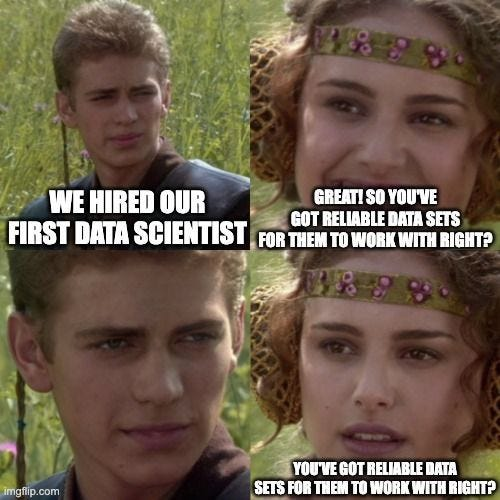
\includegraphics[scale=0.25]{lpu/data.jpeg}
  \label{fig:data}
\end{figure}

\end{hinweis}

Falls Sie diese Unterlagen nicht im Klassenverband bearbeiten, können Sie die nachfolgende Aufgabe überspringen und stattdessen \href{https://www.kaggle.com/datasets/burnoutminer/heights-and-weights-dataset}{diesen}\footnote{\href{https://www.kaggle.com/datasets/burnoutminer/heights-and-weights-dataset}{\url{kaggle.com/datasets/burnoutminer/heights-and-weights-dataset}}} Datensatz verwenden. Allerdings müssten Sie dort die Grössen von \textit{inches} in Zentimeter und Pfund in Kilogramm umrechnen.

\begin{aufgabe}{2: Datensammlung}
Erstellen Sie einen Datensatz mit Grösse und Gewicht Ihrer Klassenkameradinnen und -kameraden. Da es nur darum geht, anschauliche Daten zu generieren, können Sie hier auch Fantasie-Werte angeben.

\begin{itemize}
  \item Bestimmen Sie in der Klasse eine Person als \emph{Schreiber} und eine als \emph{Untersucher}.
  \item Der Schreiber erstellt eine anonyme Excel-Tabelle, in die die Daten eingetragen werden.
  \item Der Untersucher fragt die Klassenmitglieder individuell nach Grösse und Gewicht, und gibt diese ohne den Namen an den Schreiber weiter.
  \item Der Schreiber teilt den fertigen Datensatz mit der Klasse.
\end{itemize}
\end{aufgabe}

Auch wenn diese Art der Datenbeschaffung mühsam erscheinen mag, so vermittelt sie doch ein Gefühl dafür, wie schwierig es sein kann, an gute Daten zu kommen!

\begin{aufgabe}{3}
\begin{enumerate}
    \item Verwenden Sie Ihre Formel aus der ersten Aufgabe, um für jede Grösse ein Gewicht vorherzusagen. 
    \item Vergleichen Sie Ihre Vorhersagen mit den tatsächlichen Werten.
    \item Wie würden Sie Ihren Klassenkameraden mit einem Zahlenwert zusammenfassen, wie ``korrekt'' Ihre Formel für den ganzen Datensatz liegt? 
    \item Können Sie so die Formel in der Klasse ermitteln, welche am ``besten'' ist?
\end{enumerate}
\end{aufgabe}

Wie Sie vermutlich erkannt haben, müssen Sie die Unterschiede zwischen den Vorhersagen Ihrer Formel und den tatsächlichen Werten verrechnen. Die nachfolgende Darstellung \ref{fig:error} stellt dies schematisch dar.

\begin{figure}[h]
\centering
\begin{tikzpicture}[scale=0.8]
  % Achsen + Raster
  \draw[step=1cm,help lines,draw=gray!20] (0,0) grid (10,7);
  \draw[->,thick] (0,0) -- (10.6,0) node[below] {$x$};
  \draw[->,thick] (0,0) -- (0,7.4) node[left] {$y$};

  % Regressionsgerade: y = 0.6 x + 1
  \draw[very thick,blue] (0,1) -- (10,7)

  % Hilfsfunktion: Vorhersagewert auf der Geraden (nur visuell, hier direkt als Koordinaten genutzt)
  % Datenpunkte (x,y)
  % und zugehoerige Vorhersage y_hat = 0.6*x + 1 fuer die Residuen
  % Punkt 1
  \fill[black] (1,1.8) circle (2.2pt);
  \draw[red!70,thick] (1,1.8) -- (1,1.6); % Residuum
  % Punkt 2
  \fill[black] (2,2.5) circle (2.2pt);
  \draw[red!70,thick] (2,2.5) -- (2,2.2);
  % Punkt 3
  \fill[black] (3,2.7) circle (2.2pt);
  \draw[red!70,thick] (3,2.7) -- (3,2.8);
  % Punkt 4
  \fill[black] (5,4.1) circle (2.2pt);
  \draw[red!70,thick] (5,4.1) -- (5,4.0);
  % Punkt 5 (bewusst groesseres Residuum)
  \fill[black] (7,4.2) circle (2.2pt);
  \draw[red!70,thick] (7,4.2) -- (7,5.2);
  % Punkt 6
  \fill[black] (9,6.8) circle (2.2pt);
  \draw[red!70,thick] (9,6.8) -- (9,6.4);

\end{tikzpicture}
\caption{Visualisierung des Unterschieds zwischen Vorhersage mittels linearer Regression und tatsächlichen Datenpunkten.}
\label{fig:error}

\end{figure}


Hierzu gibt es unterschiedliche Methoden, wie man mit den oben \textcolor{red!70}{rot} dargestellten Unterschieden verrechnen könnte. Man könnte sie zum Beispiel summieren, aber wir verwenden in dieser Unterrichtseinheit folgenden Ansatz:

\begin{theorie}
    Die \textbf{mittlere quadratische Abweichung} (\textit{mean squared error} zu Englisch, \textit{MSE} abgekürzt) ist ein Fehlermass, also eine Art, auszudrücken, wie hoch der Fehler einer \textit{Regression} über einem Datensatz im Vergleich zu den tatsächlichen Werten ist.

     \[
  \text{MSE} = \frac{1}{n} \sum_{i=1}^{n} \left( \text{tatsächlich}_{i} - \text{vorhergesagt}_{i} \right)^2
  \]

  Zu Deutsch ist der MSE der Durchschnitt der quadrierten Unterschiede. Wir nehmen das Quadrat der Unterschiede, da uns im MSE nicht interessiert, ob unser Modell unter oder über dem eigentlichen Wert liegt, sondern lediglich um \textit{wieviel} daneben es liegt. Je kleiner der MSE, umso näher liegt das Modell an den tatsächlichen Daten.
\end{theorie}


Wir berechnen nun den MSE anhand eines Beispiels gemeinsam.

Nehmen wir die Punkte aus der obigen Grafik. Für diese sechs Punkte messen wir die Abstände zu der Vorhersage, also die senkrechten Abstände zur Geraden. Damit man es leichter nachrechnen kann, runden wir die Abstände hier auf einfache Zahlen:

\[
e_1 = 0.2,\quad e_2 = 0.3,\quad e_3 = -0.1,\quad e_4 = 0.1,\quad e_5 = -1.0,\quad e_6 = 0.4
\]

Die Vorzeichen (plus oder minus) zeigen nur an, ob ein Punkt oberhalb oder unterhalb der Geraden liegt. Für den MSE interessiert uns aber nur die Grösse des Fehlers, nicht die Richtung. Darum quadrieren wir die Werte:

\[
e_1^2 = 0.04,\quad e_2^2 = 0.09,\quad e_3^2 = 0.01,\quad e_4^2 = 0.01,\quad e_5^2 = 1.00,\quad e_6^2 = 0.16
\]

Jetzt summieren wir alle quadrierten Werte:

\[
0.04 + 0.09 + 0.01 + 0.01 + 1.00 + 0.16 = 1.31
\]

Schliesslich teilen wir diese Summe durch die Anzahl der Punkte (hier: 6). Damit erhalten wir den MSE:

\[
\text{MSE} = \frac{1.31}{6} \approx 0.22
\]

Der mittlere quadratische Fehler ist hier ungefähr $0.22$. Das ist ein recht kleiner Wert – die Gerade passt also insgesamt nicht schlecht. Wenn wir eine andere Gerade ausprobieren würden, die besser zu den Daten passt, sollte der MSE noch kleiner werden.

Solche Fehlermasse können wir aber nicht nur verwenden, um fertige Modelle zu evaluieren; sondern auch, um bessere Modelle zu erstellen. Dies sehen Sie in der nachfolgenden Aufgabe:

\begin{aufgabe}{4}
    Berechnen Sie für Ihre ursprüngliche Formel aus der Aufgabe 3 den MSE. Davon ausgehend, fangen Sie an, den Koeffizienten Ihrer Formel zu verändern und die Auswirkungen davon auf den MSE zu beobachten. Verändern Sie den Koeffizienten so lange, bis der MSE so klein wie möglich ist.
\end{aufgabe}

Herzlichen Glückwunsch! Sie haben einen entscheidenden Schritt auf Ihrer Reise in der Welt des maschinellen Lernens getätigt!

Wir haben gesehen: Wir suchen eine Gerade, die möglichst gut durch die Punktewolke passt. Wir machen das, indem wir die Fehler messen und dann die Gerade so verschieben, dass der mittlere quadratische Fehler (MSE) möglichst klein wird.

Dieses Vorgehen, also das \textit{Finden einer Linie, die den Zusammenhang zwischen zwei Grössen beschreibt}, nennt man \textbf{Regression}.

Das Wort kommt vom lateinischen \textit{regressio}, was so viel wie ``Rückschritt'' bedeutet. Warum? Weil wir von den einzelnen Messpunkten wieder ``zurückgehen'' zu einer einfacheren, allgemeinen Beziehung: anstatt jeden einzelnen Punkt im Detail zu betrachten, fassen wir die Datenpunkte mit einer einfachen Formel zusammen.

In unserem Beispiel bedeutet das:
\[
\text{Gewicht} \approx \text{Koeffizient} \times \text{Grösse}
\]

Natürlich stimmt diese Formel nicht für jede einzelne Person perfekt. Aber sie gibt uns eine Näherung: Wenn wir nur die Grösse kennen, können wir trotzdem eine Schätzung für das Gewicht machen.

\textbf{Darum spricht man von Regression:} Wir reduzieren viele einzelne Beobachtungen auf eine gemeinsame Regel, die uns erlaubt, Vorhersagen zu machen.


\begin{theorie}
Mit dieser Methode haben Sie ein erstes Regressionsmodell trainiert: Sie haben eine \emph{Modellform} definiert, eine \emph{Fehlerfunktion} (hier den MSE) bestimmt und anschliessend durch Variation die beste Variante davon ermittelt. In der Praxis übernimmt diese Optimierung später eine Software wie \texttt{scikit-learn}.
\end{theorie}

\subsubsection*{Zusammenfassung}

In diesem Kapitel haben Sie gelernt, wie man mithilfe der \textbf{linearen Regression} numerische Vorhersagen trifft.

\begin{itemize}
  \item Bei einer Regression versucht man, einen \textbf{Zusammenhang zwischen zwei Grössen} (z.B. Grösse und Gewicht) zu finden.
  \item Dazu verwendet man eine einfache \textbf{Gerade} der Form:
  \[
  \text{Vorhersage} = \text{Koeffizient} \times \text{Eingabe}
  \]
  \item Um zu beurteilen, wie gut diese Gerade zu den echten Daten passt, verwendet man den \textbf{mittleren quadratischen Fehler} (MSE).  
  \item Der MSE misst den durchschnittlichen Abstand zwischen den vorhergesagten und den tatsächlichen Werten — unabhängig vom Vorzeichen:
  \[
  \text{MSE} = \frac{1}{n} \sum_{i=1}^{n} (\text{tatsächlich}_i - \text{vorhergesagt}_i)^2
  \]
  \item Je kleiner der MSE, desto besser passt das Modell zu den Daten.
  \item Eine \textbf{Regression} ist der Versuch, viele Datenpunkte durch eine einfache Regel zu erklären – sie geht ``zurück'' von vielen Einzelwerten zu einer allgemeinen Beziehung.
\end{itemize}

\subsubsection*{Übungsaufgaben}

\begin{aufgabe}{I}
Stellen Sie sich vor, jemand hat die Formel  
\[
\text{Gewicht} = 0.25 \times \text{Grösse [cm]}
\]  
aufgestellt.  
\begin{itemize}
  \item Berechnen Sie mit dieser Formel das vorhergesagte Gewicht einer Person mit 180 cm Grösse.
  \item Vergleichen Sie die Vorhersage mit einem tatsächlichen Gewicht von 70 kg.  
  \item Wie gross ist der quadratische Fehler in diesem Fall?
\end{itemize}
\end{aufgabe}

\begin{aufgabe}{II}
Ein Modell sagt für 5 Personen folgende Gewichte vorher.  
Vergleichen Sie die Vorhersagen mit den echten Werten und berechnen Sie den MSE.

\begin{center}
\begin{tabular}{|c|c|c|}
\hline
\textbf{Person} & \textbf{Vorhersage (kg)} & \textbf{Tatsächlich (kg)} \\
\hline
1 & 60 & 61 \\
2 & 75 & 76 \\
3 & 58 & 60 \\
4 & 82 & 84 \\
5 & 70 & 67 \\
\hline
\end{tabular}
\end{center}
\end{aufgabe}

\begin{aufgabe}{III}
Warum ist es sinnvoll, den Fehler zu \textbf{quadrieren}, bevor man ihn mittelt? Was wäre das Problem, wenn man einfach die Differenzen aufsummiert?
\end{aufgabe}

    
\end{lpu}



\subsection*{Didaktische Überlegungen}

Dieses Kapitel zur linearen Regression wurde so gestaltet, dass die SuS sowohl ein grundlegendes Verständnis für das Prinzip der Vorhersage numerischer Werte entwickeln als auch einen ersten vollständigen Modellierungsprozess durchlaufen — von der Datensammlung über die Modellformulierung bis hin zur Evaluation. Auf diesem wird später im Sinne eines Spiralkurrikulums aufgebaut.

Ein zentrales didaktisches Anliegen dieser Aufgabe liegt in der bewussten Entscheidung, die SuS ihre eigenen Daten erheben zu lassen. Dies hat mehrere Vorteile:

\begin{itemize}
  \item \textbf{Eigenverantwortung und Datenbewusstsein:} Die SuS erfahren, dass der Erfolg von ML-Algorithmen wesentlich von der Qualität der zugrundeliegenden Daten abhängt. Durch das Erfassen eigener Körperdaten entsteht ein hohes Mass an Identifikation mit dem Datensatz.
  
  \item \textbf{Fehlerquellen reflektieren:} Bei der Erhebung können Diskussionen auftreten, insbesondere über Messfehler, Datenschutz und Standardisierung.
  
  \item \textbf{Intuition des später verwendeten Begriffs der \emph{features}:} Die SuS erkennen, dass sie bewusst entscheiden müssen, welche Informationen (Grösse, Gewicht) in das Modell eingehen sollen.
\end{itemize}

Das gewählte Modell — eine lineare Funktion zwischen Grösse und Gewicht — ist bewusst stark vereinfacht. Im Plenum kann diskutiert werden, wie sich das Modell verbessern liesse:

\begin{itemize}
  \item \textbf{Einbezug weiterer Merkmale:} Das Geschlecht könnte als weiterer Prädiktor (\texttt{feature}) berücksichtigt werden. Dies führt zur \emph{multiplen linearen Regression} und erlaubt eine differenziertere Vorhersage.
  
  \item \textbf{Nichtlineare Zusammenhänge:} Die SuS könnten vermuten, dass die Beziehung zwischen Grösse und Gewicht nicht vollständig linear ist. Diese Hypothese eröffnet eine Diskussion über quadratische Modelle oder andere Regressionsformen.
  
  \item \textbf{Visualisierung und Streuung:} Durch die Darstellung als Streudiagramm wird ersichtlich, dass ein Modell nie alle Werte exakt trifft. Die SuS erkennen so die Bedeutung des MSE als \emph{Fehlermass}, aber auch seine Grenzen (z.B. Empfindlichkeit gegenüber Ausreissern).
\end{itemize}

\subsection*{Musterlösungen}

\begin{aufgabe}{1}
Die Fragestellung zielt auf ein erstes, noch rein heuristisches Modell ab. 
Die SuS sollen versuchen, eine Formel der Form
\[
\text{Gewicht [kg]} = \text{Koeffizient} \times \text{Grösse [cm]}
\]
aufzustellen. Die Idee ist, dass grössere Personen tendenziell schwerer sind. 
Ein erster Versuch könnte sein:
\[
\text{Gewicht [kg]} = 0.5 \,\frac{\text{kg}}{\text{cm}} \times \text{Grösse [cm]}
\]
Für eine Person mit \(170\,\text{cm}\) ergibt dies:
\[
\text{Gewicht [kg]} = 0.5 \,\frac{\text{kg}}{\text{cm}} \times 170\,\text{cm} = 85\,\text{kg}
\]
Dies erscheint leicht zu hoch. Mit einem kleineren Koeffizienten, 
z.\,B. \(0.38\,\tfrac{\text{kg}}{\text{cm}}\):
\[
\text{Gewicht [kg]} = 0.38 \,\frac{\text{kg}}{\text{cm}} \times 170\,\text{cm} 
\approx 64.6\,\text{kg}
\]
Diese Formel ist realistischer. Eine brauchbare Startschätzung für viele Personen 
könnte daher sein:
\[
\boxed{\text{Gewicht [kg]} \approx 0.4 \,\frac{\text{kg}}{\text{cm}} \times \text{Grösse [cm]}}
\]
\end{aufgabe}


\begin{aufgabe}{2 und 3}
Die Umrechnung der Daten aus den Beispiel-Datensatz sowie die Formeln zur Berechnung des MSE im Excel sind in der beiliegenden Datei \texttt{LA\_1607\_L.xlsx} zu finden.

Beispielrechnung für 3 Datenpunkte:
\begin{align*}
\text{MSE} &= \frac{1}{3} \left[(85 - 0.4 \cdot 182)^2 + (66 - 0.4 \cdot 168)^2 + (87 - 0.4 \cdot 188)^2 \right] \\
&= \frac{1}{3} \left[(12.2)^2 + (-1.2)^2 + (11.8)^2\right] \\
&= \frac{1}{3} (148.84 + 1.44 + 139.24) = \boxed{96.51}
\end{align*}
\end{aufgabe}

\begin{aufgabe}{I}
\begin{itemize}
  \item $0.25 \times 180 = 45$ kg  
  \item Tatsächliches Gewicht = 70 kg → Differenz = $70 - 45 = 25$
  \item Quadratischer Fehler = $25^2 = 625$
\end{itemize}
\end{aufgabe}

\begin{aufgabe}{II}
\[
\begin{aligned}
(60 - 61)^2 &= 1 \\
(75 - 76)^2 &= 1 \\
(58 - 60)^2 &= 4 \\
(82 - 84)^2 &= 4 \\
(70 - 67)^2 &= 9 \\
\text{Summe} &= 19,\quad \text{MSE} = \frac{19}{5} = 3.8
\end{aligned}
\]
\end{aufgabe}

\begin{aufgabe}{III}
Wenn man die Fehler einfach aufsummiert, könnten sich positive und negative Abweichungen gegenseitig aufheben. So könnte der Durchschnittsfehler null sein, obwohl die Vorhersagen schlecht sind.  
Durch das Quadrieren wird jede Abweichung positiv und grosse Fehler zählen stärker.
\end{aufgabe}

\subsection{Ballung}
\label{sec:clustering}
\begin{lpu}{Wie man ähnliche Dinge zu Gruppen zusammenfasst: Ballung}

Nachdem Sie bereits zwei Arten von Algorithmen des maschinellen Lernens kennengelernt haben — einen für die Klassifikation (nämlich den Entscheidungsbaum) und die lineare Regression für numerische Vorhersagen — begegnet Ihnen nun eine dritte: die \textbf{Ballung}, auch \emph{clustering} genannt. Während bei der Entwicklung für Algorithmen der Klassifikation und Regression jeweils die \emph{richtige Antwort} vorgegeben ist (man spricht von \emph{überwachtem Lernen}), ist dies bei Ballung nicht der Fall: Sie erkennen Strukturen in Daten, ohne dass jemand vorher gesagt hat, wie viele Gruppen es gibt oder wie diese aussehen sollen.

Ein typisches Beispiel: Ein Onlineshop möchte seine Kundschaft segmentieren, um gezieltere Werbung zu machen. Dazu werden Merkmale wie Bestellverhalten oder Preisempfindlichkeit betrachtet – ohne zu wissen, wie viele «Typen» von Kundinnen und Kunden es gibt. Stellen Sie sich also vor, Sie betrieben einen Online-Shop für Elektronik. In Ihrem System liegen Daten vor über alle Bestellungen der letzten zwei Jahre: Wie teuer war die Bestellung? Zu welcher Tageszeit wurde sie getätigt? Welche Produktkategorien waren beteiligt? Nun möchten Sie Ihre Kundschaft \textit{segmentieren} (also in Gruppen einteilen), um gezieltere Angebote zu machen:

Sie möchten für diese Gruppen unterschiedliche Rabatte oder Newsletter formulieren – wissen aber nicht im Voraus, wie viele Gruppen existieren oder wie diese genau definiert sind. Hier kommt ein Ballungsalgorithmus ins Spiel: Er gruppiert die vorhandenen Daten in sinnvolle \textit{cluster} (= Gruppen), basierend auf Ähnlichkeiten zwischen ihnen.

Ein anderes Beispiel: Stellen Sie sich vor, Spotify möchte auswerten, wie sich verschiedene Nutzerinnen und Nutzer verhalten. Jede Person hört unterschiedlich oft Musik, zu verschiedenen Tageszeiten, in verschiedenen Genres. Spotify kann diese Daten verwenden, um Nutzerinnen und Nutzer automatisch in Gruppen einzuteilen und für diese Gruppen geeignete Vorschläge zu machen. Beispielsweise könnte ein Ballungs-Algorithmus automatisch herausfinden, dass es folgende Gruppen gibt:

\begin{itemize}
  \item Lernende, die tagsüber ruhige Musik hören.
  \item Sportlich Aktive, die vorwiegend Beats am Abend hören.
  \item Gelegenheitshörerinnen, die ab und zu einen Hit-Remix streamen.
\end{itemize}

Wichtig zu verstehen ist, dass hier niemand \textit{a priori} sagt, dass es diese Kategorien gibt, sondern sich diese aus den Daten direkt ergeben. 

\begin{theorie}
Dies nennt man \textbf{unüberwachten Lernen} (\emph{unsupervised learning}). Hier versucht ein Algorithmus, Strukturen oder Muster in einem Datensatz zu erkennen, \textbf{ohne dass richtige Antworten vorgegeben sind}. Es gibt also keine Labels, keine Zielwerte. Stattdessen werden Ähnlichkeiten in den Daten genutzt, um Gruppen (\textit{cluster}), Ausreisser oder Ordnungen zu finden. Diese Algorithmen sind nützlich, wenn Sie in Daten verborgene Strukturen aufdecken wollen, ohne vorab zu wissen, welche Kategorien es gibt.
\end{theorie} 


\begin{aufgabe}{1}
Lesen Sie den folgenden Absatz und beantworten Sie anschliessend die Fragen:

\emph{Stellen Sie sich nun vor, Sie betrieben einen solchen Onlinehandel, wie oben beschrieben, selber. In Ihrem Kundenstamm gibt es verschiedene Typen: Einige kaufen spontan und achten stark auf Preisaktionen. Andere planen ihren Einkauf langfristig, aber kaufen bevorzugt Premiumprodukte. Vermutlich gibt es aber auch noch viele andere Typen! Wenn Sie Kunden der jeweiligen Typen unterschiedliche Angebote machen könnten – wie würden Sie herausfinden, wie viele Gruppen es gibt, und wer zu welcher gehört?}

\begin{itemize}
  \item Warum sind in dieser Situation keine Kategorien im Voraus bekannt?
  \item Warum kann ein Entscheidungsbaum hier nicht angewendet werden?
  \item Welche Vorteile könnte es haben, solche Gruppen automatisch zu erkennen?
\end{itemize}
\end{aufgabe}

Wir wechseln nun das Beispiel zum letzten Mal, und nehmen zur Hand das Parade-Beispiel für die Ballung: Sie besitzen eine Kette von Pizza-Kurieren, welche in einer grossen Stadt mehrere Standorte haben. Nachfolgend finden Sie eine Grafik, wo die meisten Bestellungen getätigt werden. 

\begin{figure}[h]
\centering
\begin{tikzpicture}[scale=0.4]
\draw[step=1cm,gray,very thin] (0,0) grid (20,20);
\draw[->] (0,0) -- (21,0) node[right] {$x$};
\draw[->] (0,0) -- (0,21) node[above] {$y$};

\filldraw[black] (5.50,14.86) circle (2pt);
\filldraw[black] (5.65,16.52) circle (2pt);
\filldraw[black] (4.77,14.77) circle (2pt);
\filldraw[black] (6.58,15.77) circle (2pt);
\filldraw[black] (4.53,15.54) circle (2pt);
\filldraw[black] (4.54,14.53) circle (2pt);
\filldraw[black] (5.24,13.09) circle (2pt);

\filldraw[black] (13.28,14.44) circle (2pt);
\filldraw[black] (13.99,15.31) circle (2pt);
\filldraw[black] (14.09,13.59) circle (2pt);
\filldraw[black] (16.47,14.77) circle (2pt);
\filldraw[black] (15.07,13.58) circle (2pt);
\filldraw[black] (14.46,15.11) circle (2pt);
\filldraw[black] (13.85,15.38) circle (2pt);

\filldraw[black] (9.40,4.71) circle (2pt);
\filldraw[black] (9.40,6.85) circle (2pt);
\filldraw[black] (9.99,3.94) circle (2pt);
\filldraw[black] (10.82,3.78) circle (2pt);
\filldraw[black] (10.21,3.04) circle (2pt);
\filldraw[black] (8.67,5.20) circle (2pt);
\filldraw[black] (10.74,5.17) circle (2pt);

% Aufgabe: Tragen Sie hier Ihre drei Depot-Standorte ein, z.B.:
% \filldraw[red] (x,y) node[below right]{Depot 1} circle (4pt);

\end{tikzpicture}
\caption{Bestellungen als Punkte im Stadtgebiet}
\label{fig:pizza_kmeans_example}
\end{figure}

Da Sie wissen, dass das Geheimnis des Erfolges Ihres Unternehmens darin liegt, dass die Pizza so nah wie möglich an Ihren Kunden produziert wird (um schnelle Lieferzeiten und eine höhere Knusprigkeit des Pizzarandes zu gewährleisten), möchten Sie neue Standorte aufbauen, die möglichst nah an möglichst vielen Kunden liegen. Im Beispiel oben ist das nicht schwierig, aber wie sieht es im nachfolgenden Beispiel aus?

\begin{figure}[h]
\centering
\begin{tikzpicture}[scale=0.4]
\draw[step=1cm,gray,very thin] (0,0) grid (20,20);
\draw[->] (0,0) -- (21,0) node[right] {$x$};
\draw[->] (0,0) -- (0,21) node[above] {$y$};

\filldraw[black] (1.61,18.19) circle (2pt);
\filldraw[black] (4.62,12.69) circle (2pt);
\filldraw[black] (2.73,19.63) circle (2pt);
\filldraw[black] (1.34,15.06) circle (2pt);
\filldraw[black] (6.79,14.09) circle (2pt);
\filldraw[black] (2.51,15.79) circle (2pt);
\filldraw[black] (7.28,14.59) circle (2pt);

\filldraw[black] (15.02,15.04) circle (2pt);
\filldraw[black] (19.85,18.81) circle (2pt);
\filldraw[black] (18.21,16.85) circle (2pt);
\filldraw[black] (17.62,19.28) circle (2pt);
\filldraw[black] (13.94,18.59) circle (2pt);
\filldraw[black] (13.24,14.60) circle (2pt);
\filldraw[black] (18.00,12.86) circle (2pt);

\filldraw[black] (9.69,0.10) circle (2pt);
\filldraw[black] (9.44,4.16) circle (2pt);
\filldraw[black] (6.10,0.46) circle (2pt);
\filldraw[black] (12.04,1.62) circle (2pt);
\filldraw[black] (10.01,3.51) circle (2pt);
\filldraw[black] (8.07,2.62) circle (2pt);
\filldraw[black] (8.23,1.80) circle (2pt);

% Aufgabe: Tragen Sie hier Ihre drei Depot-Standorte ein, z.B.:
% \filldraw[red] (x,y) node[below right]{Depot 1} circle (4pt);

\end{tikzpicture}
\caption{Verstreut liegende Pizzabestellungen}
\label{fig:pizza_kmeans_variante}
\end{figure}

\begin{aufgabe}{2a}
In Abbildung~\ref{fig:pizza_kmeans_variante} sehen Sie also die Positionen von Pizzabestellungen in einer Stadt. Die Punkte sind diesmal deutlich unregelmässiger verteilt als im vorherigen Beispiel. Sie möchten drei neue Depots eröffnen, von denen die Pizzas geliefert werden. Ziel ist es, dass:

\begin{itemize}
  \item jede Bestellung möglichst nah bei einem Depot liegt,
  \item die Depots möglichst gleichmässig ausgelastet sind.
\end{itemize}

\vspace{1em}
\textbf{1. Gruppieren Sie von Hand}

\begin{itemize}
  \item Versuchen Sie, die Punkte visuell in drei Gruppen zu unterteilen.
  \item Zeichnen Sie mit Farbstiften oder Markierungen ein, welche Punkte Sie jeweils zusammenfassen würden.
  \item Überlegen Sie: Was macht eine ``gute'' Gruppe aus?
\end{itemize}

\vspace{1em}
\textbf{2. Wählen Sie Gruppenzentren}

\begin{itemize}
  \item Bestimmen Sie für jede Gruppe ein Zentrum (einen ``günstigen'' Ort für ein Depot).
  \item Notieren Sie sich die Koordinaten der Zentren.
  \item Warum haben Sie genau diese Punkte gewählt?
\end{itemize}
\end{aufgabe}

In dieser Aufgabe haben Sie die Gruppen intuitiv gebildet. Doch wie bringen Sie einem Computer bei, automatisch solche Gruppierungen zu finden? Die nächsten zwei Teilaufgaben führen Sie dazu hin, zu verstehen, wie man algorithmisch solche Gruppen und Zentren finden kann.


\begin{aufgabe}{2b}
Wenn Sie die Gruppierungen aus Aufgabe 2a ``vergessen'', aber die Zentren beibehalten. Die nachfolgende Darstellung hilft Ihnen beim Visualisieren, aber Sie können auch \textit{Ihre} Zentren verwenden.

\begin{center}
\begin{tikzpicture}[scale=0.4]
\draw[step=1cm,gray,very thin] (0,0) grid (20,20);
\draw[->] (0,0) -- (21,0) node[right] {$x$};
\draw[->] (0,0) -- (0,21) node[above] {$y$};

\filldraw[black] (1.61,18.19) circle (2pt);
\filldraw[black] (4.62,12.69) circle (2pt);
\filldraw[black] (2.73,19.63) circle (2pt);
\filldraw[black] (1.34,15.06) circle (2pt);
\filldraw[black] (6.79,14.09) circle (2pt);
\filldraw[black] (2.51,15.79) circle (2pt);
\filldraw[black] (7.28,14.59) circle (2pt);

\filldraw[black] (15.02,15.04) circle (2pt);
\filldraw[black] (19.85,18.81) circle (2pt);
\filldraw[black] (18.21,16.85) circle (2pt);
\filldraw[black] (17.62,19.28) circle (2pt);
\filldraw[black] (13.94,18.59) circle (2pt);
\filldraw[black] (13.24,14.60) circle (2pt);
\filldraw[black] (18.00,12.86) circle (2pt);

\filldraw[black] (9.69,0.10) circle (2pt);
\filldraw[black] (9.44,4.16) circle (2pt);
\filldraw[black] (6.10,0.46) circle (2pt);
\filldraw[black] (12.04,1.62) circle (2pt);
\filldraw[black] (10.01,3.51) circle (2pt);
\filldraw[black] (8.07,2.62) circle (2pt);
\filldraw[black] (8.23,1.80) circle (2pt);

\filldraw[red] (4,16) node[below right]{Zentrum 1} circle (4pt);
\filldraw[red] (17,17) node[below right]{Zentrum 2} circle (4pt);
\filldraw[red] (9,2) node[below right]{Zentrum 3} circle (4pt);

\end{tikzpicture}
\end{center}


Wenn Sie ein Computer wären: Wie würden Sie für einen gegebenen Punkt entscheiden, welchem Zentrum er zugeordnet werden sollte?
\end{aufgabe}

\begin{aufgabe}{2c}
Drehen wir den Spiess um: Wir ``vergessen'' die Zentren, aber merken uns die Gruppierung:

\centering
\begin{tikzpicture}[scale=0.4]
  % Achsen und Gitter
  \draw[step=1cm,gray,very thin] (0,0) grid (20,20);
  \draw[->] (0,0) -- (21,0) node[right] {$x$};
  \draw[->] (0,0) -- (0,21) node[above] {$y$};

  % Gruppe 1 (links oben, blau)
  \foreach \x/\y in {1.61/18.19, 4.62/12.69, 2.73/19.63, 1.34/15.06,
                     6.79/14.09, 2.51/15.79, 7.28/14.59}{
    \filldraw[blue] (\x,\y) circle (3pt);
  }

  % Gruppe 2 (rechts oben, grün)
  \foreach \x/\y in {15.02/15.04, 19.85/18.81, 18.21/16.85, 17.62/19.28,
                     13.94/18.59, 13.24/14.60, 18.00/12.86}{
    \filldraw[green!70!black] (\x,\y) circle (3pt);
  }

  % Gruppe 3 (unten, orange)
  \foreach \x/\y in {9.69/0.10, 9.44/4.16, 6.10/0.46, 12.04/1.62,
                     10.01/3.51, 8.07/2.62, 8.23/1.80}{
    \filldraw[orange] (\x,\y) circle (3pt);
  }

\end{tikzpicture}

Wie würden Sie als Computer für jede Gruppe das Zentrum berechnen?

\end{aufgabe}

Sie haben gerade selbst die Grundidee des \textbf{\textit{k-means}-Algorithmus} entdeckt – ein Verfahren, das Gruppen findet, indem es immer wieder Gruppenzugehörigkeiten aktualisiert und neue Gruppenzentren berechnet. Während Sie sich hier noch auf Ihre Intuition verlassen haben, um die ersten Gruppierungen und Zentren zu bestimmen, verfügt ein Computer nicht über eine Intuition. An deren Stelle rücken der Zufall und die Iteration. 


\begin{aufgabe}{3}
Benutzen Sie \href{https://www.naftaliharris.com/blog/visualizing-k-means-clustering/}{diese Simulation}\footnote{\href{https://www.naftaliharris.com/blog/visualizing-k-means-clustering/}{\url{naftaliharris.com/blog/visualizing-k-means-clustering/}}}, um sich ein Bild davon zu machen, wie \textit{k-means} funktioniert. Beginnen Sie dort mit \tikz[baseline=(X.base)]
  \node[draw=black, rounded corners, inner xsep=2pt, inner ysep=1pt]
  (X) {\textsf{Randomly}}; für \textit{How to pick the initial centroids?}; dann wählen Sie zunächst \tikz[baseline=(X.base)]
  \node[draw=black, rounded corners, inner xsep=2pt, inner ysep=1pt]
  (X) {\textsf{Gaussian Mixture}};. Spielen Sie im Anschluss mit verschiedene Einstellungen!


\vspace{0.5em}
Beantworten Sie danach folgende Fragen:

\begin{itemize}
  \item Was passiert, wenn zwei Zentren sehr nahe beieinander liegen? (Dazu können Sie zu Beginn der Simulation \tikz[baseline=(X.base)]
  \node[draw=black, rounded corners, inner xsep=2pt, inner ysep=1pt]
  (X) {\textsf{I'll Choose}}; wählen.)
  \item Wie verhält sich der Algorithmus bei ``nicht-runden'' Gruppenformen?
  \item Ist die Wahl der Startpunkte wichtig?
\end{itemize}
\end{aufgabe}

Dieses Vorgehen wird nun mathematisch formalisiert.

\begin{theorie}
Ein verbreiteter Algorithmus zur Ballung ist \textbf{\textit{k-means}}. Er teilt Datenpunkte in genau $k$ Gruppen (Ballungen), sodass jeder Punkt zu dem Zentrum gehört, zu dem er die kleinste Distanz hat.

Die Schritte des Algorithmus:
\begin{enumerate}
  \item Wähle $k$ zufällige Punkte als Start-Zentren.
  \item Ordne jeden Datenpunkt dem nächsten Zentrum zu ($\Rightarrow$ erste Ballungen).
  \item Berechne für jede Ballung den Mittelpunkt (\textit{Zentroid}).
  \item Wiederhole Schritt 2–3, bis sich die Zentren nicht mehr (viel) verändern.
\end{enumerate}

Die Distanz zwischen Datenpunkten $x$ und $c$ wird dabei durch die \textbf{euklidische Distanz} gemessen:
\[
\text{dist}(p, c) = \sqrt{(p^{(x)} - c^{(x)})^2 + (p^{(y)} - c^{(y)})^2}
\]

Allgemein (für $d$ Dimensionen):
\[
\text{dist}(p, c) = \sqrt{ \sum_{i=1}^d (p^{(i)} - c^{(i)})^2 }
\]

Sobald alle Punkte einer Gruppe zugewiesen sind, wird für jede Gruppe $G_j$ ein neues Gruppenzentrum (Zentroid) $c_j$ (wie \textit{centroid}) berechnet – als \textbf{Mittelwert} aller Punkte in dieser Gruppe.

\vspace{0.5em}
\textbf{Berechnung des Gruppenzentrums (Zentroid)}

Für jede Gruppe \( G_j \) mit Punkten \( x_1, x_2, \dots, x_n\) berechnet man das neue Zentrum \( c_j\) indem jede Koordinate separat gemittelt wird:

\[
c_j^{(k)} = \frac{1}{|G_j|} \sum_{x_i \in G_j} x_i^{(k)} \quad \text{für } k = 1, 2, \dots, d
\]

Der vollständige Zentroid ergibt sich also als:
\[
c_j = \left( \frac{1}{|G_j|} \sum_{x_i \in G_j} x_i^{(1)},\ 
             \frac{1}{|G_j|} \sum_{x_i \in G_j} x_i^{(2)},\ 
             \dots,\ 
             \frac{1}{|G_j|} \sum_{x_i \in G_j} x_i^{(d)} \right)
\]

Das heisst: Jede Koordinate des Zentroids ist der Mittelwert der entsprechenden Koordinaten aller Punkte der Gruppe.
\end{theorie}

Auch wenn das mathematisch involviert scheinen mag, so ist der Algorithmus einfach zu verstehen. Obwohl Sie für gewöhnlich sich diese Berechnungen von einem Computer ausführen lassen (wie wir später auch sehen werden), ist es lehrreich, wenn Sie einmal zumindest die Berechnung mit Ihrem eigenen Gehirn ausführen.

\begin{aufgabe}{4}
In dieser Aufgabe wenden Sie den \textit{k-means}-Algorithmus auf ein ganz kleines Beispiel in zwei Dimensionen an. Die Punkte sind:

\[
A = (2, 2),\quad B = (3, 4),\quad C = (5, 3),\quad D = (8, 7)
\]

\begin{center}
\begin{tikzpicture}[scale=0.8]
  \draw[step=1cm,gray,very thin] (0,0) grid (10,10);
  \draw[->] (0,0) -- (10.5,0) node[right] {$x$};
  \draw[->] (0,0) -- (0,10.5) node[above] {$y$};

  % Datenpunkte
  \filldraw[black] (2,2) circle (2pt) node[above right] {A};
  \filldraw[black] (3,4) circle (2pt) node[above right] {B};
  \filldraw[black] (5,3) circle (2pt) node[above right] {C};
  \filldraw[black] (8,7) circle (2pt) node[above right] {D};

  % Startzentren
  % \draw[red, thick] (2,2) node[below left] {\textcolor{red}{$Z_1^{(0)}$}} node[cross, red, thick, minimum size=8pt] {};
  % \draw[red, thick] (8,7) node[below right] {\textcolor{red}{$Z_2^{(0)}$}} node[cross, red, thick, minimum size=8pt] {};

\end{tikzpicture}
\end{center}

Wir möchten die Punkte in $k = 2$ Gruppen einteilen.

\begin{enumerate}
  \item \textbf{Start:} Wählen Sie zwei Startzentren ``zufällig''.

  \item \textbf{Zuweisungsschritt:} Berechnen Sie für jeden Punkt der 4 Punkte die euklidische Distanz zu beiden Zentren und ordnen Sie ihn dem nächstgelegenen Startzentrum zu.

  \item \textbf{Zentroid-Schritt:} Berechnen Sie für jede Gruppe den neuen Mittelpunkt (Zentroid) als arithmetischen Mittelwert der Punkte.

  \item \textbf{Wiederholen:} Führen Sie einen weiteren Zuweisungsschritt mit den neuen Zentren durch. Ändern sich die Gruppen? Falls nein: Der Algorithmus ist fertig! Falls ja: Fangen Sie bei Schritt 2. wieder an, und beobachten Sie, wie sich die Zentroide und Gruppen verändern.

\end{enumerate}
\end{aufgabe}


Wenn man ein Verfahren wie \textit{k-means} verwendet, stellen sich drei grundlegende Fragen:

\begin{enumerate}
    \item \textbf{Wie viele Gruppen (\textit{k}) soll man verwenden}
    Die Anzahl \textit{k} muss im klassischen \textit{k-means}-Verfahren vorab gewählt werden. Es gibt keine ``richtige'' Zahl — vielmehr hängt die Wahl davon ab, wie fein oder grob die Gruppierung sein soll.  In der Praxis nutzt man oft sogenannte \textit{elbow plots}, um eine gute Wahl für \textit{k} zu finden: Man berechnet für verschiedene Werte von \textit{k} die Summe der quadratischen Abstände der Punkte zu ihren Gruppenzentren. Diese Summe nimmt mit grösserem \textit{k} ab – aber ab einem bestimmten Punkt lohnt sich das Hinzufügen weiterer Gruppen kaum mehr. Dort ist der ``Knick'' (engl. \textit{elbow}) – ein sinnvoller Kandidat für \textit{k}. Aber das ist nur eine Art, und oft hängt \textit{k} von der Anwendung ab.
    
    \item \textbf{Wann ist das Verfahren fertig?} 
Das Verfahren wird so lange wiederholt , bis sich die Gruppenzentren \textit{kaum} mehr verändern. Aber was heisst \textit{kaum}? In der Praxis kann man z.B. eine Grenze $\varepsilon$ setzen:  
\[
\text{Stopp, wenn sich alle Zentren um weniger als } \varepsilon \text{ verschieben.}
\]

Für $\varepsilon$ gibt es keinen universell richtigen Wert, aber er sollte sich an der Grösse des Datenraumes orientieren. Programmier-Bibliotheken wie \texttt{scikit-learn}, welches Sie später benutzen werden, verwendet $\varepsilon = 10^{-4}$ für normalisierte Daten, bei welchen die Dimensionen zwischen $[0,1]$ liegen. Für unsere Koordinaten sollte der Wert entsprechend höher liegen. Ein anderer Ansatz ist es, eine maximale Anzahl Durchläufe vorgeben (z. B. 100 Wiederholungen).

\item \textbf{Was bedeuten die Gruppen eigentlich?} Eine Frage, die sich beim Entdecken von Gruppen ebenfalls stellt, betrifft deren ``Identität'':  Was genau macht eine Gruppe aus? Was haben die Punkte darin gemeinsam?  

Ein Ballungs-Verfahren kann nur sagen, \emph{dass} Punkte ähnlich sind — nicht \emph{warum}.  
Die Interpretation bleibt Aufgabe der Menschen. Insbesondere bei Datensätzen mit vielen Merkmalen ist es eine echte Herausforderung, eine Gruppe verständlich zu beschreiben:  Welche Eigenschaften teilen die Mitglieder einer Gruppe? Gibt es ein typisches Profil? Manchmal entdeckt ein solcher Algorithmus Ähnlichkeiten, die einem Menschen nicht aufgefallen wären. Aber erklären kann der Algorithmus diese nicht; das bleibt eine menschliche Leistung.
\end{enumerate}

\subsubsection*{Zusammenfassung}

In diesem Kapitel haben Sie den dritten Grundtyp maschinellen Lernens kennengelernt: die \textbf{Ballung} (engl. \textit{clustering}).  

\begin{itemize}
  \item Eine Ballung ist eine Gruppierung von ähnlichen Datenpunkten, ohne dass diese Gruppen vorher vorgegeben sind.
  \item Ballung gehört zum \textbf{unüberwachten Lernen}: Es gibt keine Zielwerte oder Labels – der Algorithmus sucht selbst Strukturen.
  \item Ein bekannter Algorithmus ist \textbf{\textit{k-means}}. Er funktioniert in mehreren Schritten:
    \begin{enumerate}
      \item Starte mit $k$ zufälligen Gruppenzentren.
      \item Ordne alle Punkte dem nächstgelegenen Zentrum zu.
      \item Berechne für jede Gruppe ein neues Zentrum (Zentroid).
      \item Wiederhole, bis sich die Zentren kaum noch verändern.
    \end{enumerate}
  \item Die \textbf{Zugehörigkeit} eines Punktes wird durch die \textbf{Distanz} zum nächsten Zentrum bestimmt.
  \item Die Gruppen, die so entstehen, müssen von Menschen interpretiert werden. Der Algorithmus zeigt nur: \textit{Diese Dinge sind einander ähnlich}.
\end{itemize}


\subsubsection*{Zusammenfassung}

In diesem Kapitel haben Sie den dritten Grundtyp maschinellen Lernens kennengelernt: die \textbf{Ballung} (engl. \textit{clustering}).  

\begin{itemize}
  \item Eine Ballung ist eine Gruppierung von ähnlichen Datenpunkten, ohne dass diese Gruppen vorher vorgegeben sind.
  \item Ballung gehört zum \textbf{unüberwachten Lernen}: Es gibt keine Zielwerte oder Labels – der Algorithmus sucht selbst Strukturen.
  \item Ein bekannter Algorithmus ist \textbf{\textit{k-means}}. Er funktioniert in mehreren Schritten:
    \begin{enumerate}
      \item Starte mit $k$ zufälligen Gruppenzentren.
      \item Ordne alle Punkte dem nächstgelegenen Zentrum zu.
      \item Berechne für jede Gruppe ein neues Zentrum (Zentroid).
      \item Wiederhole, bis sich die Zentren kaum noch verändern.
    \end{enumerate}
  \item Die \textbf{Zugehörigkeit} eines Punktes wird durch die \textbf{Distanz} zum nächsten Zentrum bestimmt.
  \item Die Gruppen, die so entstehen, müssen von Menschen interpretiert werden. Der Algorithmus zeigt nur: \textit{Diese Dinge sind einander ähnlich}.
\end{itemize}

\subsubsection*{Übungsaufgaben}

\begin{aufgabe}{I}
In Ihren Daten liegen Informationen zu Bestellungen vor. Sie kennen aber \textit{keine} Labels (z. B. ``Vielbesteller'' oder ``Gelegenheitshopper'').  
Warum ist Ballung hier ein geeigneter Ansatz? Und warum wäre ein Entscheidungsbaum ungeeignet?
\end{aufgabe}

\begin{aufgabe}{II}
Schreiben Sie in Pseudocode, wie der \texttt{k-means}-Algorithmus funktioniert. Verwenden Sie dabei die Begriffe: \textit{Zentrum}, \textit{Gruppe}, \textit{Distanz}, \textit{Wiederholung} und \textit{Zentroid}.
\end{aufgabe}

\begin{aufgabe}{III}
Sie haben die folgenden Punkte:  
\[
(2, 3),\quad (3, 2),\quad (8, 7),\quad (9, 6)
\]  
Sie starten mit zwei Zentren:  
\[
Z_1 = (2,3),\quad Z_2 = (9,6)
\]

\begin{itemize}
  \item Ordnen Sie jeden Punkt dem näheren Zentrum zu.
  \item Berechnen Sie für jede Gruppe das neue Zentrum (Zentroid).
\end{itemize}
\end{aufgabe}


\end{lpu}

\subsection*{Didaktische Überlegungen}


Das Thema Ballung (\textit{clustering}) stellt eine neue Denkweise im maschinellen Lernen dar: Erstmals arbeiten die SuS mit einem \emph{unüberwachten Verfahren}, bei dem die ``richtigen Antworten'' nicht vorgegeben sind. Statt zwischen Kategorien zu unterscheiden (Klassifikation) oder Werte vorherzusagen (Regression), geht es hier darum, in rohen Daten Muster zu entdecken, ohne dass diese explizit benannt sind. Diese Art des maschinellen Lernens wurde hier bewusst so früh wie möglich eingeführt, damit die SuS ein Konzept vom ML formen, das sowohl überwachtes als auch unüberwachtes Lernen einschliesst, und nicht einen Konzeptwandel vollbringen müssen.

Die vorgeschalteten Aufgaben, in denen SuS Standorte für einen Pizzalieferdienst setzen sollen, bevor der Algorithmus \textit{k-means} überhaupt eingeführt wird, dienen dazu, ein intuitives Verständnis für \textit{cluster} zu entwickeln. Sie lernen, dass Daten sinnvoll gruppiert werden können, auch wenn keine Etikette existiert.

Durch die strukturierte Heranführung an \textit{k-means} – erst durch Ausprobieren, dann durch Theorie, dann durch Visualisieren und zuletzt durch eigenes Berechnen — wird der Algorithmus ``sanft'' eingeführt. Die Verwendung konkreter Koordinaten in der letzten Aufgabe (``\textit{k-means} von Hand durchrechnen'') erlaubt es, das Verfahren schrittweise nachzuvollziehen. Diese Aufgabe ist nicht zwingend erforderlich für alle SuS, kann aber für leistungsstärkere Gruppen eine wertvolle Gelegenheit darstellen, sich mit dem mathematischen Kern des Algorithmus auseinanderzusetzen.

Für schwächere SuS kann diese letzte Aufgabe weggelassen werden, ohne dass das Grundverständnis für Ballungs-Algorithmen verloren geht. Alternativ kann sie als Partner- oder Gruppenarbeit gelöst werden.

\subsubsection*{Mathematische Vertiefung: Vergleich MSE und euklidischer Distanz}

Didaktisch lohnend könnte auch der Vergleich der euklidischen Distanz (im Zuweisungsschritt von \textit{k-means}) mit dem MSE aus dem Kapitel~\ref{sec:regression} sein, der im Zusammenhang  mit der Regression eingeführt wurde. Trotz formaler Ähnlichkeit (beide minimieren summierte quadratische Abstände) verfolgen die beiden Verfahren konzeptionell unterschiedliche Ziele:

\begin{itemize}
  \item Beim MSE werden Fehlerquadrate über \textbf{eine feste Referenz} (z.\,B.\ eine Gerade) berechnet, und der Mittelwert dieser Abweichungen dient der Optimierung.
  \item Beim \textit{k-means} hingegen dient die euklidische Distanz dazu, Punkte \textbf{dynamisch} einem Zentrum zuzuordnen. Die Zentren verändern sich selbst in jedem Schritt.
\end{itemize}

Diese Unterscheidung ist besonders fruchtbar im Hinblick auf Kompetenzaufbau: SuS lernen, dass mathematische Werkzeuge (wie Abstandsmasse) je nach Kontext unterschiedliche Bedeutungen und Funktionen erhalten können.


\subsection*{Musterlösungen}

\begin{aufgabe}{1}
\begin{itemize}
  \item \textbf{Warum sind in dieser Situation keine Kategorien im Voraus bekannt?}

    In dieser Situation liegen keine vordefinierten Labels oder Klassen vor, wie zum Beispiel ``Typ A'' oder ``Typ B''. Es handelt sich um \textbf{Verhaltensmuster}, die sich aus vielen Einzelinformationen (z.\,B.\ Kaufhäufigkeit, Produkttyp, Zeitpunkt, Rabattnutzung) ergeben. Welche Kundentypen überhaupt existieren, ist unbekannt – sie müssen erst aus den Daten erschlossen werden.

    In der Fachsprache handelt es sich deshalb um ein \textbf{unüberwachtes Lernproblem} (\textit{unsupervised learning}), weil keine ``richtigen Antworten'' als Trainingsdaten gegeben sind.

  \item \textbf{Warum kann ein Entscheidungsbaum hier nicht angewendet werden?}

Entscheidungsbäume gehören zum \textbf{überwachten Lernen}. Sie benötigen für jeden Eintrag im Datensatz ein sogenanntes ``Label'' – also eine Zielkategorie, die vom Modell gelernt werden soll (z.\,B.\ ``Kundentyp A''). In unserem Fall liegen jedoch keine solchen vorgegebenen Gruppen vor: Wir wissen nicht, wie viele Typen es gibt, und wir haben keine Information darüber, welcher Kunde zu welcher Gruppe gehört. Deshalb ist ein Entscheidungsbaum hier nicht einsetzbar.

\textbf{Wichtig:} Das Problem liegt \emph{nicht} an der Art der Eingangsdaten. Sowohl Entscheidungsbäume als auch Ballungs-Verfahren wie \textit{k-means} können grundsätzlich mit numerischen und kategorischen Daten umgehen (z.\,B.\ ``bestellt häufig'', ``Zahlungsart = Kreditkarte'', ``durchschnittlicher Warenkorbwert''). Entscheidend ist allein, ob es ein bekanntes Zielattribut (Label) gibt. In unserem Fall fehlt dieses – und deshalb ist ein \textbf{unüberwachter Lernalgorithmus} erforderlich.


  \item \textbf{Welche Vorteile könnte es haben, solche Gruppen automatisch zu erkennen?}

    Die automatische Gruppierung der Kundinnen und Kunden bringt mehrere Vorteile:
    \begin{itemize}
  \item \textbf{Personalisierte Angebote:} Verschiedene Gruppen können gezielt mit passenden Aktionen oder Produktempfehlungen angesprochen werden (z.\,B.\ Rabattgutscheine für preisbewusste Käuferinnen und Käufer, exklusive Neuheiten für Premiumkundschaft).

  \item \textbf{Besseres Kundenverständnis:} Der Algorithmus kann Muster aufdecken, die für Menschen nicht unmittelbar erkennbar sind. Dadurch entsteht ein tieferes, datenbasiertes Verständnis für das Verhalten und die Interessen der Kundschaft.

  \item \textbf{Weniger menschlicher Bias:} Da keine Kategorien im Vorfeld festgelegt werden müssen, entsteht weniger Verzerrung durch Vorurteile oder Annahmen der Entwicklerinnen und Entwickler. Gruppen entstehen rein datenbasiert – sofern die Daten selbst möglichst neutral sind.

  \item \textbf{Neue Gruppen entdecken:} Es können Gruppen auftauchen, an die niemand gedacht hat (z.\,B.\ ``Gelegenheitseinkäufer mit hohem Durchschnittspreis''). Dies ermöglicht neue Marketingstrategien oder Produktauswahl.

  \item \textbf{Skalierbarkeit:} Ein manuelles Durchforsten grosser Kundendatenbanken ist kaum möglich. Ballungs-Algorithmen lassen sich hingegen auf sehr grosse Datenmengen anwenden – auch kontinuierlich und automatisiert.

  \item \textbf{Keine Zieldefinition notwendig:} Da keine vordefinierten ``richtigen Antworten'' nötig sind, eignet sich Ballungs-Algorithmen besonders in Situationen, wo das Ziel erst aus den Daten erschlossen werden soll – wie bei Marktanalysen oder Explorationsprojekten.
\end{itemize}
\end{itemize}
\end{aufgabe}

Die Aufgabe zielt darauf ab, dass SuS sich intuitiv mit der Idee der Clusterung auseinandersetzen. Eine mögliche Herangehensweise:


\begin{aufgabe}{2a}
\textbf{1. Gruppieren Sie von Hand.}\\
Eine sinnvolle Einteilung in drei Gruppen ergibt sich visuell:
\begin{itemize}
  \item \emph{Gruppe L (links oben)}: Punkte mit $x\in[1,7.5]$ und $y\in[12.5,20]$.
  \item \emph{Gruppe R (rechts oben)}: Punkte mit $x\in[13,20]$ und $y\in[12.5,20]$.
  \item \emph{Gruppe U (unten)}: Punkte mit $y\in[0,4.5]$ (mittig/unten).
\end{itemize}
Jede Gruppe enthält hier je $7$ Bestellungen, die Punkte liegen jeweils räumlich nahe beieinander
(``kompakt'').

\vspace{0.5em}
\textbf{2. Wählen Sie Gruppenzentren.}\\
Als plausible Depot-Standorte (Zentren) wählen wir je einen Punkt \emph{nahe der Mitte} der Gruppen. So minimieren wir die Wege innerhalb der jeweiligen Gruppe und teilen die Gesamtmenge
gleichmässig auf drei Depots auf.
\end{aufgabe}

\begin{aufgabe}{2b}
\textbf{Zuweisungsregel (aus Sicht eines Computers).}\\
Gegeben drei Zentren $C_1,C_2,C_3$ und eine Bestellung $P=(x,y)$, ordnen wir $P$ dem \emph{nächstgelegenen} Zentrum zu. Das bedeutet intuitiv, dass wir den Abstand von $P$ zu jedem Zentrum $C_1$, $C_2$ und $C_3$ berechnen und $P$ dem Zentrum mit dem minimalen Abstand zuordnen. 

Eine Art, den Abstand $D_1 = (x_1, y_1)$ zwischen den zwei Punkten $C_1$ und $P$ zu berechnen (und sinngemäss für die anderen Zentren wäre folgende:
\[
D_1=(x-x_1)^2+(y-y_1)^2,\quad
D_2=(x-x_2)^2+(y-y_2)^2,\quad
D_3=(x-x_3)^2+(y-y_3)^2.
\]

Wir ordnen dann $P$ dem Zentrum zu, zu dem der Wert $D_j$ am kleinsten ist. Wir nehmen hier den quadrierten Abstand, weil die \textit{Richtung} (also ob ein Unterschied positiv oder negativ ist) in diesem Fall ohne Bedeutung für uns ist.


\vspace{0.5em}
\textbf{Beispiel.} Für $P=(13.94,18.59)$ und die oben verwendeten Zentren
$C_1=(4,16)$, $C_2=(17,17)$, $C_3=(9,2)$ gilt:
\[
\begin{aligned}
D_1&\approx (9.94)^2+(2.59)^2\approx 105.5\\
D_2&\approx ({-}3.06)^2+(1.59)^2\approx 11.9\\
D_3&\approx (4.94)^2+(16.59)^2\approx 267.45
\end{aligned}
\]
Also wird $P$ dem Zentrum $C_2$ zugewiesen. Bei seltenen Gleichständen (exakt gleiche Distanz) kann eine feste Regel definiert werden (z.B. das Zentrum mit kleinerer Indexnummer).
\end{aufgabe}



\begin{aufgabe}{2c}
\textbf{Wie berechnet man das Zentrum einer Gruppe?}

Nehmen wir an, eine Gruppe besteht aus mehreren Punkten mit Koordinaten:
\[
(x_1, y_1),\; (x_2, y_2),\; \dots,\; (x_n, y_n).
\]
Dann berechnen Sie das Zentrum (auch ``Schwerpunkt'' oder ``Mittelpunkt'' genannt), indem Sie die Mittelwerte der $x$- und $y$-Koordinaten bestimmen:
\[
\text{Zentrum} = \left(
\frac{x_1 + x_2 + \dots + x_n}{n},\;
\frac{y_1 + y_2 + \dots + y_n}{n}
\right).
\]

\textbf{Beispiel:} Für die 7 orangefarbenen Punkte unten ergibt sich (gerundet):
\[
\text{Zentrum} \approx (9.08,\;2.04).
\]

Das neue Zentrum liegt nahe an der Mitte der Gruppe und minimiert die durchschnittliche Entfernung zu allen Punkten darin.
\end{aufgabe}











\begin{aufgabe}{3}
\begin{itemize}
  \item \textbf{Was passiert, wenn zwei Zentren sehr nahe beieinander liegen?}

    Wenn zwei Startzentren nahe beieinander liegen, erhalten sie zunächst sehr ähnliche oder sogar dieselben Punkte zugewiesen. Dies führt dazu, dass sich eines der Zentren entweder:
    
    \begin{itemize}
      \item in dieselbe Region bewegt wie das andere Zentrum, oder
      \item im Extremfall ``verwaist'' bleibt (d.\,h.\ keine Punkte zugewiesen bekommt).
    \end{itemize}

    Dadurch wird die effektive Anzahl der verwendeten Cluster reduziert – obwohl man eigentlich $k$ Gruppen erwartet hat. Es kann also passieren, dass ein Cluster ``verschwendet'' wird.

    In der Visualisierung sieht man, dass sich die beiden Zentren um dieselben Punkte ``streiten'', aber am Ende nur eines übrig bleibt. Dieses Verhalten zeigt, dass \textbf{\textit{k-means} empfindlich gegenüber der Startpunktwahl ist}.

  \item \textbf{Wie verhält sich der Algorithmus bei ``nicht-runden'' Gruppenformen?}

    \textit{k-means} basiert auf euklidischer Distanz und teilt den Raum in konvexe Regionen (Polygone), die durch die Nähe zu einem Zentrum definiert sind. Das funktioniert gut bei rundlichen, gleichmässig verteilten Gruppen, aber schlecht bei:

    \begin{itemize}
      \item länglichen, gebogenen oder ringförmigen Gruppen,
      \item Gruppen mit Ausstülpungen, ``Armen'' oder unregelmässiger Dichte,
      \item Gruppen mit sehr unterschiedlichen Varianzen.
    \end{itemize}

    In solchen Fällen kann \textit{k-means} Punkte falsch gruppieren, obwohl sie strukturell besser in einer anderen Gruppe aufgehoben wären. In der Demo sieht man dies z.\,B.\ beim ``Smile-Face''-Datensatz oder bei langgezogenen Strukturen.

  \item \textbf{Ist die Wahl der Startpunkte wichtig?}

    Ja, die Startpunkte sind \textbf{entscheidend} für das Ergebnis von \textit{k-means}. Da der Algorithmus auf lokaler Optimierung basiert, kann er in einem ``lokalen Minimum'' enden, das nicht optimal ist. Verschiedene Startpunkte können zu unterschiedlichen Gruppierungen führen, selbst wenn die Daten dieselben sind.

    In der Visualisierung wird deutlich:
    \begin{itemize}
      \item Günstig gewählte Startpunkte führen zu sinnvoll gruppierten Zentren.
      \item Ungünstige Startpunkte führen zu asymmetrischen, schlecht aufgeteilten oder instabilen Gruppierungen.
    \end{itemize}

    In der Praxis wird daher \textit{k-means} meist mehrfach mit zufälligen Startpunkten ausgeführt (sogenanntes \texttt{k-means++} oder ``Mehrfachinitialisierung''), und die beste Lösung wird dann aus diesen ausgewählt.
\end{itemize}
\end{aufgabe}

\begin{aufgabe}{4*}
Wir beginnen mit einfachen, ``zufälligen'' Startzentren: \( Z_1^{(0)} = A = (2,2),\ Z_2^{(0)} = D = (8,7) \)

\vspace{0.5em}
\textbf{1. Zuweisungsschritt:}

Berechne Distanzen zu den Zentren:

\[
\begin{array}{l|c|c|l}
\text{Punkt} & \text{Distanz zu } Z_1^{(0)} & \text{Distanz zu } Z_2^{(0)} & \text{Zugewiesen an} \\
\hline
A & 0.00 & \sqrt{(6)^2 + (5)^2} = 7.81 & Z_1 \\
B & \sqrt{1^2 + 2^2} = 2.24 & \sqrt{5^2 + 3^2} = 5.83 & Z_1 \\
C & \sqrt{3^2 + 1^2} = 3.16 & \sqrt{3^2 + 4^2} = 5.00 & Z_1 \\
D & 7.81 & 0.00 & Z_2 \\
\end{array}
\]

\vspace{0.5em}
\textbf{2. Neue Zentren berechnen:}

Gruppe \( Z_1 \) enthält \( A, B, C \):  
\[
Z_1^{(1)} = \left( \frac{2 + 3 + 5}{3}, \frac{2 + 4 + 3}{3} \right) = (3.33,\ 3.00)
\]

Gruppe \( Z_2 \): nur \( D \Rightarrow Z_2^{(1)} = (8,7) \)

\vspace{0.5em}
\textbf{3. Neuer Zuweisungsschritt:}

\[
\begin{array}{l|c|c|l}
\text{Punkt} & \text{Distanz zu } Z_1^{(1)} & \text{Distanz zu } Z_2^{(1)} & \text{Zugewiesen an} \\
\hline
A & \sqrt{(1.33)^2 + (1)^2} \approx 1.67 & 7.81 & Z_1 \\
B & \sqrt{(0.33)^2 + (1)^2} \approx 1.05 & 5.83 & Z_1 \\
C & \sqrt{(1.67)^2 + (0)^2} \approx 1.67 & 5.00 & Z_1 \\
D & 5.85 & 0.00 & Z_2 \\
\end{array}
\]

→ Keine Änderung der Gruppenzuweisung $\Rightarrow$ Algorithmus stoppt.

\vspace{0.5em}
\textbf{Endergebnis:}

\begin{itemize}
  \item Cluster 1: $A, B, C$ mit Zentrum bei $(3.33,\ 3.00)$
  \item Cluster 2: $D$ mit Zentrum bei $(8,\ 7)$
\end{itemize}
\end{aufgabe}


\begin{aufgabe}{I}
Da es keine bekannten Gruppen gibt, eignet sich eine Ballung: Der Algorithmus entdeckt selbstständig ähnliche Bestellmuster.  
Ein Entscheidungsbaum braucht vorgegebene Kategorien (Labels), um lernen zu können — die fehlen hier.
\end{aufgabe}

\begin{aufgabe}{II}
\begin{verbatim}
1. Wähle k Start-Zentren zufällig aus den Datenpunkten

2. Wiederhole:
   a) Erstelle leere Gruppen (eine pro Zentrum)
   b) Für jeden Punkt:
       - Berechne die Distanz zu jedem Zentrum
       - Ordne den Punkt der nächstgelegenen Gruppe zu

   c) Für jede Gruppe:
       - Berechne den neuen Zentroid (Mittelwert aller Punkte)
       - Setze diesen als neues Zentrum

3. Stoppe, wenn sich alle Zentren nur noch wenig verändern
\end{verbatim}
\end{aufgabe}


\begin{aufgabe}{III}
\textbf{Zuweisungsschritt:}
\begin{itemize}
  \item (2,3) → $Z_1$ (Distanz = 0)
  \item (3,2) → $Z_1$ (Distanz = $\sqrt{2}$)
  \item (8,7) → $Z_2$ (Distanz = $\sqrt{1}$)
  \item (9,6) → $Z_2$ (Distanz = 0)
\end{itemize}

\textbf{Zentroid-Berechnung:}
\begin{itemize}
  \item Gruppe 1: $Z_1^{\text{neu}} = \left( \frac{2+3}{2}, \frac{3+2}{2} \right) = (2.5,\ 2.5)$
  \item Gruppe 2: $Z_2^{\text{neu}} = \left( \frac{8+9}{2}, \frac{7+6}{2} \right) = (8.5,\ 6.5)$
\end{itemize}
\end{aufgabe}

\subsection{Statistik}
\label{sec:stats}
\begin{lpu}{Wie man viele Zahlen auf einen Blick versteht: Statistik}
Maschinelles Lernen basiert auf Daten – und wer mit Daten arbeitet, braucht Statistik. Viele Verfahren des ML beruhen auf grundlegenden Begriffen der beschreibenden Statistik, z.\,B. wenn es darum geht, wie stark sich Werte unterscheiden oder wie ``typisch'' ein Wert ist.

Dieses Kapitel hat zwei Ziele:
\begin{itemize}
  \item Sie lernen zentrale statistische Begriffe kennen, die im ML immer wieder verwendet werden.
  \item Sie vertiefen Ihr Verständnis der bisher kennengelernten Algorithmen und lernen, sie sinnvoll voneinander zu unterscheiden.
\end{itemize}

Keine Angst, die meisten Begriffe hier kennen Sie bereits aus dem Mathematik-Unterricht. Den Einstieg macht hier eine kleine Repetition:

\begin{theorie}
\textbf{Die 3 M: Mittelwert, Median, Modus}. Um eine Zahlenreihe zusammenzufassen, gibt es drei klassische \textit{Lagekennwerte}:

\begin{itemize}
  \item Der \textbf{Mittelwert (arithmetisches Mittel)} gibt an, \emph{wo im Durchschnitt} die Werte liegen.
    \[
    \bar{x} = \frac{1}{n} \sum_{i=1}^{n} x_i
    \]

  \item \textbf{Median:} Der mittlere Wert, wenn die Zahlen sortiert sind. Bei ungerader Anzahl: der Wert in der Mitte. Bei gerader Anzahl: Durchschnitt der zwei mittleren Werte.

  \item \textbf{Modus:} Der Wert, der am häufigsten vorkommt.
\end{itemize}
\end{theorie}

Diese Werte geben an, \textit{wo} sich die Daten im Zahlenraum befinden. Sie beschreiben die typische Position der Werte – also ihre ``Lage'' auf dem Zahlenstrahl. Dabei betonen sie jeweils unterschiedliche Aspekte: Sie helfen dabei, eine Zahlenreihe auf einen einzigen ``repräsentativen'' Wert zu reduzieren – je nach Fragestellung auf unterschiedliche Weise.

Nehmen wir zum Beispiel die Zahlen $[92,\ 92,\ 88,\ 81,\ 56,\ 89,\ 90,\ 86,\ 93]$, oder in sortierter Reihenfolge:

\begin{center}
$[56,\ 81,\ 86,\ 88,\ 89,\ 90,\ 92,\ 92,\ 93]$
\end{center}

Damit können wir nun die 3 M (= Lagekennwerte) berechnen:
\begin{itemize}
  \item Mittelwert: $\bar{x} = \frac{757}{9} \approx 84.1$
  \item Median: $89$ (Unser Beispiel hat 9 Werte. Das 5. Element ist als genau in der Mitte)
  \item Modus: $92$ (kommt zweimal vor)
\end{itemize}

\begin{figure}[h]
\centering
\begin{tikzpicture}[scale=0.3]
% Zahlenstrahl
\draw[->] (50,0) -- (100,0) node[right] {Werte};

% Ticks und Werte über dem Strahl
\draw (56,0) -- (56,0.5);
\node[above, yshift=0.8ex] at (56,0) {56};
\draw (81,0) -- (81,0.5);
\node[above, yshift=0.8ex] at (81,0) {81};
\draw (86,0) -- (86,0.5);
\node[above, yshift=0.8ex] at (86,0) {86};
\draw (88,0) -- (88,1.5);
\node[above, yshift=2.8ex] at (88,0) {88};
\draw (89,0) -- (89,0.5);
\node[above, yshift=0.8ex] at (89,0) {89};
\draw (90,0) -- (90,1.5);
\node[above, yshift=2.8ex] at (90,0) {90};
\draw (92,0) -- (92,0.5);
\node[above, yshift=0.8ex] at (92,0) {92};
\draw (93,0) -- (93,1.5);
\node[above, yshift=2.8ex] at (93,0) {93};

% Datenpunkte
\filldraw[black] (56,0) circle (3.5pt);
\filldraw[black] (81,0) circle (3.5pt);
\filldraw[black] (86,0) circle (3.5pt);
\filldraw[black] (88,0) circle (3.5pt);
\filldraw[black] (89,0) circle (3.5pt);
\filldraw[black] (90,0) circle (3.5pt);
\filldraw[black] (92,0) circle (3.5pt);
\filldraw[black] (92,0) circle (3.5pt);
\filldraw[black] (93,0) circle (3.5pt);

% Mittelwert
\filldraw[blue] (85.22,0) circle (4.5pt);
\draw[->, blue, thick] (85.22, -4) -- (85.22, -0.8);
\node[below, yshift=-1ex, text=blue] at (85.22, -4) {Mittelwert};

% Median
\filldraw[green!70!black] (89,0) circle (4.5pt);
\draw[->, green!70!black, thick] (89, -5.5) -- (89, -0.8);
\node[below, yshift=-1ex, text=green!70!black] at (89, -5.5) {Median};

% Modus
\filldraw[orange!90!black] (92,0) circle (4.5pt);
\draw[->, orange!90!black, thick] (92, -7) -- (92, -0.8);
\node[below, yshift=-1ex, text=orange!90!black] at (92, -7) {Modus};
\end{tikzpicture}
\caption{Die drei Lagekennwerte Mittelwert, Median und Modus auf dem Zahlenstrahl.}
\label{fig:mmm}
\end{figure}

\begin{aufgabe}{1}
Berechnen und vergleichen Sie die drei M für die nachfolgenden zwei unterschiedlichen Zahlenreihen. Tragen Sie die Ergebnisse anschliessend auf einem Zahlenstrahl ein wie in der Abbildung~\ref{fig:mmm} ein und reflektieren Sie, was diese Werte eigentlich bedeuten.

\vspace{1em}
\textbf{Gruppe A:}
\[
[3,\ 4,\ 4,\ 4,\ 5,\ 6,\ 8]
\]

\textbf{Gruppe B:}
\[
[3,\ 4,\ 5,\ 6,\ 7,\ 8,\ 20]
\]

\begin{enumerate}
  \item Bestimmen Sie jeweils:
    \begin{itemize}
      \item den \textbf{Mittelwert}
      \item den \textbf{Median}
      \item den \textbf{Modus}.
    \end{itemize}

  \item Zeichnen Sie übereinander zwei Zahlenstrahle von $0$ bis $22$.
    \begin{itemize}
      \item Markieren Sie die Werte der beiden Gruppen mit kleinen Punkten.
      \item Tragen Sie jeweils den Mittelwert, Median und Modus mit \textbf{farbigen Punkten} ein:
        \begin{itemize}
          \item Mittelwert: \textcolor{blue}{blau}
          \item Median: \textcolor{green!70!black}{grün}
          \item Modus: \textcolor{orange!90!black}{orange}
        \end{itemize}
        \item Nutzen Sie Pfeile und Beschriftungen wie im Beispiel oben.
    \end{itemize}
      \item \textbf{Reflexion:} Beantworten Sie folgende Fragen in ganzen Sätzen:
    \begin{itemize}
      \item Was unterscheidet die beiden Gruppen?
      \item Welcher der drei Lagekennwerte ist besonders empfindlich gegenüber ``Ausreissern''?
      \item Warum spricht man hier von ``Lagekennwerten'' – was ist eigentlich ihre ``Lage''?
    \end{itemize}
\end{enumerate}

\end{aufgabe}


Wie Sie gesehen haben, sind die beiden Zahlengruppen aus der vorherigen Aufgabe in Bezug auf deren Lage ziemlich ähnlich — und trotzdem unterscheiden sie sich entscheidend: Gruppe A ist viel ``kompakter'', während Gruppe B mehr ``Ausreisser'' hat. Solche Informationen sind mindestens genauso wichtig wie die 3 M, insbesondere für das maschinelle Lernen.

\begin{theorie}
Die \textbf{Varianz} $s^2$ misst, wie stark die einzelnen Werte um den Mittelwert $\bar{x}$ streuen. Sie berechnet sich durch:

\[
s^2 = \frac{1}{n} \sum_{i=1}^{n} (x_i - \bar{x})^2
\]

\textbf{Hinweis:} Die Differenzen werden quadriert, damit negative Abweichungen nicht positive ``ausgleichen''.

\vspace{0.5em}
Die \textbf{Standardabweichung} $s$ ist die Quadratwurzel der Varianz:

\[
s = \sqrt{s^2} = \sqrt{ \frac{1}{n} \sum_{i=1}^{n} (x_i - \bar{x})^2 }
\]

Sie hat denselben Wertebereich wie die ursprünglichen Daten (anders als die Varianz) und eignet sich gut zum Vergleich mit dem Mittelwert. Sowohl die Varianz als auch die Standardabweichung sind \textbf{Streuungsmasse}.
\end{theorie}

Diese Streuungsmasse sind wie folgt zu verstehen:
\begin{itemize}
  \item Je \textbf{grösser} die Standardabweichung, desto weiter liegen die Werte im Durchschnitt vom Mittelwert entfernt.
  \item Je \textbf{kleiner} die Standardabweichung, desto ``gebündelter'' liegen die Daten um ihren Mittelpunkt.
  \item Eine Standardabweichung von $0$ bedeutet, dass alle Werte identisch sind.
\end{itemize}

\begin{figure}[h]
\centering
\begin{tikzpicture}[scale=0.3]
% Zahlenstrahl
\draw[->] (50,0) -- (100,0) node[right] {Werte};

% Ticks und Werte
\foreach \x in {56,81,86,88,89,90,92,93} {
  \draw (\x,0) -- (\x,0.5);
}

\foreach \x in {56,81,86,90,92} {
  \node[above] at (\x,0.2) {\x};
}

% Datenpunkte
\foreach \x in {56,81,86,88,89,90,92,92,93} {
  \filldraw[black] (\x,0) circle (3.5pt);
}

% Mittelwert
\filldraw[blue] (85.22,0) circle (4.5pt);
\draw[->, blue, thick] (85.22, -4) -- (85.22, -0.8);
\node[below, yshift=-1ex, text=blue] at (85.22, -4) {Mittelwert};

% Standardabweichungspfeile
\draw[<->, thick, red] (74.32, -0.8) -- (96.12, -0.8);
\node[above, text=red] at (93.8, -2.8) {Standardabweichung $s = 10.9$};

\end{tikzpicture}
\caption{Mittelwert und Standardabweichung auf dem Zahlenstrahl}
\end{figure}



\begin{aufgabe}{2}
Für die beiden Gruppen aus Aufgabe~1, berechnen Sie Varianz und Standardabweichung, und erklären Sie den Unterschied.
\begin{itemize}
\item \textbf{Gruppe A:} $[3,\ 4,\ 4,\ 4,\ 5,\ 6,\ 8]$
\item \textbf{Gruppe B:} $[3,\ 4,\ 5,\ 6,\ 7,\ 8,\ 20]$
\end{itemize}
\end{aufgabe}

Wir haben nun einige Lagekennwerte und einige Steuungsmasse kennengelernt. Mit diesen können wir, vereinfacht gesagt, ausdrücken, \textit{wo} sich ein Datensatz befindet, und die Varianz und Standardabweichung beschreiben, wie stark die Werte im Durchschnitt vom Mittelwert abweichen. Sie funktionieren besonders gut bei symmetrischen, ``glockenförmigen'' Verteilungen – wie sie in vielen physikalischen oder technischen Kontexten vorkommen.

Doch was, wenn die Verteilung \textbf{nicht symmetrisch} ist? (Zum Beispiel wie oben!) Oder wenn wir wissen möchten, \emph{welcher Anteil der Daten unterhalb oder oberhalb eines bestimmten Werts liegt}? Dann reichen Mittelwert und Standardabweichung oft nicht aus.

Hier kommen die \textit{Perzentile} ins Spiel: Sie geben an, wie gross der Anteil der Daten ist, der unterhalb eines bestimmten Werts liegt. Damit lässt sich etwa sagen:

\begin{itemize}
  \item ``75\% der Werte liegen unterhalb von $x$'' (das 75. Perzentil),
  \item ``die mittleren 50\% liegen zwischen dem 25. und 75. Perzentil'' (Interquartilsabstand).
\end{itemize}

Im Gegensatz zur Standardabweichung sind Perzentile robust gegenüber Ausreissern und funktionieren auch bei unsymmetrischen Verteilungen. Deshalb werden sie z. B. oft in der Medizin oder Soziologie verwendet, wo Extremwerte häufig sind.

\begin{aufgabe}{3}
Ein bestimmtes Perzentil, nämlich das \textit{50. Perzentil}, haben Sie in diesem Kapitel, allerdings unter einem anderen Namen, bereits kennengelernt: Wie nennt man den Wert, der so gelegen ist, dass 50\% (also die Hälfte) aller Werte darunter liegen?
\end{aufgabe}


\begin{theorie}
Mit \textbf{Perzentilen} können wir spezielle Werte in einer Gruppe bezeichnen. Diese sind speziell, weil sie genau so liegen, dass ein bestimmter Prozentsatz der Daten \emph{unterhalb} dieses Werts liegt.

\begin{itemize}
  \item Das \textbf{25. Perzentil} bedeutet: 25\,\% der Werte sind kleiner oder gleich diesem Wert.
  \item Das \textbf{90. Perzentil} bedeutet: 90\,\% der Werte liegen darunter.
\end{itemize}

\textbf{Quartile} sind spezielle Perzentile, die die Daten in vier gleich grosse Teile teilen:
\begin{itemize}
  \item $Q_1 =$ 25. Perzentil (unteres Quartil)
  \item $Q_2 =$ 50. Perzentil  (= Median)
  \item $Q_3 =$ 75. Perzentil (oberes Quartil)
\end{itemize}
\end{theorie}

Nehmen wir als Beispiel folgende Daten: $[56,\ 81,\ 86,\ 88,\ 89,\ 90,\ 92,\ 92,\ 93]$.

\begin{itemize}
  \item $Q_1 = 86$ → 25\,\% der Werte sind $\leq 86$
  \item $Q_2 = 89$ → 50\,\% der Werte sind $\leq 89$ (Median)
  \item $Q_3 = 92$ → 75\,\% der Werte sind $\leq 92$
\end{itemize}


\begin{aufgabe}{4}
Erweitern Sie die obige Zahlenreihe auf zehn Werte durch Hinzufügen von 94:

\[
[56,\ 81,\ 86,\ 88,\ 89,\ 90,\ 92,\ 92,\ 93,\ 94]
\]

Bestimmen Sie nun das 25., 50.\ (= Median) und 90. Perzentil.
\end{aufgabe}

\begin{aufgabe}{5*}
    Sie können diese neuen Begriffe mit \href{https://create.kahoot.it/share/statistics/5a4e45fc-22f3-4de5-920d-64aed3b9ffe0}{diesem \textit{kahoot}}\footnote{\href{https://create.kahoot.it/share/statistics/5a4e45fc-22f3-4de5-920d-64aed3b9ffe0}{\url{create.kahoot.it/share/statistics/5a4e45fc-22f3-4de5-920d-64aed3b9ffe0}}} üben. Wenn Sie diese LPU im Klassenverband bearbeiten, kann Ihre Lehrperson das \textit{kahoot} mit \tikz[baseline=(X.base)] 
  \node[draw=blue, very thick, rounded corners, inner xsep=2pt, inner ysep=4pt] 
  (X) {\textsf{Host live}}; für Ihre Klasse laufen lassen; ansonsten können Sie mit \tikz[baseline=(X.base)] 
  \node[draw=gray, very thick, rounded corners, inner xsep=2pt, inner ysep=4pt] 
  (X) {\textsf{Play solo}}; gefolgt von \tikz[baseline=(X.base)] 
  \node[draw=purple, very thick, rounded corners, inner xsep=2pt, inner ysep=4pt] 
  (X) {\textsf{Classic mode}}; alleine üben.
\end{aufgabe}

\subsection*{Zusammenfassung}
Wir sind nun an einem entscheidenden Punkt in dieser LPU angelangt: Sie haben drei grundlegende Algorithmen kennengelernt:

\begin{itemize}
  \item \textbf{Entscheidungsbaum:} Wenn das Ziel eine von mehreren vordefinierten Kategorien ist (z. B. ``spam'' oder ``kein spam'').
  \item \textbf{(Lineare) Regression:} Wenn das Ziel ein numerischer Wert ist, der geschätzt werden soll (z. B. Preis, Temperatur, Dauer).
  \item \textbf{\textit{k-means}:} Wenn es kein Zielattribut gibt und Sie Gruppen aus ähnlichen Datenpunkten automatisch erkennen möchten.
\end{itemize}

Alle drei Algorithmen können mit numerischen und kategorischen Eingabedaten umgehen. Entscheidend ist, \emph{welche Art von Aufgabe} gelöst werden soll.

\begin{aufgabe}{6}
Öffnen Sie Ihr Glossardokument und ergänzen Sie folgende Begriffe mit einer eigenen Definition:

\begin{itemize}
  \item decision tree (Entscheidungsbaum)
  \item linear regression (lineare Regression)
  \item \textit{k-means}
\end{itemize}

Überdenken Sie auch frühere Begriffsdefinitionen: Haben sich durch die neuen Aufträge Ihre Formulierungen verändert?
\end{aufgabe}

\subsubsection*{Zusammenfassung}

Statistik hilft uns, grosse Datenmengen zu \textbf{beschreiben}, ohne jeden einzelnen Wert betrachten zu müssen. In diesem Kapitel haben Sie wichtige \textbf{Lage- und Streuungsmasse} kennengelernt:

\begin{itemize}
  \item \textbf{Mittelwert, Median, Modus} beschreiben die \emph{typische Lage} von Werten in einem Datensatz.
  \item \textbf{Varianz und Standardabweichung} zeigen, wie \emph{stark die Werte um den Mittelwert streuen}.
  \item \textbf{Perzentile und Quartile} erlauben es, Aussagen über die \emph{Verteilung} der Werte zu machen — z. B. wie viele Werte kleiner als ein bestimmter Schwellenwert sind.
\end{itemize}

Diese Begriffe spielen eine wichtige Rolle im maschinellen Lernen, z. B. wenn es darum geht, Daten zu verstehen, Modelle zu vergleichen oder Ausreisser zu erkennen.

\subsubsection*{Übungsaufgaben}

\begin{aufgabe}{I}
\textbf{Wofür welcher Wert?}  
In welchem Kontext würden Sie jeweils eher den Mittelwert, den Median oder den Modus verwenden?  
Begründen Sie Ihre Wahl in jedem Fall:
\begin{enumerate}
  \item Durchschnittliches Einkommen in einer Stadt  
  \item Typische Körpergrösse in einer Schulklasse  
  \item Häufigste Schuhgrösse im Verkauf  
\end{enumerate}
\end{aufgabe}

\begin{aufgabe}{II}
\textbf{Wie gut passt ein Modell?}  
Zwei ML-Modelle geben für dieselbe Aufgabe folgende Vorhersagen (numerisch):

\[
\text{Modell A: } [9,\ 9,\ 9,\ 9,\ 9], \quad \text{Modell B: } [7,\ 11,\ 9,\ 9,\ 9]
\]

\begin{itemize}
  \item Beide Modelle haben den gleichen Mittelwert. Berechnen Sie ihn.  
  \item Vergleichen Sie die Standardabweichung der beiden Modelle.
  \item Welches Modell ist konstanter?  
\end{itemize}
\end{aufgabe}

\begin{aufgabe}{III}
\textbf{Perzentile erklären}  
Sie lesen in einem Bericht:  
``Der 90. Perzentilwert des Reaktionszeit-Tests liegt bei 520 ms.''

\begin{enumerate}
  \item Was bedeutet das konkret für die getesteten Personen?  
  \item Was können Sie über die restlichen 10 \% sagen?  
  \item Warum könnte der Median hier informativer sein als der Mittelwert?
\end{enumerate}
\end{aufgabe}



\end{lpu}


\subsection*{Didaktische Überlegungen}

Statistik bildet das Fundament datengetriebener Verfahren – auch und gerade im maschinellen Lernen. Dennoch ist Statistik unter SuS oft mit Vorurteilen belegt: ``zu abstrakt'', ``zu trocken'', ``zu mathematisch''. Um diese Barrieren abzubauen, wurde das Kapitel bewusst \textbf{nicht an den Anfang} der LPU gesetzt, obwohl es inhaltlich auch dort hätte stehen können.

Nach Kapiteln zu Entscheidungsbäumen, Regression und Ballungen haben die SuS bereits erlebt, \emph{was mit Daten möglich ist}: Vorhersagen treffen, Gruppen erkennen, Modelle evaluieren. Sie haben mit echten Datensätzen gearbeitet und eigene Vermutungen überprüfen können. Diese positiven Erfahrungen schaffen eine Offenheit gegenüber den ``Werkzeugen im Hintergrund'', also den statistischen Begriffen, mit denen man Daten sinnvoll beschreiben kann. Beim Arrangieren dieser LPU habe ich mich diesbezüglich also an der Formel \emph{Zuerst erleben, dann erklären} orientiert.

Besonders hilfreich scheinen mir die Aufgaben, in denen die SuS mehrere Gruppen vergleichen, z. B. mit ähnlichem Mittelwert, aber unterschiedlicher Streuung. Dadurch entsteht ein intuitives Verständnis für die Begriffe \emph{Lage} und \emph{Streuung}, das weit über formales Rechnen hinausgeht.

Ein besonderer didaktischer Akzent liegt auf dem abschliessenden \textit{kahoot}-Quiz. Dieses Format bringt Bewegung, Energie und einen spielerischen Zugang zum Stoff – besonders in einem Kapitel, das potenziell ``kopflastig'' wirken könnte. Es erstaunt mich jedes Mal wieder auf's Neue, wie einfach es ist, die SuS mit \textit{kahoot} zum Mitmachen zu bewegen.

Das Quiz kann aber auch inhaltlich vertieft werden: Die SuS erhalten am Ende eine Punktzahl und eine Platzierung. Diese kann direkt genutzt werden, um Perzentile praktisch zu erklären:

\begin{itemize}
  \item ``Du bist im 80. Perzentil – 80\,\% der Klasse hatten weniger Punkte als du.''
  \item ``Das 50. Perzentil lag bei 9 Punkten – das war der Median der Runde.''
\end{itemize}

So werden statistische Begriffe mit unmittelbarer Erfahrung verknüpft – und das nicht in einem bewertenden, sondern spielerischen Rahmen. 

Im abschliessenden Teil dieses Kapitels liegt der Fokus auf der Unterscheidung von Algorithmen. Dieser Abschnitt ermöglicht eine rückblickende Konsolidierung: Die SuS fassen nochmals zusammen, welche Verfahren sie kennengelernt haben (Entscheidungsbaum, Regression, Ballung) und wann man sie jeweils sinnvoll einsetzt.

Die Glossaraufgabe zielt dabei auf eine \textbf{Meta-Ebene des Lernens}: SuS überarbeiten frühere Definitionen, verbessern ihre Sprache und verankern die Begriffe im eigenen Sprachgebrauch. Dies unterstützt die semantische Klarheit und die Fähigkeit zur selbstständigen Anwendung.

Dieses Kapitel ist also ein Scharnierkapitel: Es verbindet erlebtes maschinelles Lernen mit den zugrunde liegenden Konzepten der Statistik – und bereitet zugleich den Boden für die kritische Anwendung und Evaluation von Modellen.





\subsection*{Musterlösungen}

\begin{aufgabe}{1}
\textbf{Gegeben:}

\begin{itemize}
  \item \textbf{Gruppe A:} $[3,\ 4,\ 4,\ 4,\ 5,\ 6,\ 8]$
  \begin{itemize}
    \item Mittelwert: $\bar{x}_A = \frac{3 + 4 + 4 + 4 + 5 + 6 + 8}{7} = \frac{34}{7} \approx 4.86$
    \item Median: Der 4. Wert (zentraler Wert): $4$
    \item Modus: Der häufigste Wert ist $4$
  \end{itemize}
  \item \textbf{Gruppe B:} $[3,\ 4,\ 5,\ 6,\ 7,\ 8,\ 20]$
  \begin{itemize}
  \item Mittelwert: $\bar{x}_B = \frac{3 + 4 + 5 + 6 + 7 + 8 + 20}{7} = \frac{53}{7} \approx 7.57$
  \item Median: Der 4. Wert (zentraler Wert): $6$
  \item Modus: Kein Wert kommt doppelt vor $\Rightarrow$ kein Modus
\end{itemize}
\end{itemize}

Manche statistische Programme geben in solchen Fällen wie hier bei Gruppe B den Modus als ``nicht definiert'' oder ``mehrdeutig'' aus. Als plausible Alternative kann man hier auch sagen: ``Gruppe B hat keinen \textit{eindeutigen} Modus.''

Die nachfolgende Visualisierung zeigt deutlich, dass der Mittelwert von Gruppe B nach rechts ``gezogen'' wird – durch den Ausreisser $20$.

\begin{figure}[H]
\centering
\begin{tikzpicture}[scale=0.45]
% Zahlenstrahle
\draw[->] (0,0) -- (23,0) node[right] {Gruppe A};
\draw[->] (0,-7) -- (23,-7) node[right] {Gruppe B};

% Gruppe A: Punkte
\filldraw[black] (3,0) circle (3pt);
\filldraw[black] (4,0) circle (3pt);
\filldraw[black] (4,0) circle (3pt);
\filldraw[black] (4,0) circle (3pt);
\filldraw[black] (5,0) circle (3pt);
\filldraw[black] (6,0) circle (3pt);
\filldraw[black] (8,0) circle (3pt);

% Gruppe A: Mittelwert
\filldraw[blue] (4.86,0) circle (4pt);
\draw[->, blue] (4.86, -1.5) -- (4.86, -0.3);
\node[below, text=blue] at (4.86, -1.5) {Mittelwert};

% Gruppe A: Median
\filldraw[green!70!black] (4,0) circle (4pt);
\draw[->, green!70!black] (4, -2.3) -- (4, -0.3);
\node[below, text=green!70!black] at (4, -2.3) {Median};

% Gruppe A: Modus
\filldraw[orange!90!black] (4,0) circle (4pt);
\draw[->, orange!90!black] (4, -3.1) -- (4, -0.3);
\node[below, text=orange!90!black] at (4, -3.1) {Modus};

% Gruppe B: Punkte
\filldraw[black] (3,-7) circle (3pt);
\filldraw[black] (4,-7) circle (3pt);
\filldraw[black] (5,-7) circle (3pt);
\filldraw[black] (6,-7) circle (3pt);
\filldraw[black] (7,-7) circle (3pt);
\filldraw[black] (8,-7) circle (3pt);
\filldraw[black] (20,-7) circle (3pt);

% Gruppe B: Mittelwert
\filldraw[blue] (7.57,-7) circle (4pt);
\draw[->, blue] (7.57, -8.5) -- (7.57, -7.3);
\node[below, text=blue] at (7.57, -8.5) {Mittelwert};

% Gruppe B: Median
\filldraw[green!70!black] (6,-7) circle (4pt);
\draw[->, green!70!black] (6, -9.3) -- (6, -7.3);
\node[below, text=green!70!black] at (6, -9.3) {Median};

% Beschriftungen Gruppe A
\node[above] at (3,0.3) {3};
\node[above] at (4,0.3) {4};
\node[above] at (4,0.3) {4};
\node[above] at (4,0.3) {4};
\node[above] at (5,0.3) {5};
\node[above] at (6,0.3) {6};
\node[above] at (8,0.3) {8};

% Beschriftungen Gruppe B
\node[above] at (3,-6.7) {3};
\node[above] at (4,-6.7) {4};
\node[above] at (5,-6.7) {5};
\node[above] at (6,-6.7) {6};
\node[above] at (7,-6.7) {7};
\node[above] at (8,-6.7) {8};
\node[above] at (20,-6.7) {20};
\end{tikzpicture}
\caption{Vergleich der drei M bei Gruppe A und Gruppe B}
\end{figure}



\begin{itemize}
  \item \textbf{Was unterscheidet die beiden Gruppen?}

  Gruppe A ist relativ symmetrisch und kompakt um den Wert $4$ verteilt. Gruppe B enthält einen Ausreisser ($20$), der weit vom restlichen Zentrum entfernt liegt. Dadurch verändert sich der Mittelwert stark.

  \item \textbf{Welcher Lagekennwert ist besonders empfindlich gegenüber Ausreissern?}

  Der \textbf{Mittelwert} ist empfindlich gegenüber Ausreissern: In Gruppe B steigt er von $\approx 4.86$ auf $\approx 7.57$, obwohl sich nur ein einziger Wert geändert hat. Median und Modus bleiben stabil oder verändern sich wenig.

  \item \textbf{Warum nennt man diese Werte ``Lagekennwerte''? Was ist ihre ``Lage''?}

  Diese Werte geben an, \emph{wo} sich die Daten im Zahlenraum befinden. Sie beschreiben die typische Position der Werte – also ihre ``Lage'' auf dem Zahlenstrahl. Dabei betonen sie jeweils unterschiedliche Aspekte:

  Sie helfen dabei, eine Zahlenreihe auf einen einzigen ``repräsentativen'' Wert zu reduzieren – je nach Fragestellung auf unterschiedliche Weise.
\end{itemize}
\end{aufgabe}

\begin{aufgabe}{2}

Gegeben:

\begin{itemize}
  \item \textbf{Gruppe A:} $[3,\ 4,\ 4,\ 4,\ 5,\ 6,\ 8]$
  \item \textbf{Gruppe B:} $[3,\ 4,\ 5,\ 6,\ 7,\ 8,\ 20]$
\end{itemize}

Für $n$ Werte $x_1, x_2, \dots, x_n$ mit Mittelwert $\bar{x}$ gilt:

\[
s^2 = \frac{1}{n} \sum_{i=1}^{n} (x_i - \bar{x})^2 \qquad \text{(Varianz)}
\]
\[
s = \sqrt{s^2} \qquad \text{(Standardabweichung)}
\]

\textbf{Gruppe A:}

\[
\bar{x}_A = \frac{3 + 4 + 4 + 4 + 5 + 6 + 8}{7} = \frac{34}{7} \approx 4.86
\]

\[
s^2_A = \frac{1}{7} \big((3-4.86)^2 + (4-4.86)^2 + (4-4.86)^2 + (4-4.86)^2 + (5-4.86)^2 + (6-4.86)^2 + (8-4.86)^2\big) \approx 2.12
\]

\[
s_A = \sqrt{2.12} \approx 1.46
\]

\textbf{Gruppe B:}

\[
\bar{x}_B = \frac{3 + 4 + 5 + 6 + 7 + 8 + 20}{7} = \frac{53}{7} \approx 7.57
\]

\[
s^2_B = \frac{1}{7} \big((3-7.57)^2 + (4-7.57)^2 + (5-7.57)^2 + (6-7.57)^2 + (7-7.57)^2 + (8-7.57)^2 + (20-7.57)^2\big) \approx 28.39
\]

\[
s_B = \sqrt{28.39} \approx 5.33
\]

\textbf{Varianz} misst, wie stark die Daten im Durchschnitt vom Mittelwert abweichen – allerdings in \emph{quadratischen Einheiten}. Deshalb ist sie gut mathematisch verwendbar, aber weniger anschaulich.

\textbf{Standardabweichung} ist die ``normale'' Streuung der Werte um den Mittelwert, wieder in den \emph{gleichen Einheiten wie die Daten}. Sie ist deshalb leichter interpretierbar.

\begin{itemize}
  \item Gruppe A ist kompakt um den Mittelwert 4.86 verteilt. Die Abweichungen sind klein und relativ symmetrisch.
  \item Gruppe B enthält den Ausreisser $20$. Dieser liegt weit rechts vom Zentrum und erhöht sowohl Mittelwert als auch Streuung massiv.
\end{itemize}

Standardabweichung ist also stark empfindlich gegenüber Ausreissern – sie ``sieht'' den Ausreisser sofort.

\end{aufgabe}

\begin{aufgabe}{3}

\textbf{Frage:} Wie nennt man den Wert, unter dem 50 \% aller Werte liegen?
\textbf{Antwort:} Diesen Wert nennt man den \textbf{Median}.

\textbf{Begründung:} Der Median ist per Definition der Wert, der die sortierte Datenmenge in zwei gleich grosse Hälften teilt:

\begin{itemize}
  \item 50 \% der Werte liegen unterhalb (oder gleich) dem Median,
  \item 50 \% der Werte liegen oberhalb (oder gleich) dem Median.
\end{itemize}

Man bezeichnet den Median daher auch als \textbf{das 50. Perzentil}.

\textbf{Didaktische Weiterführung:} Diese Aufgabe eignet sich gut, um den Zusammenhang zwischen \textbf{Perzentilen} und \textbf{Lagekennwerten} zu verdeutlichen. Die SuS erkennen hier:

\begin{itemize}
  \item Der Median ist ein \emph{spezialisiertes Perzentil} (nämlich das 50.).
  \item Andere Perzentile wie das 25. ($Q_1$) oder das 75. ($Q_3$) sind ebenfalls leicht interpretierbar.
\end{itemize}

\end{aufgabe}

\begin{aufgabe}{4}

\textbf{Gegebene Datenreihe (sortiert):}
\[
[56,\ 81,\ 86,\ 88,\ 89,\ 90,\ 92,\ 92,\ 93,\ 94]
\]

\textbf{Anzahl der Werte:} $n = 10$

Das 25. Perzentil liegt bei Position:
\[
P = 0.25 \cdot (n + 1) = 0.25 \cdot 11 = 2.75
\]

Dieser Wert liegt zwischen dem 2. und 3. Wert, bei 75 \% zwischen 81 und 86:

\[
P_{25} = 81 + 0.75 \cdot (86 - 81) = 81 + 3.75 = \boxed{84.75}
\]

Bei gerader Anzahl $n = 10$ liegt der Median zwischen dem 5. und 6. Wert:

\[
P_{50} = \frac{89 + 90}{2} = \boxed{89.5}
\]

Für das 90. Perzentil:

\[
P = 0.90 \cdot (n + 1) = 0.90 \cdot 11 = 9.9
\]

→ Position zwischen 9. und 10. Wert, bei 90 \% zwischen 93 und 94:

\[
P_{90} = 93 + 0.9 \cdot (94 - 93) = 93 + 0.9 = \boxed{93.9}
\]

\textbf{Hinweis für die Praxis:} Viele Softwarepakete (z. B. Excel, Python, R) verwenden leicht unterschiedliche Verfahren zur Interpolation. Wichtig ist daher das methodische Grundverständnis – nicht eine exakte Zahl auf vier Nachkommastellen.

\end{aufgabe}

\begin{aufgabe}{6} Folgendes sind Beispiel-Einträge:

\begin{itemize}
  \item \textbf{decision tree (Entscheidungsbaum):}  
  Ein Entscheidungsbaum ist ein Modell, das Daten durch binäre Fragen schrittweise aufteilt, um am Ende zu einer Entscheidung zu kommen. Jeder Ast steht für eine Entscheidung, und jedes Blatt für ein Ergebnis. Der Baum kann verwendet werden, um neue Fälle automatisch zu klassifizieren.

  \item \textbf{linear regression (lineare Regression):}  
  Ein mathematisches Modell, das eine Gerade so durch eine Punktwolke legt, dass sie möglichst gut zu den Daten passt. Damit kann man Vorhersagen machen: z. B. wie gross etwas wahrscheinlich ist, wenn man einen bestimmten Wert kennt.

  \item \textbf{k-means:}  
  Ein Verfahren, das Daten in Gruppen unterteilt, ohne dass diese vorher festgelegt sind. Der Algorithmus sucht automatisch Gruppen, indem er Punkte nach ihrer Nähe zu Gruppenzentren zusammenfasst. Diese Zentren werden so lange angepasst, bis sich nichts mehr verändert.
\end{itemize}

\end{aufgabe}

Diese Glossaraufgabe eignet sich gut zur Wiederholung und Selbstvergewisserung; und kann zu Beginn einer Lektion eingesetzt werden. Man kann die SuS auch gegenseitig ihre Einträge vergleichen und diskutieren lassen, um Begriffssicherheit aufzubauen.

\begin{aufgabe}{I}
\begin{enumerate}
  \item \textbf{Einkommen:} Median — weil einige wenige sehr hohe Einkommen den Mittelwert stark verzerren können.  
  \item \textbf{Körpergrösse:} Mittelwert oder Median — je nach Symmetrie der Verteilung.  
  \item \textbf{Schuhgrösse:} Modus — weil man die \emph{häufigste} verkaufte Grösse wissen möchte.
\end{enumerate}
\end{aufgabe}

\begin{aufgabe}{II}
\[
\text{Modell A: } [9,\ 9,\ 9,\ 9,\ 9], \quad \text{Modell B: } [7,\ 11,\ 9,\ 9,\ 9]
\]

\textbf{1. Mittelwert:}  
Beide Modelle haben den Mittelwert  
\[
\bar{x} = \frac{9 + 9 + 9 + 9 + 9}{5} = 9
\]

\textbf{2. Standardabweichung:}

\underline{Modell A:}  
Alle Werte sind gleich → alle Abweichungen = 0  
\[
s = \sqrt{ \frac{1}{5} \cdot (0^2 + 0^2 + 0^2 + 0^2 + 0^2) } = 0
\]

\underline{Modell B:}  
Abweichungen von $\bar{x} = 9$:  
\[
(7 - 9)^2 = 4,\quad (11 - 9)^2 = 4,\quad (9 - 9)^2 = 0
\]  
\[
s = \sqrt{ \frac{1}{5} \cdot (4 + 4 + 0 + 0 + 0) } = \sqrt{ \frac{8}{5} } \approx 1.26
\]

\textbf{3. Fazit:}  
Modell A ist \emph{konstant}, alle Werte sind gleich → Standardabweichung = 0  
Modell B schwankt leicht → Standardabweichung $\approx 1.26$
\end{aufgabe}

\begin{aufgabe}{III}
\begin{enumerate}
  \item 90 \% der Personen hatten eine Reaktionszeit von 520 ms oder weniger.  
  \item Die restlichen 10 \% waren \emph{langsamer} (mehr als 520 ms).  
  \item Der Median ist robuster gegenüber Ausreissern (z. B. sehr langsame Reaktionszeiten) und zeigt, wo die ``mittlere'' Person liegt.
\end{enumerate}
\end{aufgabe}

\subsection{Ethik}
\begin{lpu}{Fair und verantwortungsvoll entscheiden mit Daten}

Maschinelles Lernen ist nicht neutral. Die Modelle lernen aus Daten, und diese Daten stammen aus der realen Welt – mitsamt ihren Ungleichheiten, Vorurteilen und blinden Flecken.

Ein typisches Beispiel: Ein ML-Modell entscheidet über die Kreditwürdigkeit von Personen. Diese Entscheidung beeinflusst reale Leben – darf man so etwas einem Algorithmus überlassen? Wer ist verantwortlich, wenn das Modell diskriminiert?

Ethische Fragen im maschinellen Lernen betreffen insbesondere:
\begin{itemize}
  \item \textbf{Datenschutz:} Wer darf welche Daten verwenden?
  \item \textbf{Transparenz:} Kann man erklären, wie eine Entscheidung zustande kam?
  \item \textbf{Fairness:} Werden alle Gruppen gleich behandelt?
  \item \textbf{Verantwortung:} Wer haftet für Fehlentscheide?
\end{itemize}

In diesem Kapitel konzentrieren wir uns auf den ersten und dritten Punkt. Dafür kehren wir zu unserem Beispiel oben zurück:

\begin{aufgabe}{1}
Lesen Sie die Fallbeschreibung:

\emph{Eine Bank möchte maschinelles Lernen einsetzen, um automatisch zu entscheiden, ob jemand kreditwürdig ist. Dafür verwendet sie historische Daten von früheren Kunden.}

Machen Sie sich darauf Gedanken zu folgenden Fragen, und halten Sie zu jedem Punkt mindestens ein konkretes Beispiel schriftlich fest.

\begin{itemize}
  \item Welche Daten könnten dafür zum Einsatz kommen?
  \item Was könnte dabei problematisch sein?
  \item Welche Vorteile könnte ein ML-Modell gegenüber einem Menschen haben?
  \item Welche Risiken entstehen?
\end{itemize}
\end{aufgabe}

\subsubsection*{Datenschutz}
Auf diese Fragen gibt es sicher ganz unterschiedliche Möglichkeiten zu antworten, aber stellen wir uns vor, unsere Bank würde mit einem solchen Datensatz operieren:

\begin{table}[h]
\begin{tabularx}{0.6\textwidth}{|l|l|r|r|c|c|c|r|c|}
\hline
\textbf{Name} & \textbf{Geschlecht} & \textbf{Alter} & \textbf{Schulden} & \textbf{ledig} & \textbf{arbeitslos} & \textbf{Führerschein} & \textbf{PLZ} & \textbf{Kreditwürdig} \\
\hline
Fischer & männlich & 38 & 20000 & ja & nein & nein & 5000 & nein \\
Müller  & männlich & 45 & 4000  & nein & ja & nein & 8108 & nein \\
Hasani  & weiblich & 26 & 0     & ja & nein & ja & 8108 & ja \\
Weber   & männlich & 28 & 500   & ja & nein & ja & 5400 & \cellcolor{orange}? \\
\hline
\end{tabularx}
\caption{Beispiel-Daten für eine Bank, welche die Kreditwürdigkeit ihrer Kunden vorhersagen möchte.}
\end{table}

Diese Tabelle enthält auch Daten, die bei der Entscheidung, ob jemand kreditwürdig ist, keine Rolle spielen sollten: Oder denken Sie, dass ein Müller weniger oder mehr kreditwürdig ist als eine Hasani?

\begin{theorie}
Solche Daten sind durch das Schweizer Datenschutzgesetz (DSG) geschützt! Es bildet die gesetzliche Grundlage für den Umgang mit Personendaten in der Schweiz. Es definiert, wann und wie Daten erhoben, gespeichert, verarbeitet und weitergegeben werden dürfen. Ziel ist der Schutz der Persönlichkeit und der Grundrechte von natürlichen Personen – insbesondere in einer zunehmend datengetriebenen Welt.

Das revidierte DSG wurde 2020 verabschiedet und ist seit dem 1. September 2023 in Kraft. In der EU ist die viel beachtete europäische Datenschutz-Grundverordnung (DSGV) seit 2018 gültig und hat international Massstäbe gesetzt. Um weiterhin als ``gleichwertiger Drittstaat'' zu gelten und einen freien Datenverkehr mit der EU zu ermöglichen, hat die Schweiz ihr eigenes DSG stark an die DSGV angeglichen. Dies betrifft unter anderem:

\begin{itemize}
  \item das Recht auf Information, Auskunft und Löschung
  \item die Einwilligungspflicht bei besonders schützenswerten Daten (z. B. Gesundheitsdaten, politische Meinung, Religion)
  \item das Prinzip der Datenminimierung und Zweckbindung
  \item die Pflicht zur Datensicherheit durch technische und organisatorische Massnahmen
\end{itemize}
\end{theorie}

Viele von Ihnen kennen Begriffe wie ``Datenschutz'' oder ``Privatsphäre'' vielleicht eher aus Nachrichten oder Einstellungen auf dem Smartphone – aber was genau damit gemeint ist, bleibt oft abstrakt.

In dieser Aufgabe möchten wir Ihnen zeigen, wie konkret Datenschutz in der Schweiz aussieht. Dafür brauchen Sie keinerlei juristisches Vorwissen. Der Artikel 5 des DSG, welchen Sie lesen werden, ist kurz und klar formuliert und lässt sich mit ein wenig Konzentration gut verstehen.

\begin{aufgabe}{2}
Lesen Sie zunächst die nachfolgenden Fragen, und dann den \href{https://datenrecht.ch/gesetzestexte/dsg/#id686591b1ad647}{Art. 5 Begriffe}\footnote{\href{https://datenrecht.ch/gesetzestexte/dsg/#id686591b1ad647}{\url{datenrecht.ch/gesetzestexte/dsg/}}}, um Antworten auf die Fragen zu finden. 

\begin{enumerate}
    \item Welche der Daten in unserem Beispiel (siehe oben oder unten) sind Personendaten?
    \item Welche der Daten im Beispiel sind besonders schützenswerte Personendaten?
    \item Passt die Definition von \textit{Profiling} auf das geplante Kreditwürdigkeits-Modell?
\end{enumerate}

\end{aufgabe}

\begin{table}[h]
\begin{tabularx}{0.6\textwidth}{|l|l|r|r|c|c|c|r|c|}
\hline
\textbf{Name} & \textbf{Geschlecht} & \textbf{Alter} & \textbf{Schulden} & \textbf{ledig} & \textbf{arbeitslos} & \textbf{Führerschein} & \textbf{PLZ} & \textbf{Kreditwürdig} \\
\hline
Fischer & männlich & 38 & 20000 & ja & nein & nein & 5000 & nein \\
Müller  & männlich & 45 & 4000  & nein & ja & nein & 8108 & nein \\
Hasani  & weiblich & 26 & 0     & ja & nein & ja & 8108 & ja \\
Weber   & männlich & 28 & 500   & ja & nein & ja & 5400 & \cellcolor{orange}? \\
\hline
\end{tabularx}
\end{table}

Vermutlich ist Ihnen bei der Lektüre auch aufgefallen, wie weit das DSG den Begriff \textit{Personendaten bearbeiten} fasst:
\begin{theorie}
    Sobald Sie mit Personendaten in Berührung kommen, greift das DSG. Denn:

    \textit{Jeder Umgang mit Personendaten, unabhängig von den angewandten Mitteln und Verfahren, insbesondere das Beschaffen, Speichern, Aufbewahren, Verwenden, Verändern, Bekanntgeben, Archivieren, Löschen oder Vernichten von Daten}
\end{theorie}

Das ist wichtig, denn \href{https://datenrecht.ch/gesetzestexte/dsg/#id686591b1ad7a0}{Art. 6 Grundsätze}\footnote{\href{https://datenrecht.ch/gesetzestexte/dsg/#id686591b1ad7a0}{\url{datenrecht.ch/gesetzestexte/dsg/}}} geht dann dazu über, zu erklären, unter welchen Umständen Sie \textit{Personendaten bearbeiten} dürfen.

\begin{theorie}
Gemäss dem DSG ist das \emph{Bearbeiten von Personendaten} nur unter bestimmten Voraussetzungen zulässig. Das Bearbeiten ist gemäss Art.\ 6 erlaubt, wenn die folgenden Grundsätze eingehalten werden:

\begin{enumerate}
  \item \textbf{Rechtmässigkeit:} Die Bearbeitung muss auf einem gesetzlichen Fundament beruhen oder durch eine \emph{Einwilligung} der betroffenen Person gedeckt sein.
  
  \item \textbf{Verhältnismässigkeit:} Es dürfen nur jene Daten bearbeitet werden, die für den angegebenen Zweck notwendig sind. Die Bearbeitung muss in einem angemessenen Verhältnis zum Zweck stehen.

  \item \textbf{Zweckbindung:} Daten dürfen nur zu dem Zweck bearbeitet werden, der beim Beschaffen angegeben wurde. (Art.\ 6 Abs.\ 3)
  
  \item \textbf{Transparenz:} Die betroffene Person muss wissen, welche Daten zu welchem Zweck bearbeitet werden. Bei Datenbeschaffung bei Dritten besteht eine \emph{Informationspflicht} (Art.\ 19 DSG).

  \item \textbf{Richtigkeit:} Die bearbeiteten Daten müssen sachlich richtig und auf dem neuesten Stand sein.

  \item \textbf{Löschpflicht:} Daten müssen gelöscht oder anonymisiert werden, sobald sie für den Bearbeitungszweck nicht mehr benötigt werden.
\end{enumerate}
\end{theorie}

Das DSG macht allerdings eine wichtige Unterscheidung, was die \textit{Art} der Personendaten betrifft, auf die wir nachfolgend genauer eingehen. Merken Sie sich auch bereits die Möglichkeit der \textit{Anonymisierung} bei der Löschpflicht oben — auch darauf kommen wir noch zu sprechen!

\begin{theorie}

Einige Daten gelten als \textbf{besonders schützenswert}, z.B.:

\begin{itemize}
  \item Gesundheitsdaten
  \item religiöse, weltanschauliche oder politische Ansichten
  \item Daten über die ethnische Herkunft
  \item Daten über administrative oder strafrechtliche Verfolgungen
\end{itemize}

Für das Bearbeiten dieser Daten ist grundsätzlich die \textbf{ausdrückliche Einwilligung} der betroffenen Person notwendig.
\end{theorie}

Dies hier ist lediglich eine Übersicht, und keine abschliessende Erklärung des DSGs. Dieses enthält über diese Grundsätze über hinaus nämlich noch viele weitere Artikel, wie zum Beispiel, dass bei grossen Unternehmen ein \textit{Verzeichnis der Bearbeitungstätigkeiten} geführt werden muss (Art. 12), dass Personen informiert werden müssen, wenn indirekt Daten über sie erhoben werden (Art. 19) oder dass bei automatisierte Entscheidungen die betroffene Personen die Überprüfung durch eine natürliche Person einfordern kann (Art. 21).

\begin{aufgabe}{3: Vor Gericht!}

\textbf{Ausgangslage:}  
Stellen Sie sich (wie eingangs) vor, eine Bank in der Schweiz verwendet ein ML-Modell, um automatisiert zu entscheiden, ob jemand kreditwürdig ist. Das Modell basiert auf zahlreichen Merkmalen (u.\,a.\ Alter, Einkommen, Beruf, Wohnort, Geschlecht und Anzahl vorheriger Kreditanfragen). Die betroffene Person wurde aufgrund des Modells abgelehnt, obwohl sie sich selbst für kreditwürdig hält.

\textbf{Ziel:}  
In dieser Aufgabe übernehmen Sie in Dreiergruppen verschiedene Rollen, um den Fall aus unterschiedlichen Perspektiven zu beurteilen. Ihre Aufgabe ist es, auf Grundlage des DSG zu argumentieren.

\vspace{1em}
\textbf{Gruppeneinteilung:}

\begin{itemize}
  \item \textbf{Anklage:}  
  Diese Rolle übernimmt die betroffene Person. Sie argumentieren, dass das Vorgehen der Bank gegen das DSG verstösst.

  \item \textbf{Verteidigung:}  
  Diese Rolle übernimmt die Bank. Sie argumentieren, dass das Vorgehen DSG-konform war.

  \item \textbf{Gericht:}  
  Diese Person übernimmt die Rolle der Richterin oder des Richters. Sie hören beide Seiten an, stellen Rückfragen und entscheiden am Ende des Verfahrens, ob die Bank gegen das DSG verstossen hat oder nicht.
\end{itemize}

\vspace{1em}
\textbf{Ablauf:}

\begin{enumerate}
  \item \textbf{15 Minuten Vorbereitung:}  
  Jede Rolle bereitet sich mit dem DSG (Art. 5–22) und den entsprechenden Materialien vor. Notieren Sie Ihre wichtigsten Argumente stichwortartig.

  \item \textbf{10 Minuten Anhörung:}  
  Die Anklage stellt ihre Sicht dar (max. 3 Minuten), gefolgt von der Verteidigung (max. 3 Minuten). Dann dürfen beide Seiten einander je eine Rückfrage stellen.

  \item \textbf{5 Minuten Urteilsfindung:}  
  Die Richterin oder der Richter stellt Rückfragen und trifft danach ein Urteil. Begründen Sie Ihre Entscheidung schriftlich in 2–3 Sätzen.

\end{enumerate}

\vspace{0.5em}
\textbf{Hinweise:}

\begin{itemize}
  \item Berücksichtigen Sie besonders: Art. 5 (Begriffe), Art. 6 (Grundsätze), Art. 19 (Informationspflicht), Art. 21 (Automatisierte Entscheide), Art. 22 (Folgenabschätzung).
  \item Es gibt in dieser Aufgabe kein ``richtig'' oder ``falsch'', entscheidend ist die argumentative Qualität.
  \item Sie dürfen Annahmen treffen in den Punkten, die in der Ausgangslage offen gelassen wurden; insbesondere auch solche, die Ihrer Seite dienlich sind.
\end{itemize}

\end{aufgabe}

\subsubsection*{Anonymisierung}
Wie vorhin schon angekündigt: Die Anonymisierung spielt hier eine wichtige Rolle. Das Datenschutzgesetz schützt \emph{Personendaten} (vielleicht würde es also besser \textit{Personen-}Datenschutzgesetz heissen), also Daten, die sich auf eine bestimmte oder bestimmbare natürliche Person beziehen. Sobald diese Daten jedoch \textbf{anonymisiert} wurden, gelten sie nicht mehr als Personendaten – und fallen somit nicht mehr unter das DSG!

\begin{theorie}
Wenn Personendaten so weit anonymisiert wurden, dass keine Rückschlüsse auf bestimmte Personen möglich sind, dürfen sie auch \emph{ohne Einwilligung} der betroffenen Person bearbeitet, gespeichert oder analysiert werden.
\end{theorie}

Das klingt toll — wir anonymisieren also einfach unsere Daten, und können sie dann nach Herzenslust für unsere ML-Algorithmen benutzen! In unserem Szenario könnten wir beispielsweise einfach die Namen schwärzen...

\begin{table}[h!]
\centering
\begin{tabular}{|l|c|c|c|l|c|c|l|}
\hline
\textbf{Name} & \textbf{Alter} & \textbf{G.} & \textbf{PLZ} & \textbf{Beruf} & \textbf{Eink.} & \textbf{Anfr.} & \textbf{Entscheid} \\
\hline
\cellcolor{black!20}████████ & 36 & m & 8003 & Mechaniker      & 58\,000 & 2 & bewilligt \\
\cellcolor{black!20}████████ & 28 & w & 3012 & Lehrerin        & 72\,000 & 1 & bewilligt \\
\cellcolor{black!20}████████ & 45 & m & 4052 & IT-Support      & 63\,000 & 3 & abgelehnt \\
\cellcolor{black!20}████████ & 31 & w & 8108 & Pflegefachfrau  & 54\,000 & 0 & bewilligt \\
\cellcolor{black!20}████████ & 61 & m & 7000 & Pensioniert     & 48\,000 & 5 & abgelehnt \\
\hline
\end{tabular}
\caption{Bankkundendaten mit geschwärzter Namensspalte (anonymisiert)}
\end{table}

Leider ist die Sache aber nicht so einfach, wie wir nachfolgend sehen werden.


\begin{theorie}\textbf{Anonymisierung} bezeichnet das unwiderrufliche Entfernen oder Verändern von personenbezogenen Informationen in einem Datensatz, sodass eine Identifikation der betroffenen natürlichen Person auch mit vertretbarem Aufwand nicht mehr möglich ist – weder direkt noch indirekt, auch nicht durch Kombination mit anderen Informationen.
\end{theorie}

In der Praxis ist es sehr viel schwieriger, Daten wirklich anonym zu machen, als es scheint. Denn:

\begin{itemize}
  \item \textbf{Direkte Identifikatoren} (Name, E-Mail, AHV-Nummer etc.) lassen sich relativ einfach entfernen.
  \item Doch sogenannte \textbf{indirekte Identifikatoren} (z.\,B.\ PLZ, Alter, Beruf, Schule, Seltenheitsmerkmale) können oft in Kombination Rückschlüsse auf eine bestimmte Person zulassen.
\end{itemize}

\vspace{0.5em}
\textbf{Beispiel 1:}  
Ein Datensatz enthält nur das Alter, Geschlecht und den Wohnort von Personen. In einem kleinen Dorf mit nur einer 54-jährigen Frau kann diese Person dennoch eindeutig identifiziert werden – auch ohne ihren Namen.

\vspace{0.5em}
\textbf{Beispiel 2:}  
Ein Arztbericht lautet:  
\emph{``Herr M., 52, wurde am 3. Mai 2024 im Kantonsspital Aarau wegen Verdachts auf Morbus Crohn behandelt.''}  Auch wenn hier der Name entfernt wurde, kann jemand mit lokalem Wissen diese Person einfach identifizieren.

\vspace{0.5em}
\textbf{Beispiel 3:}  
Ein Trainingsdatensatz für ein ML-Modell enthält Gesundheitsdaten, aus denen sich ethnische Herkunft, sexuelle Orientierung oder Krankheiten ableiten lassen – oft reicht ein einzelner ungewöhnlicher Wert, um eine Person zu erkennen.

\textbf{Wichtig:} Eine Anonymisierung ist DSG-konform nur dann, wenn sie \emph{irreversibel} ist – also die betroffene Person nicht einmal mit erheblichem Aufwand identifiziert werden kann.

Wir werden das nun an einem konkreten Beispiel veranschaulichen. Nehmen wir aus Ausgangslage dafür folgenden Datensatz:

\begin{longtable}{llrrl}
\caption{Bevölkerungsdaten mit scheinbar harmlosen Angaben}
\label{tab:bevoelkerung} \\
\toprule
Name & Geschlecht & Alter & PLZ & Beruf \\
\midrule
\endfirsthead
\toprule
Name & Geschlecht & Alter & PLZ & Beruf \\
\midrule
\endhead
\midrule
\multicolumn{5}{r}{{Fortsetzung auf der nächsten Seite}} \\
\midrule
\endfoot
\bottomrule
\endlastfoot
Sarah Hofmann     & w & 42 & 8105 & Informatiker \\
Nico Weber        & m & 26 & 8700 & Student \\
Clara Koch        & m & 65 & 8152 & Logistiker \\
Anna Schneider    & m & 23 & 8000 & Logistiker \\
Tim Hofmann       & m & 31 & 8152 & Pflegefachkraft \\
Tim Keller        & m & 40 & 8032 & Gärtner \\
Elena Koch        & w & 44 & 8105 & Koch \\
Anna Baumgartner  & w & 63 & 8152 & Student \\
Noah Meier        & m & 65 & 8134 & Gärtner \\
Ben Schneider     & m & 61 & 8000 & Jurist \\
Leon Kunz         & w & 50 & 8134 & Informatiker \\
Elena Meier       & m & 38 & 8134 & Mechaniker \\
Kevin Schneider   & m & 23 & 8003 & Koch \\
Luis Kunz         & w & 54 & 8108 & Mechaniker \\
Nina Keller       & m & 49 & 8003 & Verkäuferin \\
Paul Kunz         & m & 21 & 8050 & Student \\
Sarah Hofmann & w & 42 & 8105 & Informatiker \\
Nico Weber & m & 26 & 8700 & Student \\
Clara Koch & m & 65 & 8152 & Logistiker \\
Anna Schneider & m & 23 & 8000 & Logistiker \\
Tim Hofmann & m & 31 & 8152 & Pflegefachkraft \\
Tim Keller & m & 40 & 8032 & Gärtner \\
Elena Koch & w & 44 & 8105 & Koch \\
Anna Baumgartner & w & 63 & 8152 & Student \\
Noah Meier & m & 65 & 8134 & Gärtner \\
Ben Schneider & m & 61 & 8000 & Jurist \\
Leon Kunz & w & 50 & 8134 & Informatiker \\
Elena Meier & m & 38 & 8134 & Mechaniker \\
Kevin Schneider & m & 23 & 8003 & Koch \\
Luis Kunz & w & 54 & 8108 & Mechaniker \\
Nina Keller & m & 49 & 8003 & Verkäuferin \\
Paul Kunz & w & 31 & 8152 & Koch \\
Laura Hofmann & w & 37 & 8032 & Verkäuferin \\
Tim Müller & m & 55 & 8600 & Jurist \\
Tom Müller & m & 41 & 8134 & Logistiker \\
Joel Baumgartner & m & 44 & 8000 & Koch \\
Paul Kunz & w & 47 & 8032 & Mechaniker \\
Zoé Koch & m & 31 & 8134 & Gärtner \\
Noah Müller & m & 43 & 8003 & Student \\
\end{longtable}

\begin{aufgabe}{4}
    Nun haben nachlässige Entwickler von einem Marketing-Werkzeug für Gesichtscremes diesen Datensatz zwar zu anonymisieren versucht, indem sie die Namen gelöscht haben. Aber ein Mitarbeiter hat mit diesem Datensatz in einem öffentlichen Café gearbeitet, und bei einem Blick über dessen Schulter erhaschen Sie unter einer Überschrift \textbf{Verwendet Abdeckstift für Pickel} folgenden Eintrag: \textit{Jurist, 55}.

    Können Sie herausfinden, wer damit gemeint sein könnte? Wie verändert sich die Situation, wenn Sie nur einen Teil dieser Informationen erhaschen können?
\end{aufgabe}

Zum Abschluss dieses ersten Teils zur Ethik vervollständigen Sie nun Ihr Glossar:

\begin{aufgabe}{5}
Fügen Sie Ihrem persönlichen Glossar Definitionen für die folgenden Begriffe in Ihren eigenen Worten hinzu. Kopieren Sie auf keinen Fall einfach den entsprechenden Gesetzestext, sondern überlegen Sie sich, was die für Sie relevante Bedeutung dessen ist.

\vspace{0.5em}
\begin{itemize}
  \item \textbf{Personendaten} (personal data)
  \item \textbf{besonders schützenswerte Personendaten} (sensitive personal data)
  \item \textbf{Datenbearbeitung} (data processing)
  \item \textbf{Profiling}
  \item \textbf{Anonymisierung} (anonymisation)
\end{itemize}

\end{aufgabe}


\subsubsection*{\textit{bias} (Verzerrung)}
Lassen wir nun die Gesichtspunkte des Datenschutzes ausser Acht, und freuen uns darüber, dass unser ML-Modell zur Beurteilung der Kreditwürdigkeit, wie Sie in Aufgabe 1 vielleicht auch schon sich überlegt haben, \textit{fairer} entscheidet, als ein von Vorurteilen belaster Mensch es tun würde. Denn ein ML-Modell operiert nur Fakten-basiert, und bringt keine eigenen Vorurteile mit sich...

\begin{aufgabe}{6}

\textbf{Ausgangslage:}  
Sie sind Teil eines Entwicklerteams, das ein einfaches ML-Modell für die automatische Zulassung zu einem Hip-Hop-Dance-Camp erstellen soll. Das Modell wurde mit historischen Daten trainiert und entscheidet, ob eine Bewerbung ``angenommen'' oder ``abgelehnt'' wird – basierend auf wenigen Merkmalen.

\vspace{0.5em}
\textbf{Sie erhalten folgenden Trainingsdatensatz:}

\begin{centering}
\begin{verbatim}
Alter   Geschlecht   Wohnort     Angenommen?
13      w            Zürich      ja
14      w            Zürich      ja
15      w            Zürich      ja
14      m            Zürich      nein
15      m            Zürich      nein
14      m            Bern        nein
13      w            Bern        ja
\end{verbatim}
\end{centering}

\vspace{0.5em}
\textbf{Aufgabenstellung:}

\begin{enumerate}
  \item Untersuchen Sie den Trainingsdatensatz: Welche Bewerbungen wurden zugelassen, welche abgelehnt?
  \item Welche Muster erkennt ein einfaches ML-Modell wie ein Entscheidungsbaum darin?
  \item Schreiben Sie selbst eine einfache Entscheidungsregel in Worten, die ein Algorithmus ``lernen'' würde.
  \item Testen Sie die Regel an folgenden neuen Bewerbungen:
  
  \begin{itemize}
    \item 14 Jahre, männlich, Zürich
    \item 13 Jahre, weiblich, Bern
    \item 15 Jahre, männlich, Bern
  \end{itemize}

  \item Welche Bewerbungen werden vermutlich abgelehnt? Ist das gerechtfertigt?
  \item Diskutieren Sie in der Gruppe: Was für ein \textbf{bias}, also Verzerrung, liegt in diesem Trainingsdatensatz?
  \item Überlegen Sie, wie Sie den Datensatz verändern müssten, damit das Modell fairer entscheidet.
\end{enumerate}
\end{aufgabe}

Wie Sie sehen, ist selbst ein so einfaches ML-Modell nicht ``neutral'' ist, sondern genau das lernt, was im Datensatz steckt – auch wenn dieser diskriminierende Muster enthält.

\begin{theorie}

\textbf{\textit{Garbage in, garbage out}} (kurz: \textbf{GIGO}) ist ein Prinzip aus der Informatik und bezieht sich auf folgende Erkenntnis:

\begin{center}
\emph{Ein Algorithmus ist nur so gut wie die Daten, mit denen er trainiert wurde.}
\end{center}

Wenn ein ML-Modell mit schlechten, fehlerhaften, verzerrten oder unvollständigen Daten gefüttert wird, kann auch das beste Modell keine brauchbaren oder fairen Ergebnisse liefern. Die ``Qualität'' eines Algorithmus hängt also nicht nur von dessen mathematischer Raffinesse ab, sondern wesentlich vom \textbf{Datenmaterial}.
\end{theorie}

Leider gibt es zahlreiche Beispiele, die teilweise schlimme Folgen für Menschen haben.

\begin{itemize}
  \item Ein Modell zur Gesichtserkennung, das überwiegend mit Bildern heller Hauttypen trainiert wurde, funktioniert bei dunkleren Hautfarben schlechter – und trifft häufiger falsche Entscheidungen.
  \item Ein Modell, das Spam-E-Mails erkennen soll, aber nur mit E-Mails aus dem Jahr 2010 trainiert wurde, erkennt moderne Phishing-Versuche nicht zuverlässig.
  \item Diskriminierung durch Risikobewertung in der Strafjustiz. Ein US-amerikanisches ML-System namens COMPAS wurde verwendet, um Rückfallwahrscheinlichkeiten von Straftäter:innen zu prognostizieren. Es stellte sich heraus: Afroamerikanische Personen wurden vom System deutlich häufiger als ``Hochrisiko'' eingestuft, obwohl sie nicht häufiger rückfällig wurden als weisse Personen. Der Datensatz aber basierte auf historischen Polizeidaten, in denen farbige Menschen systematisch häufiger kontrolliert und angezeigt wurden – nicht, weil sie gefährlicher waren, sondern wegen institutionellem Rassismus. Das ML-System hat diesen institutionellen Rassismus also übernommen, ohne dass der Algorithmus rassistisch gewesen wäre.
  \item{Ungenaue Diagnosen bei Patienten mit dunkler Haut}. ML-Modelle in der medizinischen Bildanalyse (z. B. Hautkrebs-Erkennung) wurden mehrheitlich mit Bildern von hellhäutigen Patienten trainiert. Als Folge daraus wurden Krankheiten bei dunkler Haut häufiger nicht erkannt oder zu spät, und die Qualität der Diagnose hing also ungewollt von der Hautfarbe ab. Dies aufgrund fehlender Diversität im Trainingsdatensatz – weil standardisierte medizinische Bilddaten häufig nur auf westlichen Bevölkerungen basieren.
  \item{Sprachmodelle und Diskriminierung}: Grosse Sprachmodelle übernehmen diskriminierende Begriffe und Vorurteile aus dem Internet. Frauen werden häufiger mit Begriffen wie ``Hausfrau'' oder ``emotional'' assoziiert, während Männer mit ``Führung'', ``Rationalität'' etc. verknüpft werden. Das Modell lernt diese Assoziationen. 
\end{itemize}

\begin{theorie}
\textbf{\textit{Bias}} – also Verzerrung oder Voreingenommenheit – ist eine typische Ursache für ``Garbage''. Wenn ein Datensatz zum Beispiel bestimmte Gruppen systematisch bevorzugt oder benachteiligt, übernimmt das Modell diesen Bias und produziert ebenfalls verzerrte Entscheidungen. Dies ist besonders problematisch bei automatisierten Systemen (z.\,B.\ bei Kreditvergabe, Bewerbungsfiltern oder im Strafvollzug).
\end{theorie}

Was können Sie als Entwickler dagegen tun?

\begin{itemize}
  \item Daten sorgfältig überprüfen (z.\,B.\ ob sie alle Gruppen fair repräsentieren)
  \item Verzerrungen und Lücken im Datensatz erkennen und dokumentieren
  \item Bei sensiblen Anwendungen bewusst diverse Trainingsdaten einplanen
  \item Bias erkennen, offenlegen und im besten Fall korrigieren
\end{itemize}

Erinnern Sie sich auch daran, dass bei automatisierten Entscheidungen Sie in der Schweiz ein Recht darauf haben, eine Erklärung und menschliche Beurteilung zu verlangen.

\begin{aufgabe}{7}
Ergänzen Sie in Ihrem Glossar:

\begin{itemize}
  \item \textit{bias} (Verzerrung)
  \item \textit{garbage in, garbage out}
\end{itemize}
Verwenden Sie möglichst eigene Formulierungen und ein eigenes Beispiel pro Begriff.
\end{aufgabe}

\subsubsection*{Zusammenfassung}

In dieser Lerneinheit haben Sie erkannt, dass maschinelles Lernen nicht nur ein technisches, sondern auch ein gesellschaftliches Thema ist. Sie haben gelernt:

\begin{itemize}
  \item \textbf{Daten sind nicht neutral:} ML-Modelle übernehmen die Strukturen und Verzerrungen aus den Trainingsdaten.
  \item \textbf{Datenschutz ist zentral:} Personendaten sind gesetzlich geschützt. Für deren Bearbeitung braucht es klare Regeln und Einwilligungen.
  \item \textbf{Bias kann zu Diskriminierung führen:} Verzerrte Trainingsdaten führen zu verzerrten Modellen. Fairness ist kein Selbstläufer.
  \item \textbf{Anonymisierung ist anspruchsvoll:} Einfache Löschung von Namen reicht nicht – auch indirekte Merkmale können Rückschlüsse ermöglichen.
\end{itemize}

ML kann mächtige Werkzeuge liefern – aber es braucht Verantwortungsbewusstsein und kritisches Denken, um sie fair und sinnvoll einzusetzen.

\subsubsection*{Übungsaufgaben}

\begin{aufgabe}{I}
\textbf{Darf ein Algorithmus das?}

Lesen Sie die folgende Entscheidung eines ML-Modells:

\begin{quote}
  \emph{Ein Algorithmus entscheidet, dass eine 65-jährige Rentnerin aus PLZ 8134 keinen Kredit erhält – mit der Begründung, dass ähnliche Personen in der Vergangenheit häufiger Kredite nicht zurückgezahlt haben.}
\end{quote}

Beurteilen Sie diese Entscheidung unter folgenden Gesichtspunkten:

\begin{enumerate}
  \item Welche personenbezogenen Daten wurden hier offenbar verwendet?
  \item Welche ethischen oder rechtlichen Probleme könnten damit einhergehen?
  \item Wie müsste ein fairer Entscheidungsprozess stattdessen aussehen?
\end{enumerate}
\end{aufgabe}

\begin{aufgabe}{II}
\textbf{Bias erkennen und beheben}

Ein Algorithmus soll anhand von Schulnoten automatisch empfehlen, wer in ein Förderprogramm aufgenommen wird. Der Trainingsdatensatz enthält jedoch deutlich mehr männliche Schüler.

\begin{enumerate}
  \item Erklären Sie, was passieren kann, wenn das Modell auf diesem Datensatz trainiert wird.
  \item Geben Sie zwei konkrete Möglichkeiten an, wie Sie als Entwickler den Bias erkennen und beheben können.
\end{enumerate}
\end{aufgabe}

\begin{aufgabe}{III}
\textbf{Anonymisiert oder nicht?}

Bewerten Sie, ob folgende Datensätze tatsächlich anonymisiert sind. Begründen Sie Ihre Antwort jeweils in einem Satz.

\begin{enumerate}
  \item Tabelle mit Alter, Geschlecht, PLZ, Einkommen.
  \item Patientenberichte, bei denen nur der Name entfernt wurde.
  \item Datensatz mit vollständig zufällig generierten Personen ohne Rückverbindung zu realen Fällen.
\end{enumerate}
\end{aufgabe}

\end{lpu}

\subsection*{Didaktische Überlegungen}

Ziel dieses Kapitels ist es, den SuS die zentrale Erkenntnis zu vermitteln, dass maschinelles Lernen (ML) nicht ``neutral'' ist, sondern dass jede algorithmische Entscheidung auf menschlich geprägten Daten und Modellannahmen basiert. Durch einen interaktiven Zugang — so gut es bei diesem schwierigen Thema geht — sollen sie die ethischen, rechtlichen und gesellschaftlichen Implikationen solcher datengetriebenen Systeme verstehen und kritisch reflektieren können. 

Insbesondere die Lektüre der tatsächlichen Gesetzestexte ist zwar herausfordernd, aber zugleich ist es wichtig, dass die SuS lernen, auch ``Primär-Texte'' bei solch wichtigen, viel-diskutierten Fragestellungen zu konsultieren, um nicht Opfer falscher Information zu werden. Um das zu vereinfachen, sind die Aufgaben im ersten Teil auf lediglich ausgewählte, überschaubare Abschnitte des DSG ausgerichtet.

\subsection*{Musterlösungen}

\begin{aufgabe}{1}

Welche Daten könnten für den beschriebenen Fall zum Einsatz kommen?

\begin{itemize}
  \item \textbf{Personenbezogene Daten:} Name, Alter, Geschlecht, Nationalität, Wohnort (PLZ), ...
  \item \textbf{Finanzdaten:} Einkommen, bisherige Kredite, Schulden, Ausgaben, Arbeitsverhältnis, ...
  \item \textbf{Verhaltensdaten:} Zahlungsverhalten, Mahnungen, Kreditkartenlimit ausgereizt?, ...
  \item \textbf{Soziale Daten (kritisch):} Bildungsstand, Familienstand, Anzahl Kinder, Beruf, ...
  \item \textbf{Technische Daten (umstritten):} IP-Adresse, Ort der Antragstellung, Tageszeit, ...
  \item ...
\end{itemize}

in Modell könnte erkennen, dass Personen mit regelmässigem Einkommen, mittlerem Alter und geringem Kreditvolumen statistisch seltener ausfallen. Problematisch dabei könnte aber sein:

\begin{itemize}
  \item \textbf{Diskriminierung:} Das Modell könnte bestimmte Gruppen benachteiligen, z.\,B.\:
  \begin{itemize}
    \item Personen aus bestimmten PLZ-Gebieten
    \item Frauen im gebärfähigen Alter
    \item Personen mit ausländisch klingendem Namen
    \item ...
  \end{itemize}

  \item \textbf{Intransparenz:} Das Modell ist eine ``Black Box'' – man weiss nicht genau, warum jemand abgelehnt wurde.

  \item \textbf{Verstoss gegen Datenschutz:} Nutzung sensibler Daten ohne Einwilligung.

  \item \textbf{Verstärkung von Ungleichheiten:} Wer in der Vergangenheit keinen Kredit bekam, wird vom System automatisch abgewertet – auch wenn sich die Umstände verändert haben.
  \item ...

\end{itemize}

Wenn viele abgelehnte Personen aus einem bestimmten Quartier stammen, lernt das Modell ``Wohnort = hohes Risiko'' – auch wenn das im Einzelfall ungerecht ist. Das Modell könnte auch andere falsche Zusammenhänge lernen (z.\,B.\ ``Lehrpersonen = unzuverlässig''), wenn die Datenlage klein oder verzerrt ist.

\vspace{0.5em}
\textbf{Vorteile}

\begin{itemize}
  \item \textbf{Schnelligkeit:} Entscheidungen in Sekundenbruchteilen
  \item \textbf{Skalierbarkeit:} Tausende Anträge gleichzeitig bewertbar
  \item \textbf{Konsistenz:} Gleiche Regeln für alle – keine Tagesform, keine Laune, keine Sympatien
  \item \textbf{Vermeidung subjektiver Vorurteile:} z. B. kein Einfluss durch Kleidung, Sprache, Auftreten

\end{itemize}

Das gilt aber nur, wie später im Kapitel klar werden sollte, wenn das Modell \emph{nicht} bereits mit voreingenommenen Daten trainiert wurde! Ein verantwortungsvoll eingesetztes Modell könnte hingegen auch helfen, Diskriminierung zu \emph{reduzieren} – wenn man es mit diversen Daten trainiert und transparent gestaltet.

\vspace{0.5em}
\textbf{Risiken}

\begin{itemize}
  \item \textbf{Verstärkung von Diskriminierung (Bias):} Die Maschine reproduziert alte Ungerechtigkeiten – nur ``schöner'' verpackt
  \item \textbf{Verlust menschlicher Kulanz:} Kein Verständnis für Einzelschicksale
  \item \textbf{Mangelnde Transparenz:} Betroffene wissen nicht, wie sie sich verbessern können
  \item \textbf{Fehlende Kontrolle:} ``Technische Objektivität'' wird nicht hinterfragt

\end{itemize}

\end{aufgabe}

\begin{aufgabe}{2}

\textbf{Frage 1: Welche der Daten im Beispiel sind Personendaten?}

Gemäss \textbf{Art.\ 5} sind \emph{Personendaten} alle Angaben, die sich auf eine bestimmte oder bestimmbare natürliche Person beziehen.

\textbf{Im Beispiel gehören dazu:}

\begin{itemize}
  \item \textbf{Name} – direkte Identifikation möglich
  \item \textbf{Alter, Geschlecht, Wohnort (PLZ)} – indirekte Identifikation möglich, v. a. in Kombination
  \item \textbf{Einkommen, Kreditanfragen, Beruf, Kreditwürdigkeit} – können ebenfalls Rückschlüsse auf eine Person erlauben
\end{itemize}

Auch wenn ein Datensatz keinen Namen enthält, kann er über Kombinationen (z. B. ``45-jährige Informatikerin aus 8108'') personenbezogen sein.

\vspace{0.5em}
\textbf{Frage 2: Welche der Daten sind besonders schützenswerte Personendaten?}

Gemäss \textbf{Art.\ 5 lit.\ c} sind besonders schützenswert:

\begin{itemize}
  \item religiöse, weltanschauliche, politische oder gewerkschaftliche Ansichten
  \item Gesundheitsdaten
  \item genetische oder biometrische Daten
  \item Daten über Verwaltungs- oder Strafverfolgung
  \item Daten über Sozialhilfe
\end{itemize}

Die meisten der im Beispiel genannten Daten (Alter, Einkommen etc.) sind also \textbf{nicht besonders schützenswert}.  \textbf{Aber:} Wenn z. B. der Grund für eine Kreditverweigerung ein gesundheitlicher ist (z. B. ``Krebserkrankung = zu grosses Risiko''), dann handelt es sich um \emph{besonders schützenswerte Personendaten}.

\vspace{0.5em}
\textbf{Frage 3: Passt die Definition von \textit{profiling} auf das Kreditwürdigkeits-Modell?}

\textbf{Art.\ 5 lit.\ f} definiert \textit{profiling} als:
\begin{quote}
``jede Art der automatisierten Bearbeitung von Personendaten, um persönliche Aspekte zu analysieren oder vorherzusagen''
\end{quote}

\textbf{Das Kreditmodell erfüllt diese Definition eindeutig:}
\begin{itemize}
  \item Die Bearbeitung erfolgt automatisiert durch ein ML-Modell
  \item Ziel ist es, \textbf{Verhalten oder Eigenschaften vorherzusagen}, z. B. ob jemand den Kredit zuverlässig zurückzahlt
\end{itemize}

\end{aufgabe}

\begin{aufgabe}{3: mögliche Argumente}

Die folgenden Argumente sind exemplarisch. Je nach Annahmen der SuS können auch andere Punkte sinnvoll eingebracht werden. Entscheidend ist die Bezugnahme auf das DSG und die argumentative Kohärenz.

\vspace{0.5em}
\textbf{Anklage (betroffene Person)}

\textbf{Hauptthese:} Die Bank hat durch das automatisierte Verfahren meine Rechte verletzt und das DSG nicht eingehalten.

\vspace{0.5em}
\textbf{Mögliche Argumente:}

\begin{itemize}
  \item \textbf{Art.\ 6 – Verhältnismässigkeit:} Das Modell verwendet zu viele personenbezogene Merkmale, auch solche, die irrelevant oder diskriminierend sein können (z. B. Geschlecht, Wohnort).
  \item \textbf{Art.\ 5 lit.\ c – Besonders schützenswerte Daten:} Falls sensible Daten (z. B. Gesundheitsdaten, ethnische Herkunft) indirekt genutzt wurden, wäre eine ausdrückliche Einwilligung erforderlich gewesen.
  \item \textbf{Art.\ 21 – Automatisierte Einzelentscheide:} Es handelt sich um einen vollständig automatisierten Entscheid mit massiven Auswirkungen. Ich wurde nicht informiert und konnte keine menschliche Überprüfung verlangen.
  \item \textbf{Art.\ 19 – Informationspflicht:} Ich wurde nicht transparent über die Kriterien und die Funktionsweise des Modells informiert.
  \item \textbf{Diskriminierungspotential:} Das Modell diskriminiert möglicherweise systematisch bestimmte Gruppen (z. B. alleinerziehende Frauen, Menschen mit niedrigem Einkommen).
\end{itemize}

\textbf{Forderung:} Offenlegung der Kriterien, menschliche Nachprüfung, mögliche Schadenersatzforderung.

\vspace{1em}
\textbf{Verteidigung (Bank)}

\textbf{Hauptthese:} Die Bank hat alle DSG-relevanten Bestimmungen eingehalten und handelt im Rahmen des Gesetzes.

\vspace{0.5em}
\textbf{Mögliche Argumente:}

\begin{itemize}
  \item \textbf{Art.\ 6 – Zweckbindung und Verhältnismässigkeit:} Die verwendeten Daten sind notwendig und sachlich gerechtfertigt, um das Risiko eines Kreditausfalls zu beurteilen.
  \item \textbf{Art.\ 5 lit.\ f – Profiling:} Es handelt sich um Profiling, aber nicht zwingend um eine \emph{automatisierte Einzelentscheidung}, wenn eine nachträgliche Überprüfung möglich ist (optional als Zusatzannahme).
  \item \textbf{Art.\ 19 – Informationspflicht:} In den AGB wurde auf das Verfahren hingewiesen. Die betroffene Person hat dem durch Antragstellung zugestimmt.
  \item \textbf{Datensicherheit:} Die Bank verwendet ein DSG-konformes, technisches System mit Schutzmassnahmen. Keine besonders schützenswerten Daten wurden verwendet.
  \item \textbf{Fairness und Objektivität:} Das Modell entscheidet nachvollziehbar auf Basis messbarer Kriterien – anders als Menschen, die von Vorurteilen beeinflusst sein könnten.
\end{itemize}

\textbf{Forderung:} Das Verfahren ist DSG-konform, die Ablehnung rechtlich zulässig.

\vspace{0.5em}
\textbf{Gericht (mögliche Urteilsbegründung)}

\begin{itemize}
    \item \textbf{Beispiel 1 (zugunsten der Anklage):}
\begin{quote}
Die Bank hat keine transparente Kommunikation gemäss Art.\ 19 DSG geleistet, und es ist nicht klar, ob eine menschliche Nachprüfung möglich ist (Art.\ 21 DSG). Die automatisierte Ablehnung ist damit nicht DSG-konform.
\end{quote}
\item \textbf{Beispiel 2 (zugunsten der Bank):}
\begin{quote}
Die Entscheidung basiert auf sachlich begründeten Kriterien und wurde ausreichend dokumentiert. Da keine besonders schützenswerten Daten verwendet wurden und die Informationspflicht erfüllt wurde, liegt kein Verstoss gegen das DSG vor.
\end{quote}
\end{itemize}

\end{aufgabe}


\begin{aufgabe}{4}

Der Eintrag ``Jurist, 55'' lässt sich überraschend gut einer konkreten Person (Tim Müller, in diesem Fall) zuordnen. Bei einer Stichprobe wie der unsrigen von 70 Personen kommt es durchaus vor, dass es nur eine einzige juristisch tätige Person im Alter von 55 Jahren gibt.

In diesem Fall wäre die betroffene Person durch die Kombination von Beruf und Alter eindeutig bestimmbar. Die Daten gelten gemäss Art. 5 lit. a damit wieder als personenbezogen, obwohl der Name entfernt wurde.

Ein solcher Fall zeigt exemplarisch, dass Anonymisierung nicht nur bedeutet, offensichtliche Identifikatoren zu löschen (z. B. Namen oder AHV-Nummern), sondern dass auch Kombinationen von scheinbar harmlosen Informationen eine Re-Identifikation ermöglichen können.

\vspace{0.5em}

Wird nur ein Teil der Information bekannt (z. B. nur ``Jurist'' oder nur ``55 Jahre''), ist die Zuordnung schwieriger, aber unter Umständen immer noch möglich. Tatsächlich gibt es in dem Datensatz nur eine Person mit Alter von 55 Jahren, und lediglich zwei Juristen. Wäre der Name beispielsweise auf die Initialen gekürzt worden (also Herr M., Jurist) wäre auch eine eindeutige zuordnung möglich gewesen.


Die Wirksamkeit einer Anonymisierung hängt also stark vom Kontext und der Grösse des Datensatzes ab. Bereits zwei kombinierte Datenfelder können ausreichen, um eine betroffene Person zu identifizieren – insbesondere in kleinen Stichproben.

\end{aufgabe}



\begin{aufgabe}{5}

Die folgenden Begriffe könnten von SuS im Glossar etwa so beschrieben werden. Wichtig ist, dass sie in eigenen Worten und mit einem klaren Verständnis formuliert sind. Variationen oder passende Beispiele sind zulässig und erwünscht.

\textit{Personendaten}  
Daten, die sich auf eine bestimmte Person beziehen oder mit anderen Infos so kombiniert werden können, dass man erkennt, um wen es geht. Zum Beispiel Name, Wohnort, Alter oder E-Mail-Adresse.

\textit{besonders schützenswerte Personendaten}  
Daten, die besonders privat oder heikel sind. Dazu gehören zum Beispiel Gesundheitsdaten, religiöse oder politische Meinungen, oder Informationen zu Strafen und Sozialhilfe.

\textit{Datenbearbeitung}  
Alles, was man mit Daten macht – vom Sammeln über das Speichern bis zum Löschen. Auch wenn man Daten nur anschaut oder weitergibt, ist das schon eine Bearbeitung.

\textbf{\textit{profiling}}  
Wenn ein Computerprogramm automatisch viele Daten auswertet, um etwas über eine Person vorherzusagen – zum Beispiel, ob jemand ein gutes Opfer für Werbung für Pickel-Hautpflege ist.

\textit{Anonymisierung}  
Ein Verfahren, bei dem Daten so verändert werden, dass niemand mehr herausfinden kann, auf wen sie sich beziehen. Auch nicht mit zusätzlichem Wissen. Anonymisierte Daten unterstehen nicht mehr dem Datenschutzgesetz.

\end{aufgabe}



\begin{aufgabe}{6}

\textbf{1. Welche Bewerbungen wurden zugelassen, welche abgelehnt?}

Zugelassen wurden alle weiblichen Bewerberinnen, egal ob aus Zürich oder Bern. Abgelehnt wurden alle männlichen Bewerber – unabhängig vom Wohnort oder Alter.  
Der Datensatz enthält also 4 Zusagen (alle weiblich) und 3 Absagen (alle männlich).

\vspace{0.5em}
\textbf{2. Welche Muster erkennt ein einfaches ML-Modell?}

Ein einfaches Modell, z. B. ein Entscheidungsbaum, würde schnell feststellen, dass das Geschlecht den grössten Einfluss auf die Entscheidung hat. Es könnte also den ersten Entscheidknoten bei ``Geschlecht = w'' setzen.

\vspace{0.5em}
\textbf{3. Welche Entscheidungsregel würde das Modell lernen?}

Eine mögliche Regel wäre:  
\textit{Wenn Geschlecht = weiblich, dann ``ja''. Sonst ``nein''.}

Eventuell erkennt das Modell auch zusätzlich:  
\textit{Wenn Geschlecht = weiblich und Wohnort = Zürich, dann ``ja''.}  
Aber die Entscheidung basiert in erster Linie auf dem Geschlecht.

\vspace{0.5em}
\textbf{4. Testen Sie die Regel an neuen Bewerbungen:}

\begin{itemize}
  \item 14 Jahre, männlich, Zürich → \textit{vermutlich abgelehnt}
  \item 13 Jahre, weiblich, Bern → \textit{vermutlich angenommen}
  \item 15 Jahre, männlich, Bern → \textit{vermutlich abgelehnt}
\end{itemize}

Die Regel trifft auf alle drei Fälle klar zu, wenn das Modell vor allem auf ``Geschlecht'' achtet.

\vspace{0.5em}
\textbf{5. Welche Bewerbungen werden vermutlich abgelehnt? Ist das gerechtfertigt?}

Zwei von drei neuen Bewerbungen würden abgelehnt – beide männlich.  
Ob das gerechtfertigt ist, ist zweifelhaft: Das Modell berücksichtigt keine Talente, Interessen oder individuellen Qualifikationen. Es diskriminiert offensichtlich alle Jungen.

\vspace{0.5em}
\textbf{6. Was für ein \textit{bias} liegt vor?}

Der Trainingsdatensatz enthält einen klaren \textit{gender bias}. Alle Mädchen wurden angenommen, alle Jungen abgelehnt – unabhängig von anderen Eigenschaften.

Ein Modell, das mit solchen Daten trainiert wird, lernt automatisch diese Verzerrung. Es reproduziert also nicht eine faire Realität, sondern die Voreingenommenheit der alten Auswahl.

\vspace{0.5em}
\textbf{7. Wie müsste der Datensatz verändert werden, damit das Modell fairer entscheidet?}

Man müsste den Datensatz ausgewogener gestalten. Das bedeutet:

\begin{itemize}
  \item auch Beispiele aufnehmen, in denen Jungen angenommen wurden
  \item zusätzliche Merkmale einführen, z. B. Tanzerfahrung oder Motivation
  \item Daten gleichmässiger über verschiedene Gruppen verteilen (Geschlecht, Wohnort, Alter)
\end{itemize}

Alternativ könnte man das Modell technisch so regulieren, dass es keine diskriminierenden Merkmale wie das Geschlecht berücksichtigt – oder dass diese neutral gewichtet werden.

Dieses Beispiel zeigt gut, dass ein ML-Modell genau das lernt, was in den Daten steckt. Wenn die Trainingsdaten unfair sind, wird auch das Modell unfair.

\end{aufgabe}

\begin{aufgabe}{7}

\textbf{\textit{bias} (Verzerrung)}.
Ein \textit{bias} entsteht, wenn ein ML-Modell durch einseitige oder fehlerhafte Daten eine verzerrte Entscheidung trifft. Das Modell übernimmt dann Vorurteile aus den Trainingsdaten – auch wenn es diese nicht ``bewusst'' hat.

Beispiel: Ein automatischer Filter entscheidet, wer für ein Schülerstipendium vorgeschlagen wird. Das Modell wurde aber mit Daten von Gymnasien trainiert, nicht von Berufsschulen. Dadurch werden Berufsschüler seltener erkannt – obwohl sie genauso gut wären.


\textbf{\textit{garbage in, garbage out}}.
Dieser Ausdruck bedeutet: Wenn die Eingabedaten schlecht sind, kann auch das beste Modell nichts Sinnvolles lernen. Schlechte Daten führen zu schlechten Ergebnissen.

Beispiel: Eine App schlägt SuS Lernmethoden vor, basierend auf ihren Noten. Aber wenn die Noten aus alten Schuljahren stammen oder aus einem anderen Fach, passen die Vorschläge oft gar nicht mehr – sie basieren auf falschen Annahmen. Denn: Noten können sich schnell ändern; oft braucht es nur ein paar wenige gut vorbereitete Prüfungen, um einen Schnitt deutlich zu heben!

\end{aufgabe}

\begin{aufgabe}{I}
\begin{itemize}
  \item Verwendet wurden: Alter (65), Wohnort (PLZ 8134), sozioökonomische Klassifikation.
  \item Problematisch: Diskriminierung aufgrund Alters oder Wohnorts (→ potenziell Verstoss gegen DSG), pauschale Rückschlüsse.
  \item Fairer Prozess: Berücksichtigung individueller Bonitätsmerkmale (z. B. Einkommen, bisherige Zahlungsmoral), Möglichkeit zur persönlichen Begründung.
\end{itemize}
\end{aufgabe}

\begin{aufgabe}{II}
\begin{itemize}
  \item Wenn der Datensatz überwiegend männliche Schüler enthält, lernt das Modell unbewusst, dass ``männlich'' mit ``Förderung'' korreliert – auch wenn dies unbegründet ist. Mädchen könnten benachteiligt werden.
  \item Mögliche Gegenmassnahmen:
    \begin{itemize}
      \item Datensatz ausbalancieren (gleich viele weibliche/männliche Beispiele verwenden)
      \item Separate Evaluation nach Gruppen durchführen (Fairness-Test)
    \end{itemize}
\end{itemize}
\end{aufgabe}

\begin{aufgabe}{III}
\begin{itemize}
  \item \textit{Nicht anonymisiert}: Kombination von PLZ, Alter und Geschlecht kann oft auf Einzelpersonen schliessen lassen.
  \item \textit{Nicht anonymisiert}: Indirekte Identifikation über seltene Diagnosen oder Ereignisse möglich.
  \item \textit{Anonymisiert}: Wenn es keine Verbindung zur Realität gibt, sind keine Rückschlüsse möglich.
\end{itemize}
\end{aufgabe}

\subsection{\texttt{scikit-learn}}
\label{sec:last}
\begin{lpu}{\texttt{scikit-learn}: Unser Werkzeugkasten fürs ML}
\label{sec:skit}

In diesem Kapitel lernen Sie nun endlich, wie Sie ML-Algorithmen nicht von Hand, sondern mithilfe von python berechnen und verwenden können. Dazu verwenden wir die Bibliothek \texttt{scikit-learn}. Dies ist eine weitverbreitete und stabile Bibliothek für maschinelles Lernen in, die seit 2007 kontinuierlich weiterentwickelt wird und unter einer \textit{open-source}-Lizenz steht.

Ein zentraler Vorteil von \texttt{scikit-learn} besteht darin, dass viele unterschiedliche ML-Algorithmen (z.B. lineare Regression, \textit{k-means}, Entscheidungsbäume; aber auch weitere) über eine einheitliche Programmierschnittstelle verfügbar sind. Das bedeutet: Wenn Sie ein Modell trainiert haben, können Sie unabhängig vom gewählten Algorithmus mit denselben Befehlen Vorhersagen treffen. Diese Modelle werden in \texttt{scikit-learn} als sogenannte \textit{estimators} (Abschätzer) bezeichnet.

\vspace{0.5em}
\textbf{Typische Anwendungsgebiete von \texttt{scikit-learn}:}
\begin{itemize}
  \item Klassifikation (z. B. Vorhersage von Kategorien wie ``spam'' oder ``ham'')
  \item Regression (z. B. Vorhersage eines numerischen Werts)
  \item Ballung (\textit{clustering}), also das Gruppieren ähnlicher Daten ohne Vorwissen
\end{itemize}

\vspace{0.5em}
\texttt{scikit-learn} eignet sich besonders für klassische Machine-Learning-Verfahren auf einem einzigen Rechner. Es bietet darüber hinaus hilfreiche Funktionen für:
\begin{itemize}
  \item das automatische Aufteilen Ihres Datensatzes in Trainings- und Testdaten
  \item die Normierung (Skalierung) von Daten
  \item das Speichern und Laden von Modellen
\end{itemize}

Für anspruchsvollere ML-Verfahren, insbesondere im Bereich des \textit{deep learning}, sind andere Bibliotheken wie \texttt{PyTorch} oder \texttt{TensorFlow} mit \texttt{Keras} besser geeignet. Diese bieten spezialisierte Funktionen zum Aufbau neuronaler Netzwerke und nutzen Grafikprozessoren (GPUs), um komplexe Berechnungen effizient auszuführen. Die Einstiegshürde ist dort jedoch deutlich höher. Wir verwenden in dieser Unterrichtseinheit deshalb ausschliesslich \texttt{scikit-learn}, da es durch seine klare Struktur, einheitliche API und einfache Bedienbarkeit besonders geeignet für den Einstieg ist.

\vspace{1em}
\begin{center}
  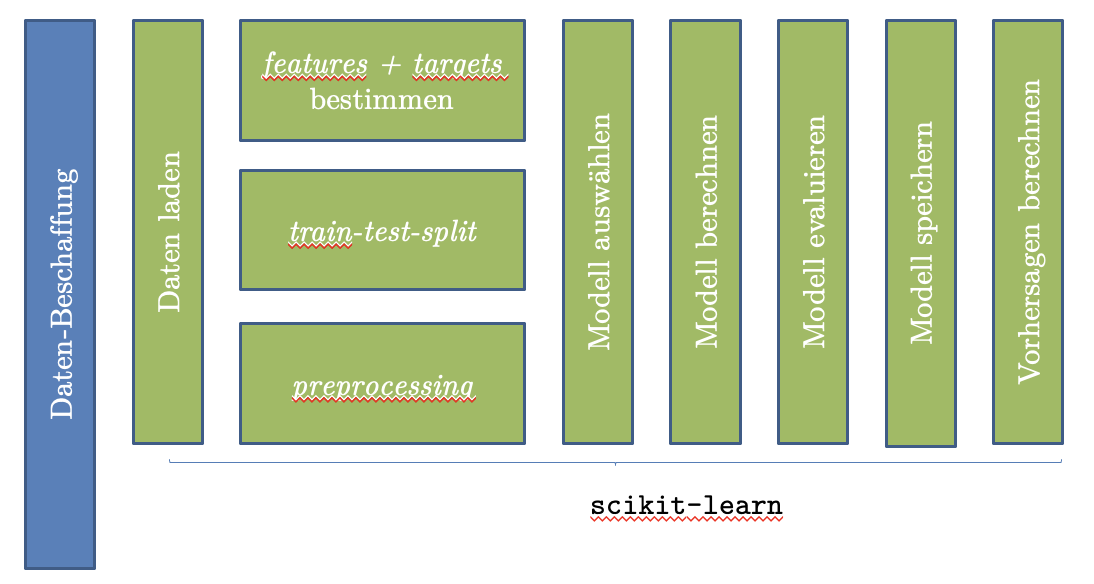
\includegraphics[width=0.9\linewidth]{pipeline.png}
\end{center}

Die obige Abbildung zeigt den typischen Arbeitsablauf bei einem ML-Projekt mit \texttt{scikit-learn}:

\begin{enumerate}
  \item \textbf{Daten-Beschaffung:} Die Daten müssen zunächst aus einer Quelle (z. B. CSV-Datei, Datenbank, API) bezogen werden. Dabei kann Ihnen \texttt{scikit-learn} für gewöhnlich nicht helfen, ausser Sie greifen auf einer der mitgelieferten Datensätzen zur Demonstration zurück (wie wir es gleich tun werden).
  \item \textbf{Daten laden:} Anschliessend werden die Daten in \texttt{python} eingelesen.
  \item \textbf{\textit{features} und \textit{targets} bestimmen:} Es wird festgelegt, welcher Teil der Daten als Eingabe (features, meist \texttt{X}) und welche als Zielvariable (target, meist \texttt{y}) verwendet werden.
  \item \textbf{\textit{train-test-split}:} Der Datensatz wird aufgeteilt in Trainings- und Testdaten, um eine faire Evaluierung zu ermöglichen.
  \item \textbf{\textit{preprocessing}:} Die Daten werden vorbereitet (z. B. skaliert), um für die Algorithmen geeignet zu sein.
  \item \textbf{Modell auswählen:} Es wird ein passender Algorithmus gewählt (z. B. Entscheidungsbaum).
  \item \textbf{Modell berechnen:} Das Modell wird mit den Trainingsdaten trainiert (Methode: \texttt{.fit()}).
  \item \textbf{Modell evaluieren:} Das Modell wird mit den Testdaten getestet, z. B. über \texttt{.score()} oder \texttt{confusion\_matrix()}.
  \item \textbf{Modell speichern:} Gute Modelle können gespeichert werden, z. B. mit \texttt{joblib.dump()}.
  \item \textbf{Vorhersagen berechnen:} Für neue, unbekannte Daten können Vorhersagen getroffen werden (\texttt{.predict()}).
\end{enumerate}

Wir gehen nun auf die einzelnen Schritte genauer ein!

\begin{hinweis}
    Da wir uns nun in die Welt von Python begeben, ist es vielleicht einfacher, wenn Sie dieser LPU mit dem beiliegenden Notizbuch \texttt{files/LA\_1650} folgen. Dort können Sie die Befehle, welche in diesem Kapitel aufgelistet sind, direkt ausprobieren.
\end{hinweis}

Bevor Sie überhaupt etwas mit \texttt{scikit-learn} tun können, müssen Sie es zunächst installieren. Dafür verwenden Sie in Ihrem Terminal folgenden Befehl:

\begin{lstlisting}[language=Bash]
pip install sklearn
\end{lstlisting}

Falls Sie im Notizbuch sind, können Sie dort einfach die Zelle \texttt{!pip install sklearn} ausführen.


\subsubsection*{Iris-Datensatz}
Ein typischer Einstieg in die ML-Welt erfolgt mit dem berühmten Iris-Datensatz, bei dem für verschiedene Iris-Blumenarten L"angen von Bl"uten- und Kelchbl"attern gemessen wurden. Ziel ist es, anhand dieser Merkmale (\textit{features}) die Blumenart (\textit{target}) vorherzusagen. Dieses Beispiel gilt als das \texttt{Hello World} in der Welt des maschinellen Lernens!

\begin{center}
  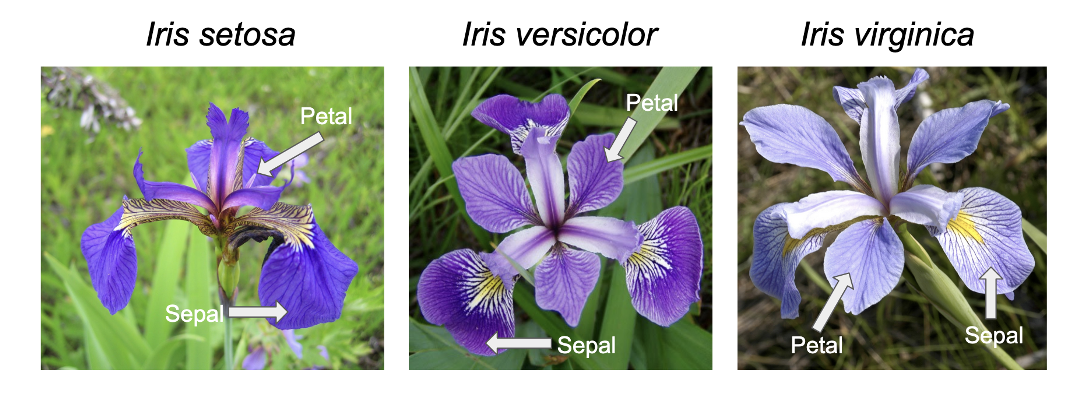
\includegraphics[width=0.9\linewidth]{iris.png}
\end{center}

Um diesen Datensatz einfach zu importieren, verwenden Sie folgenden Befehl:

\begin{lstlisting}[language=Python]
from sklearn.datasets import load_iris
iris = load_iris(as_frame=True)
\end{lstlisting}

Der Parameter \texttt{as\_frame} erlaubt uns, den Datensatz als \texttt{pandas DataFrame}-Objekt zu laden. Der Umgang mit solchen Objekten ist — wie Sie gleich sehen werden — sehr intuitiv und erlaubt es Ihnen, die Daten wie eine Tabelle zu behandeln.

\subsubsection*{\textit{target} und \textit{features}}
In diesem Schritt entscheiden Sie, was genau Sie vorhersagen möchten (das nennt man \textit{target} oder auch \textit{Zielvariable}), und welche Daten dafür als Grundlage dienen sollen (das sind die \textit{features}). Das variiert je nach Datensatz und Ihrem Interesse. Mit demselben Datensatz können Sie ganz unterschiedliche Modelle produzieren, je nachdem, wie Sie das \textit{target} setzen.



\begin{table}[h!]
\centering
\begin{tabular}{|c|c|c|c|c|c|}
\hline
\textbf{age} & \textbf{sex} & \textbf{bmi} & \textbf{smoker} & \textbf{region} & \textbf{health insurance charges} \\
\hline
19 & \male & 27.9  & yes & southwest & 16884 \\
18 & \female & 33.77 & no  & southeast & 1725  \\
28 & \female & 33.0  & no  & southeast & 4449  \\
33 & \female & 22.0  & no  & northwest & 8240  \\
\hline
\end{tabular}
\caption{Beispieldatensatz zu Gesundheitskosten und personenbezogenen Merkmalen}
\end{table}

Aus den Daten in der Tabelle oben können Sie bspw. ein Modell erstellen, was die Krankenkasse-Prämie berechnet basierend auf Alter, BMI und Tabakkonsum. In dem Fall wäre die Prämie das \textit{target} (nachfolgend \colorbox{lightgray}{\textcolor{targetred}{rot}}) und Alter, BMI und Tabakkonsum die \textit{features} (nachfolgend \colorbox{lightgray}{\textcolor{featuregreen}{grün}}). 

\begin{table}[h!]
\centering
\rowcolors{2}{white}{gray!10}
\begin{tabular}{|>{\columncolor{featuregreen}}c|
                c|
                >{\columncolor{featuregreen}}c|
                >{\columncolor{featuregreen}}c|
                c|
                >{\columncolor{targetred}}c|}
\hline
\textbf{age} & \textbf{sex} & \textbf{bmi} & \textbf{smoker} & \textbf{region} & \textbf{health insurance charges} \\
\hline
19 & ♀ & 27.9  & yes & southwest & 16884 \\
18 & ♂ & 33.77 & no  & southeast & 1725  \\
28 & ♂ & 33.0  & no  & southeast & 4449  \\
33 & ♂ & 22.0  & no  & northwest & 8240  \\
\hline
\end{tabular}
\caption{Variante 1: Vorhersage der Krankenkassenprämie aus Alter, BMI und Rauchverhalten}
\end{table}



Aber Sie könnten auch versuchen, den BMI vorherzusagen (\textit{target}) ausgehend auf Alter, Wohnort und Geschlecht (\textit{features}).

\begin{table}[h!]
\centering
\rowcolors{2}{white}{gray!10}
\begin{tabular}{|>{\columncolor{featuregreen}}c|
                >{\columncolor{featuregreen}}c|
                >{\columncolor{targetred}}c|
                c|
                >{\columncolor{featuregreen}}c|
                c|}
\hline
\textbf{age} & \textbf{sex} & \textbf{bmi} & \textbf{smoker} & \textbf{region} & \textbf{health insurance charges} \\
\hline
19 & ♀ & 27.9  & yes & southwest & 16884 \\
18 & ♂ & 33.77 & no  & southeast & 1725  \\
28 & ♂ & 33.0  & no  & southeast & 4449  \\
33 & ♂ & 22.0  & no  & northwest & 8240  \\
\hline
\end{tabular}
\caption{Variante 2: Vorhersage des BMI aus Alter, Geschlecht und Region}
\end{table}




Im Falle unseres Iris-Datensatzes wird uns das Leben hier aber sehr einfach gemacht: Im Datensatz sind die Kolonnen bereits mit \texttt{.data} und \texttt{.target} benannt. \texttt{.data} enthält die Längen der Blüten, und \texttt{.target} die Kategorisierung (\texttt{0} für \textit{Iris setosa}, \texttt{1} für \textit{Iris versicolor} und \texttt{2} für \textit{Iris virginica}). Wir müssen also diese Kolonnen lediglich in unterschiedlichen Variablen speichern, um diese Unterteilung in \textit{target} und \textit{features} zu machen:

\begin{lstlisting}[language=Python]
X = iris.data
y = iris.target
\end{lstlisting}

Wir hätten \texttt{X} und \texttt{y} auch \texttt{features} und \texttt{target} nennen können; aber diese Nomenklatur hat sich für ML-Code eingebürgert. Im Notizbuch können Sie sich mit \texttt{X[:10], y[:10]} auch anzeigen lassen, was nun in diesen Variablen gespeichert wurde.

\begin{theorie}
    Im maschinellen Lernen bezeichnet \textit{target} die \textit{Zielvariable}, also das, was ein Modell vorhersagen können soll. Im Code wird diese üblicherweise mit \texttt{y} bezeichnet.

    \textit{features} nennen wir die Daten, die wir zur Berechnung des \textit{target}s heranziehen. Als Variable im Code heissen diese \texttt{X}.
\end{theorie}

\subsubsection*{\textit{train-test split}}

Wenn ein Modell trainiert wird, besteht die Gefahr, dass es die vorhandenen Daten zu gut lernt – man spricht dann von einer ``Überanpassung'' (\textit{overfitting}). Ein solches Modell funktioniert zwar sehr gut auf den Daten, die es bereits kennt, aber schlecht auf neuen, unbekannten Daten. Das ist ein bisschen wie ``auswendig lernen, ohne zu verstehen''.

\begin{aufgabe}{1: \textit{overfitting} oder echtes Verständnis?}

Stellen Sie sich vor, Ihre Sitznachbarin möchte unbedingt eine gute Note in der nächsten Biologieprüfung. Sie weiss, dass die Lehrperson letztes Jahr eine Prüfung mit 20 Fragen gestellt hat – und dass der genaue Wortlaut dieser alten Prüfung noch im Umlauf ist.

Sie entscheidet sich, diese alte Prüfung auswendig zu lernen – inklusive der genauen Fragestellung und aller Antworten. Am Prüfungstag stellt sich jedoch heraus: Die Lehrperson hat die Fragen leicht verändert.

Hat Ihre Sitznachbarin ``gelernt'' oder nur ``auswendig gelernt''? Was wird das Prüfungsergebnis vermutlich zeigen? Und was hat das mit maschinellem Lernen zu tun?

\begin{itemize}
  \item Erklären Sie den Begriff \textit{overfitting} mit eigenen Worten anhand dieses Beispiels.
  \item Überlegen Sie, wie man das beim Trainieren eines ML-Modells vermeiden könnte.
\end{itemize}
\end{aufgabe}

Analog müssen wir also auch bei unseren Modellen mit Daten, die das Modell noch nicht gesehen hat, aber für die wir als ``Lehrer'' die korrekte Antwort kennen, die Qualität unseres Modells testen, bevor wir es in die freie Wildbahn entlassen.

Aus diesem Grund werden unsere Daten eingeteilt in einen \textit{train} und einen \textit{test}-Teil. Die \textit{train}-Daten (wie \textit{training}, nicht wie das Verkehrsmittel) dienen als Grundlage, um ein Modell zu berechnen; und die Test-Daten werden verwendet, um zu überprüfen, wie gut das Modell für Daten ist, die es noch nicht kennt.

Der \textit{train}- und \textit{test}-Teil sind beide jeweils wie vorhin unterteilt in \texttt{X} und \texttt{y}, wie die nachfolgende Abbildung veranschaulicht:

\vspace{1em}
\begin{center}
  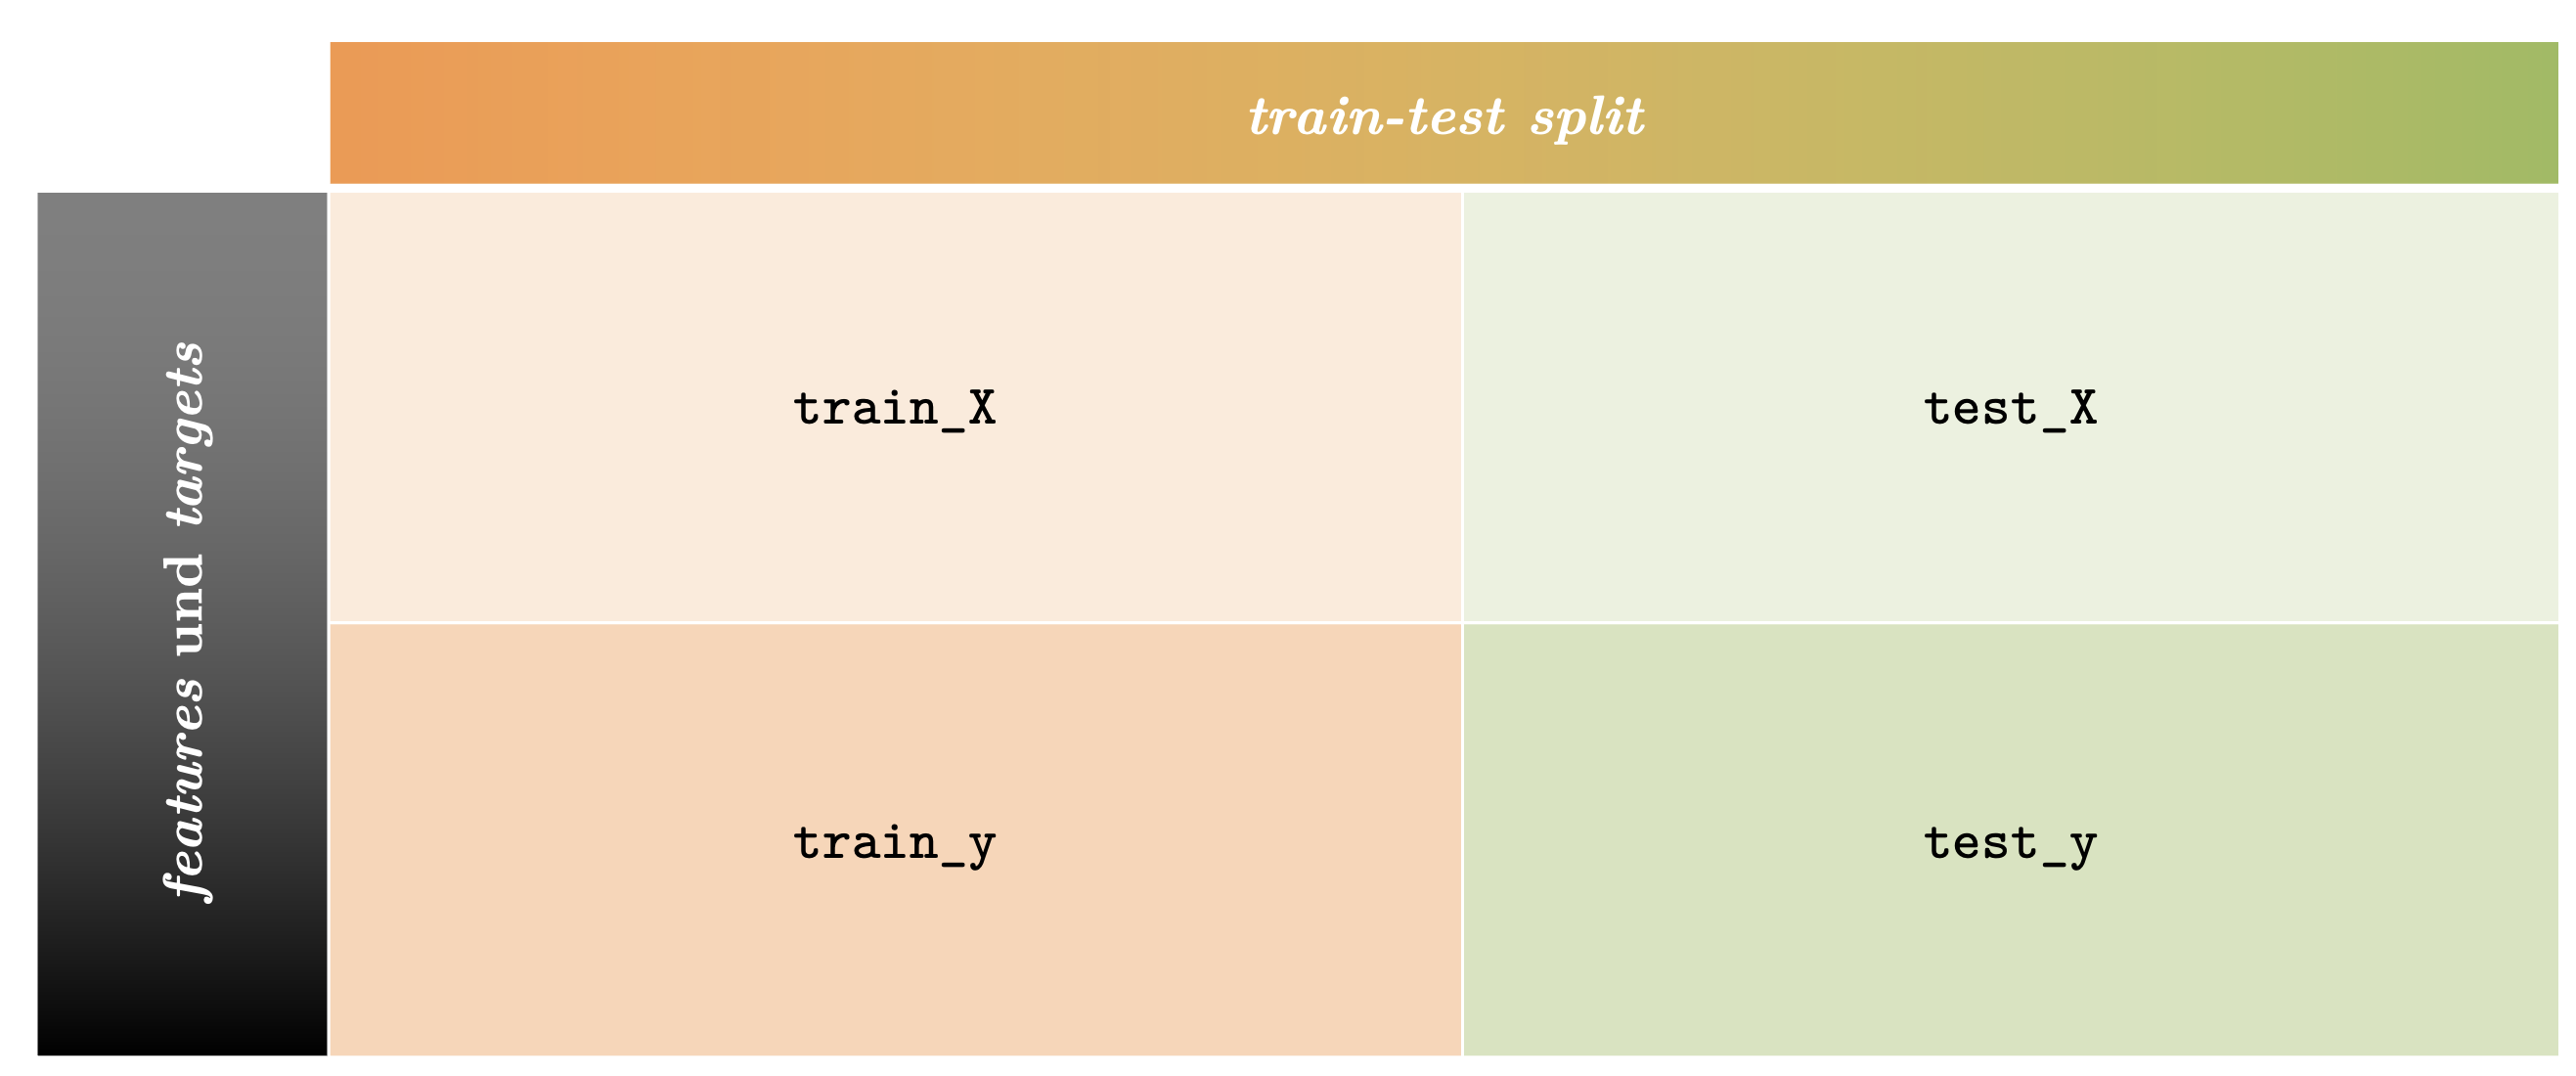
\includegraphics[width=0.9\linewidth]{testtrain.png}
\end{center}

Die meisten fortgeschrittenen Algorithmen werden \textit{iterativ}, das heisst, in mehreren Runden, ausgehend von den \textit{train}-Daten berechnet. Der Algorithmus bekommt also die Test-Daten hier nicht zu Gesicht. Nach jeder Runde wird das Modell getestet, indem die Vorhersage des Modells ausgehend von den \texttt{X}-Werten der Test-Daten mit den tatsächlichen \texttt{y}-Werten der Test-Daten verglichen wird. So kann im Vorfeld berechnet werden, wie gut das Modell für neue Daten Vorhersagen treffen wird.




\begin{figure}[h!]
\centering
\begin{subfigure}[t]{0.45\textwidth}
  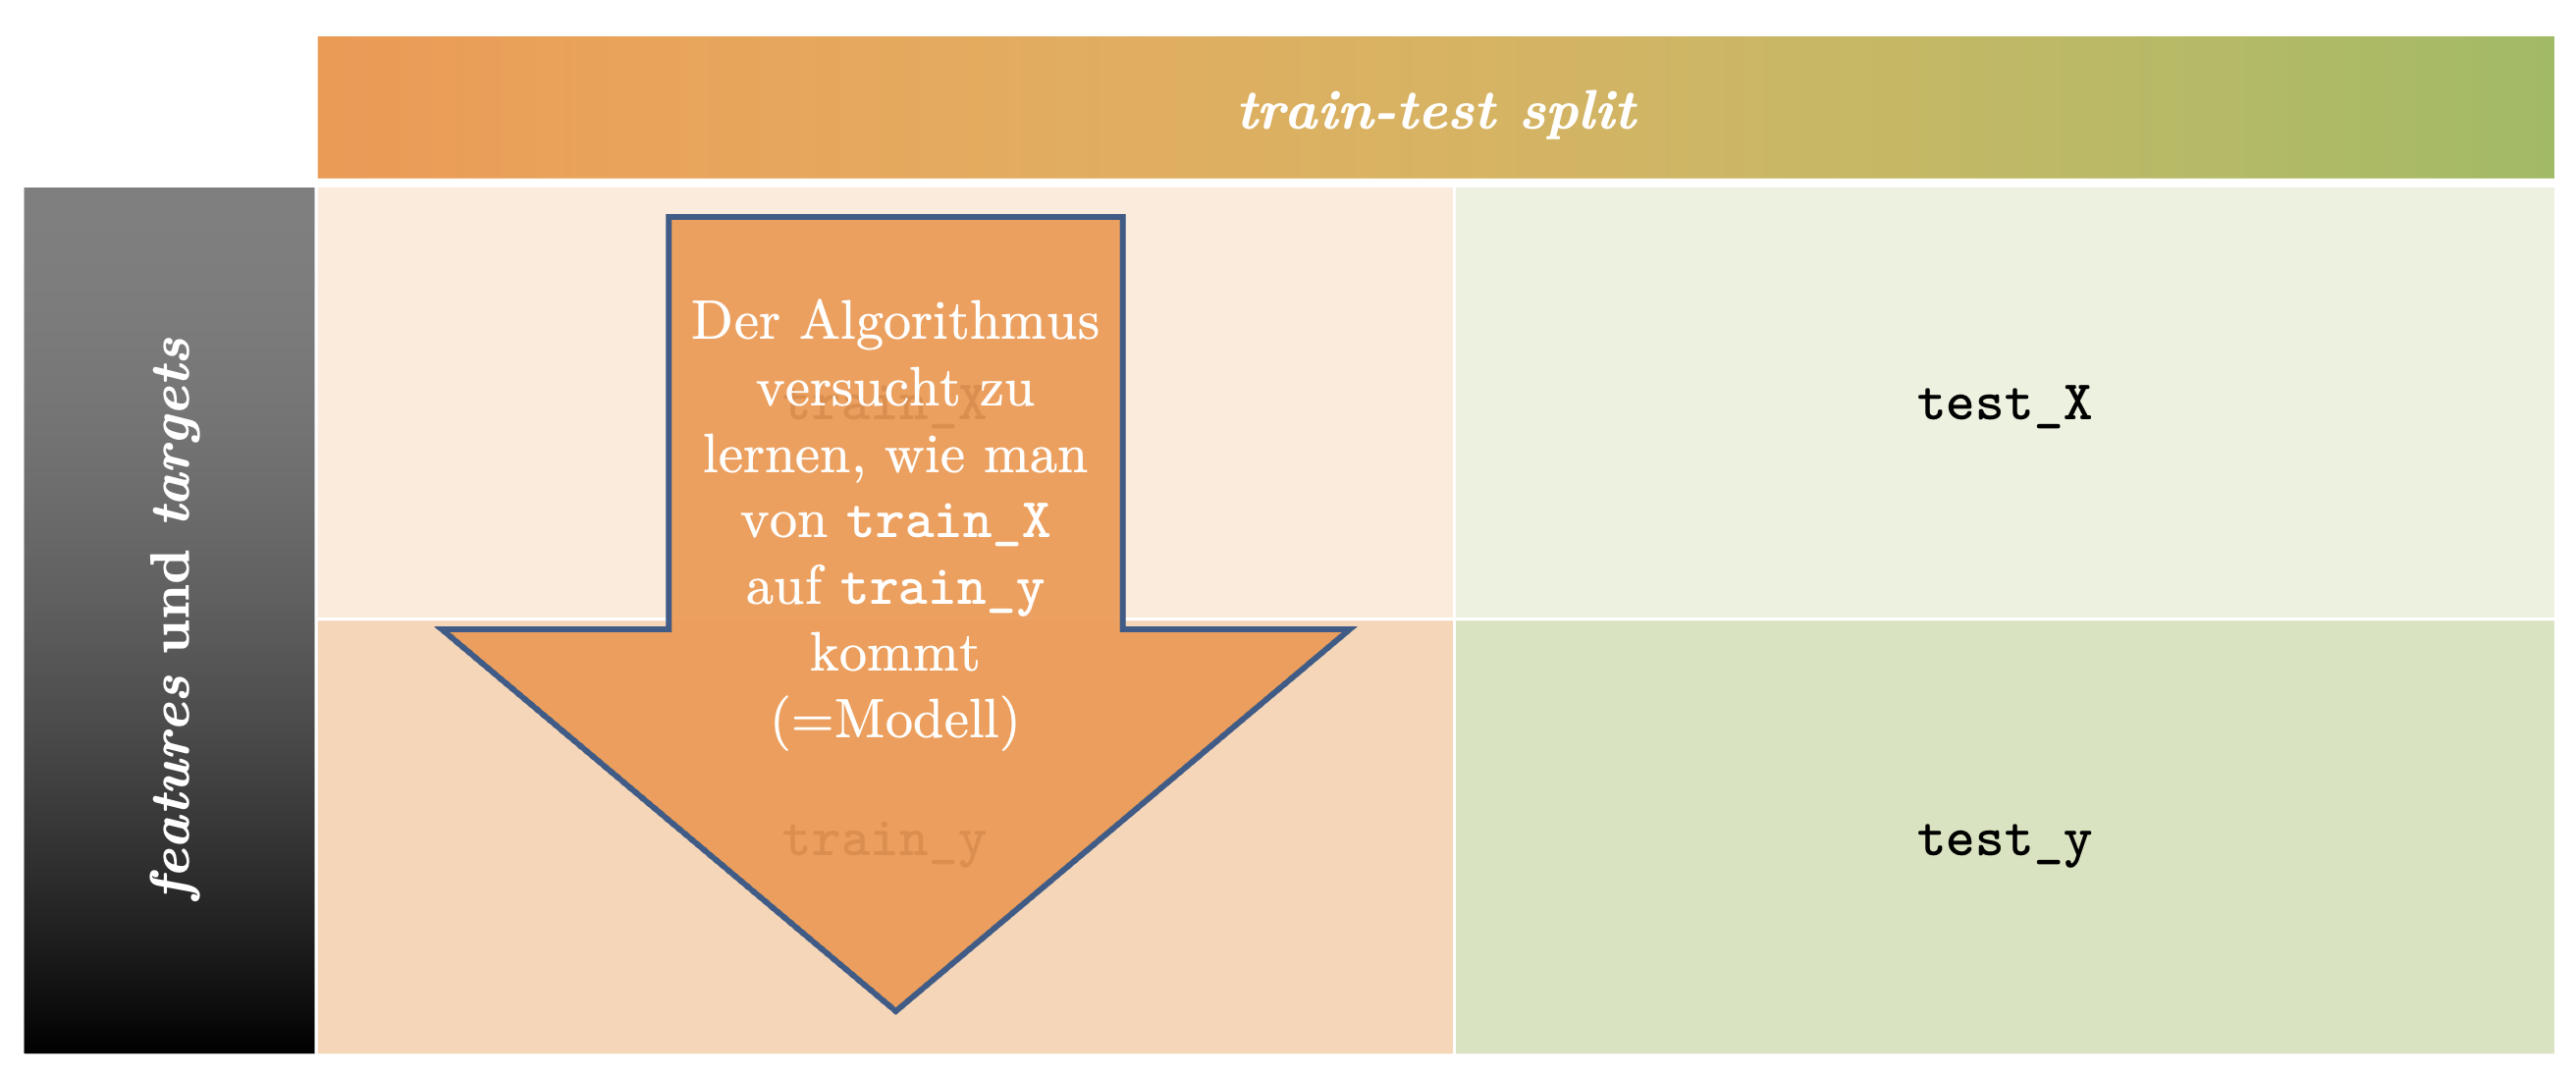
\includegraphics[width=\linewidth, valign=t]{testtrain_1.png}
  \caption{Schritt 1}
\end{subfigure}
\hfill
\begin{subfigure}[t]{0.45\textwidth}
  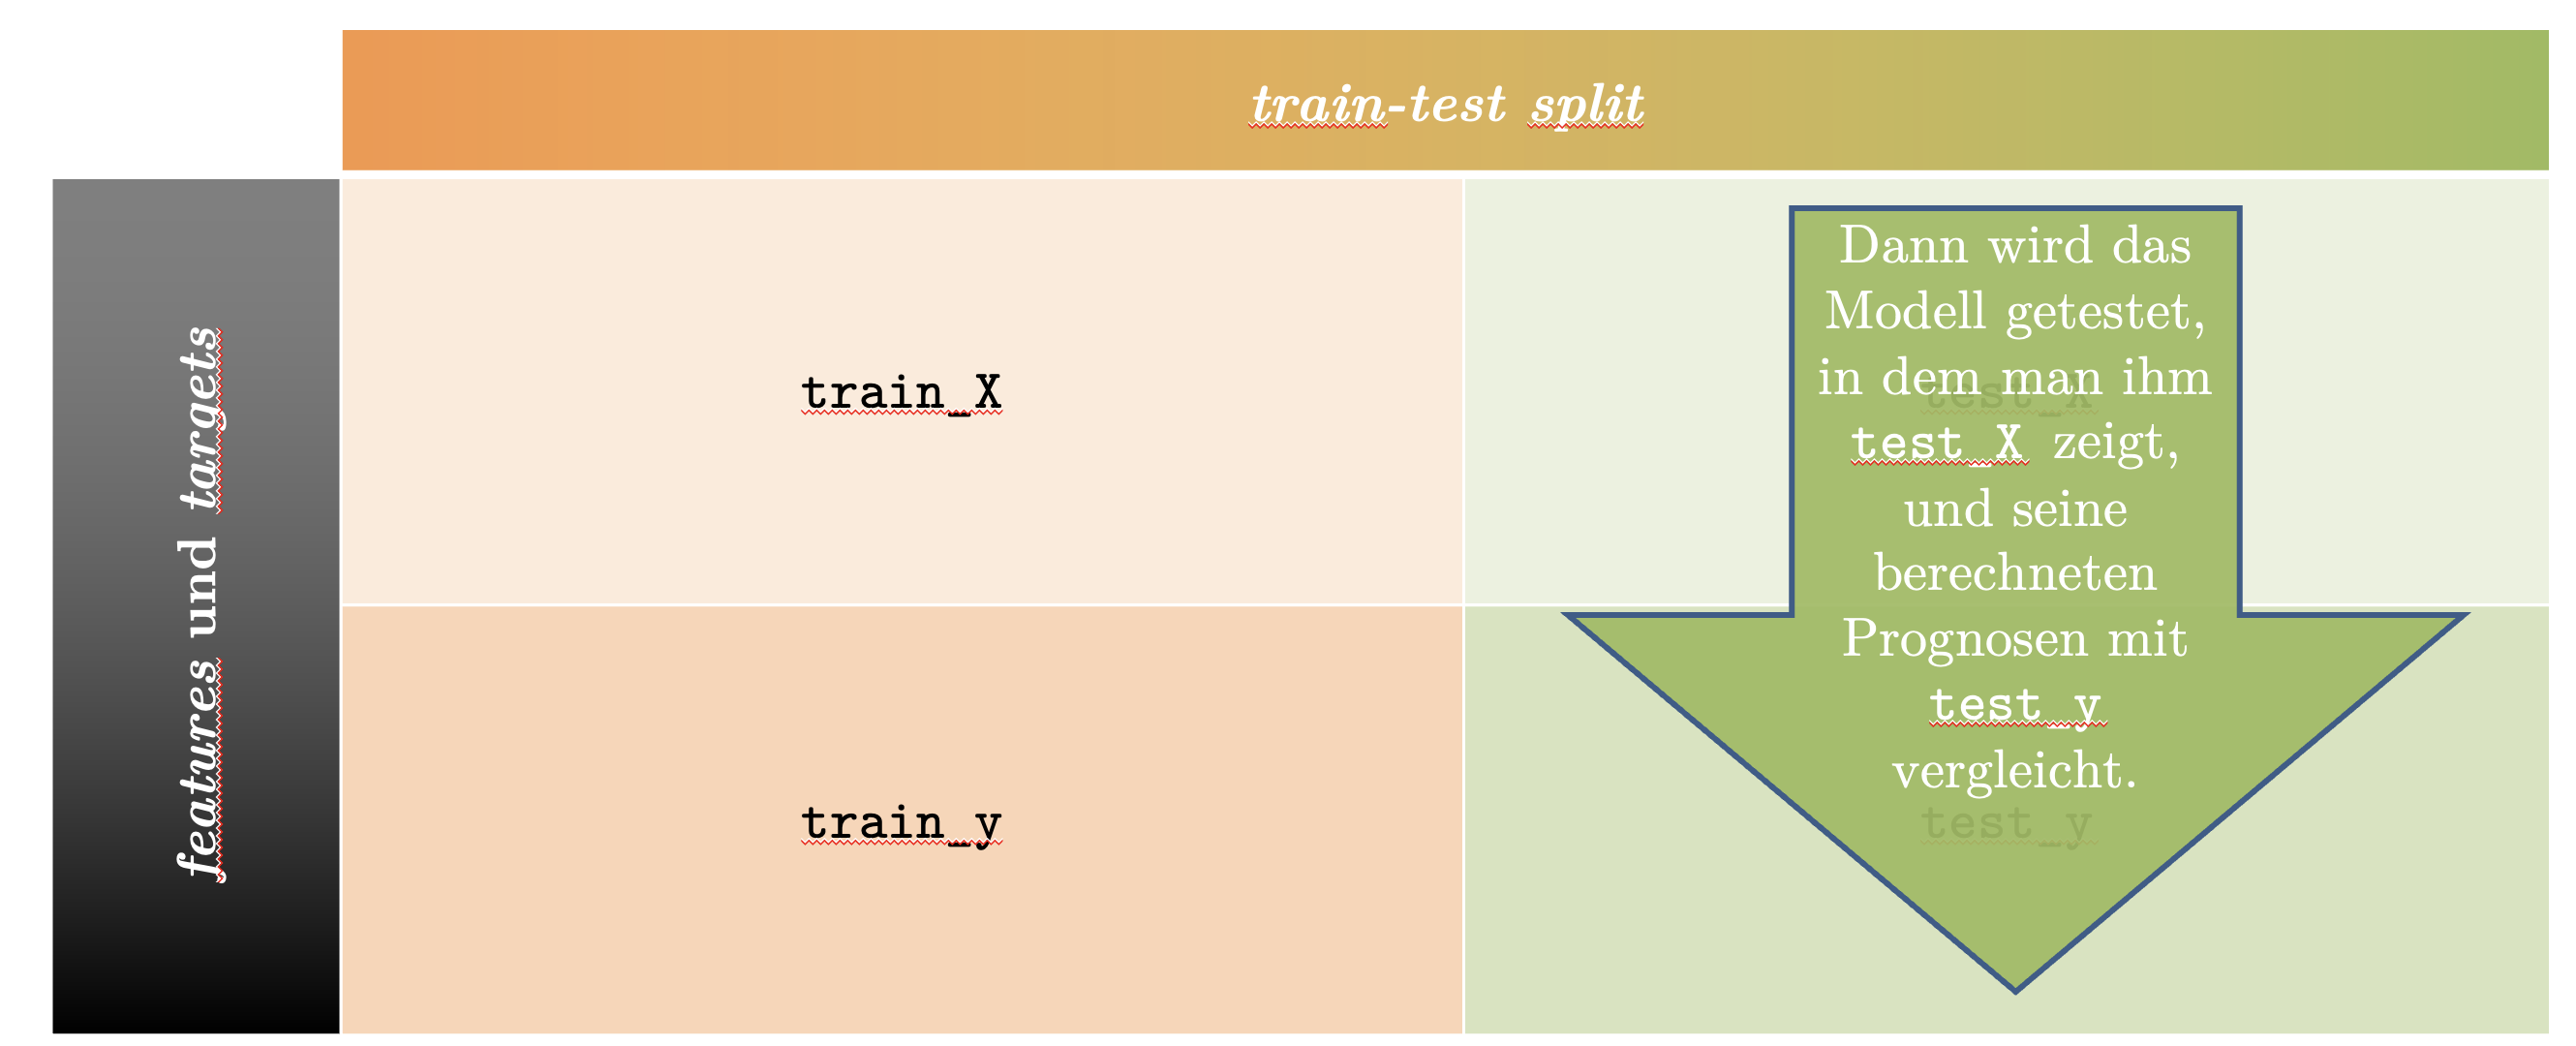
\includegraphics[width=\linewidth, valign=t]{testtrain_2.png}
  \caption{Schritt 2}
\end{subfigure}
\vspace{1em}
\begin{subfigure}[t]{0.45\textwidth}
  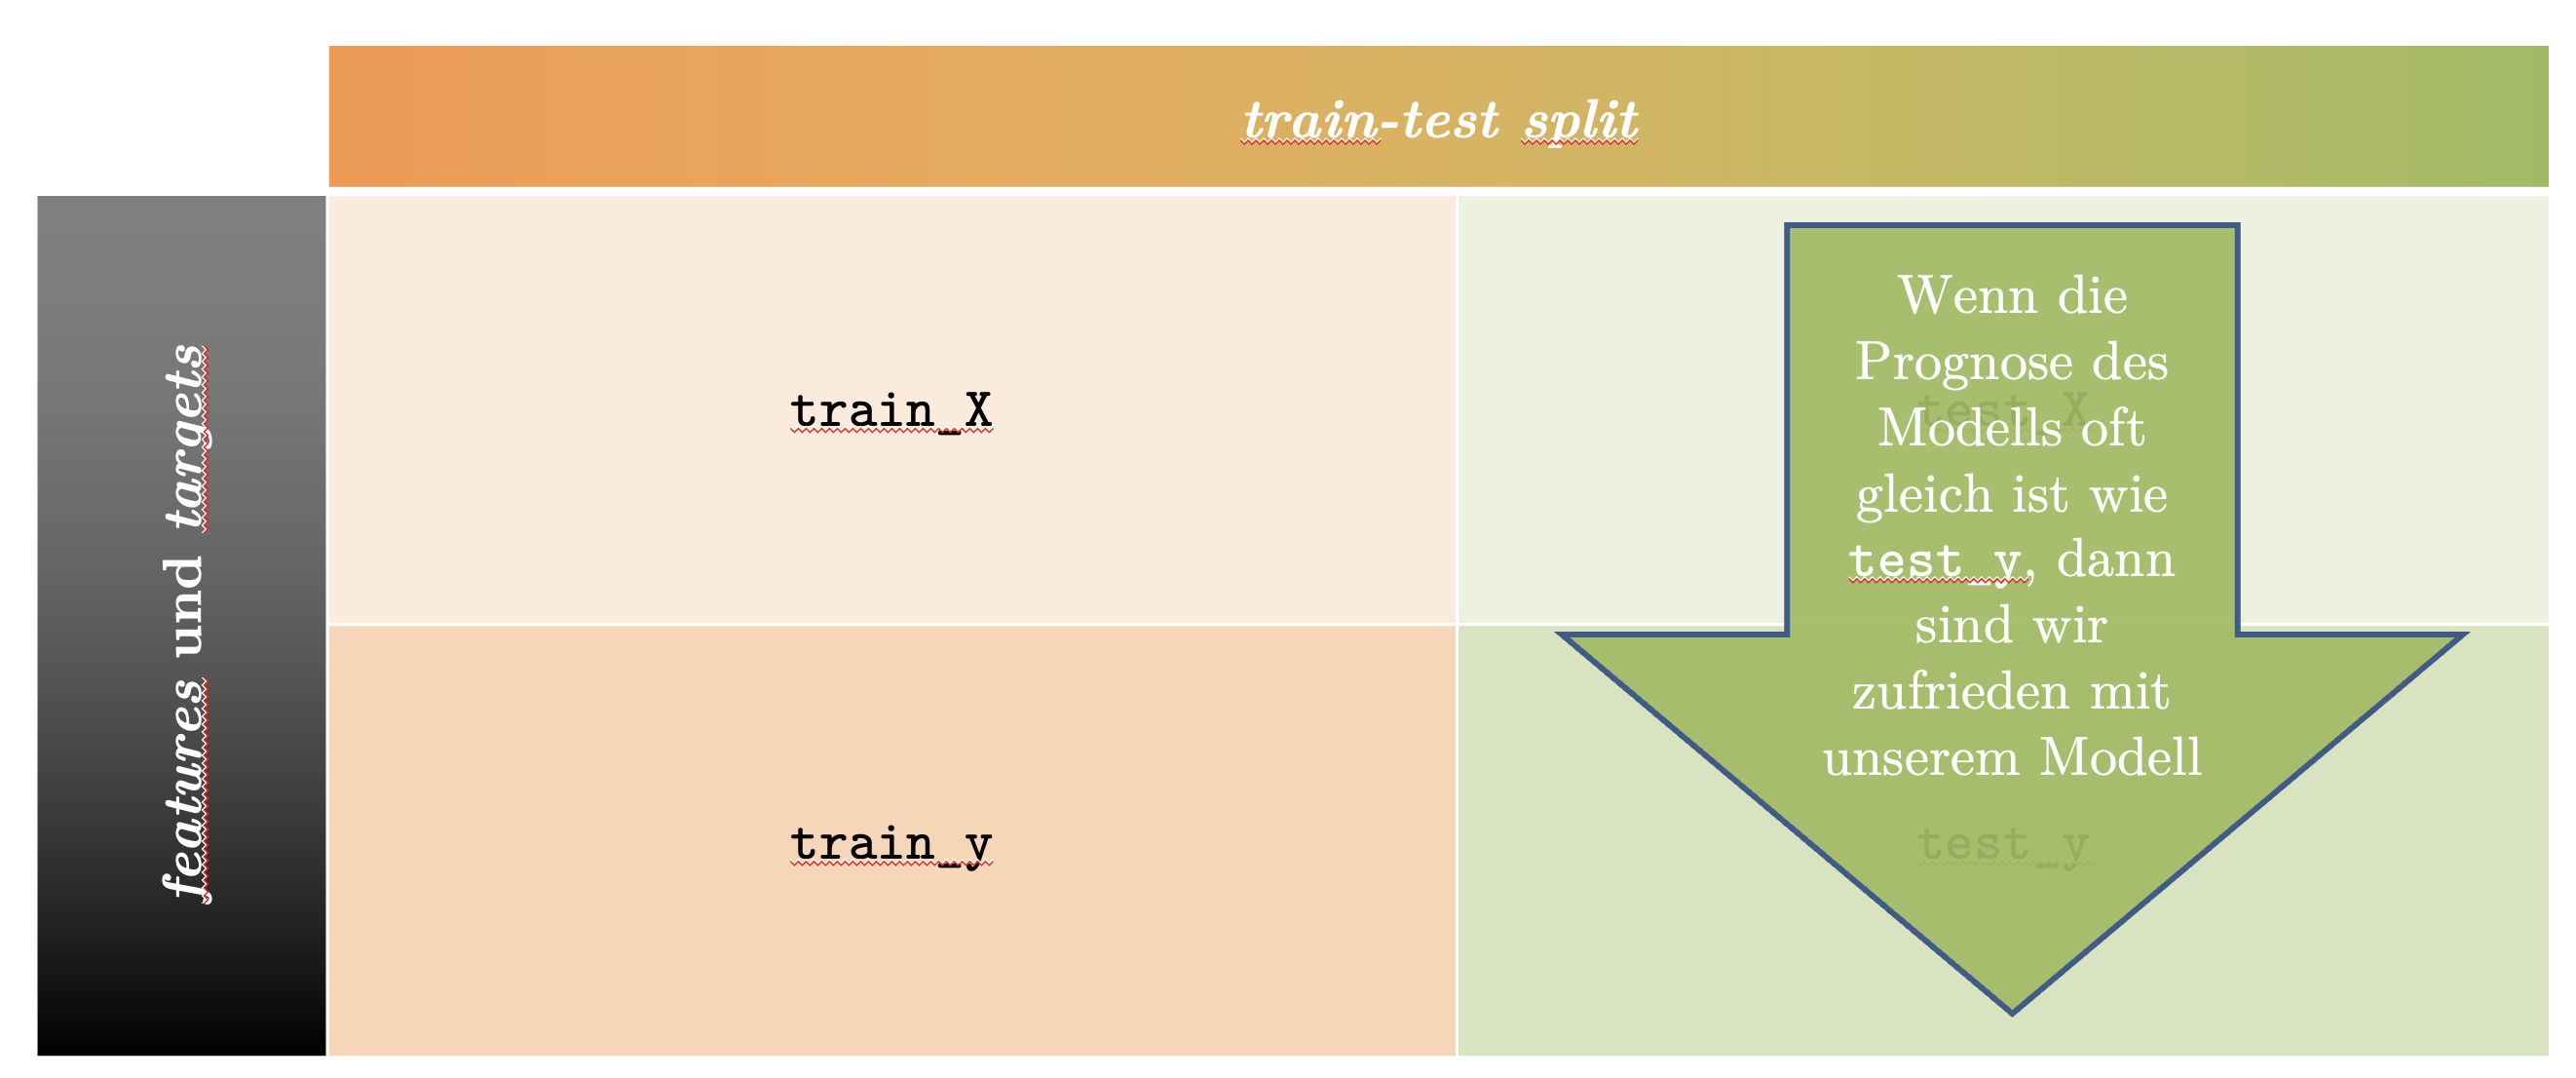
\includegraphics[width=\linewidth, valign=t]{testtrain_3.png}
  \caption{Schritt 3}
\end{subfigure}
\hfill
\begin{subfigure}[t]{0.45\textwidth}
  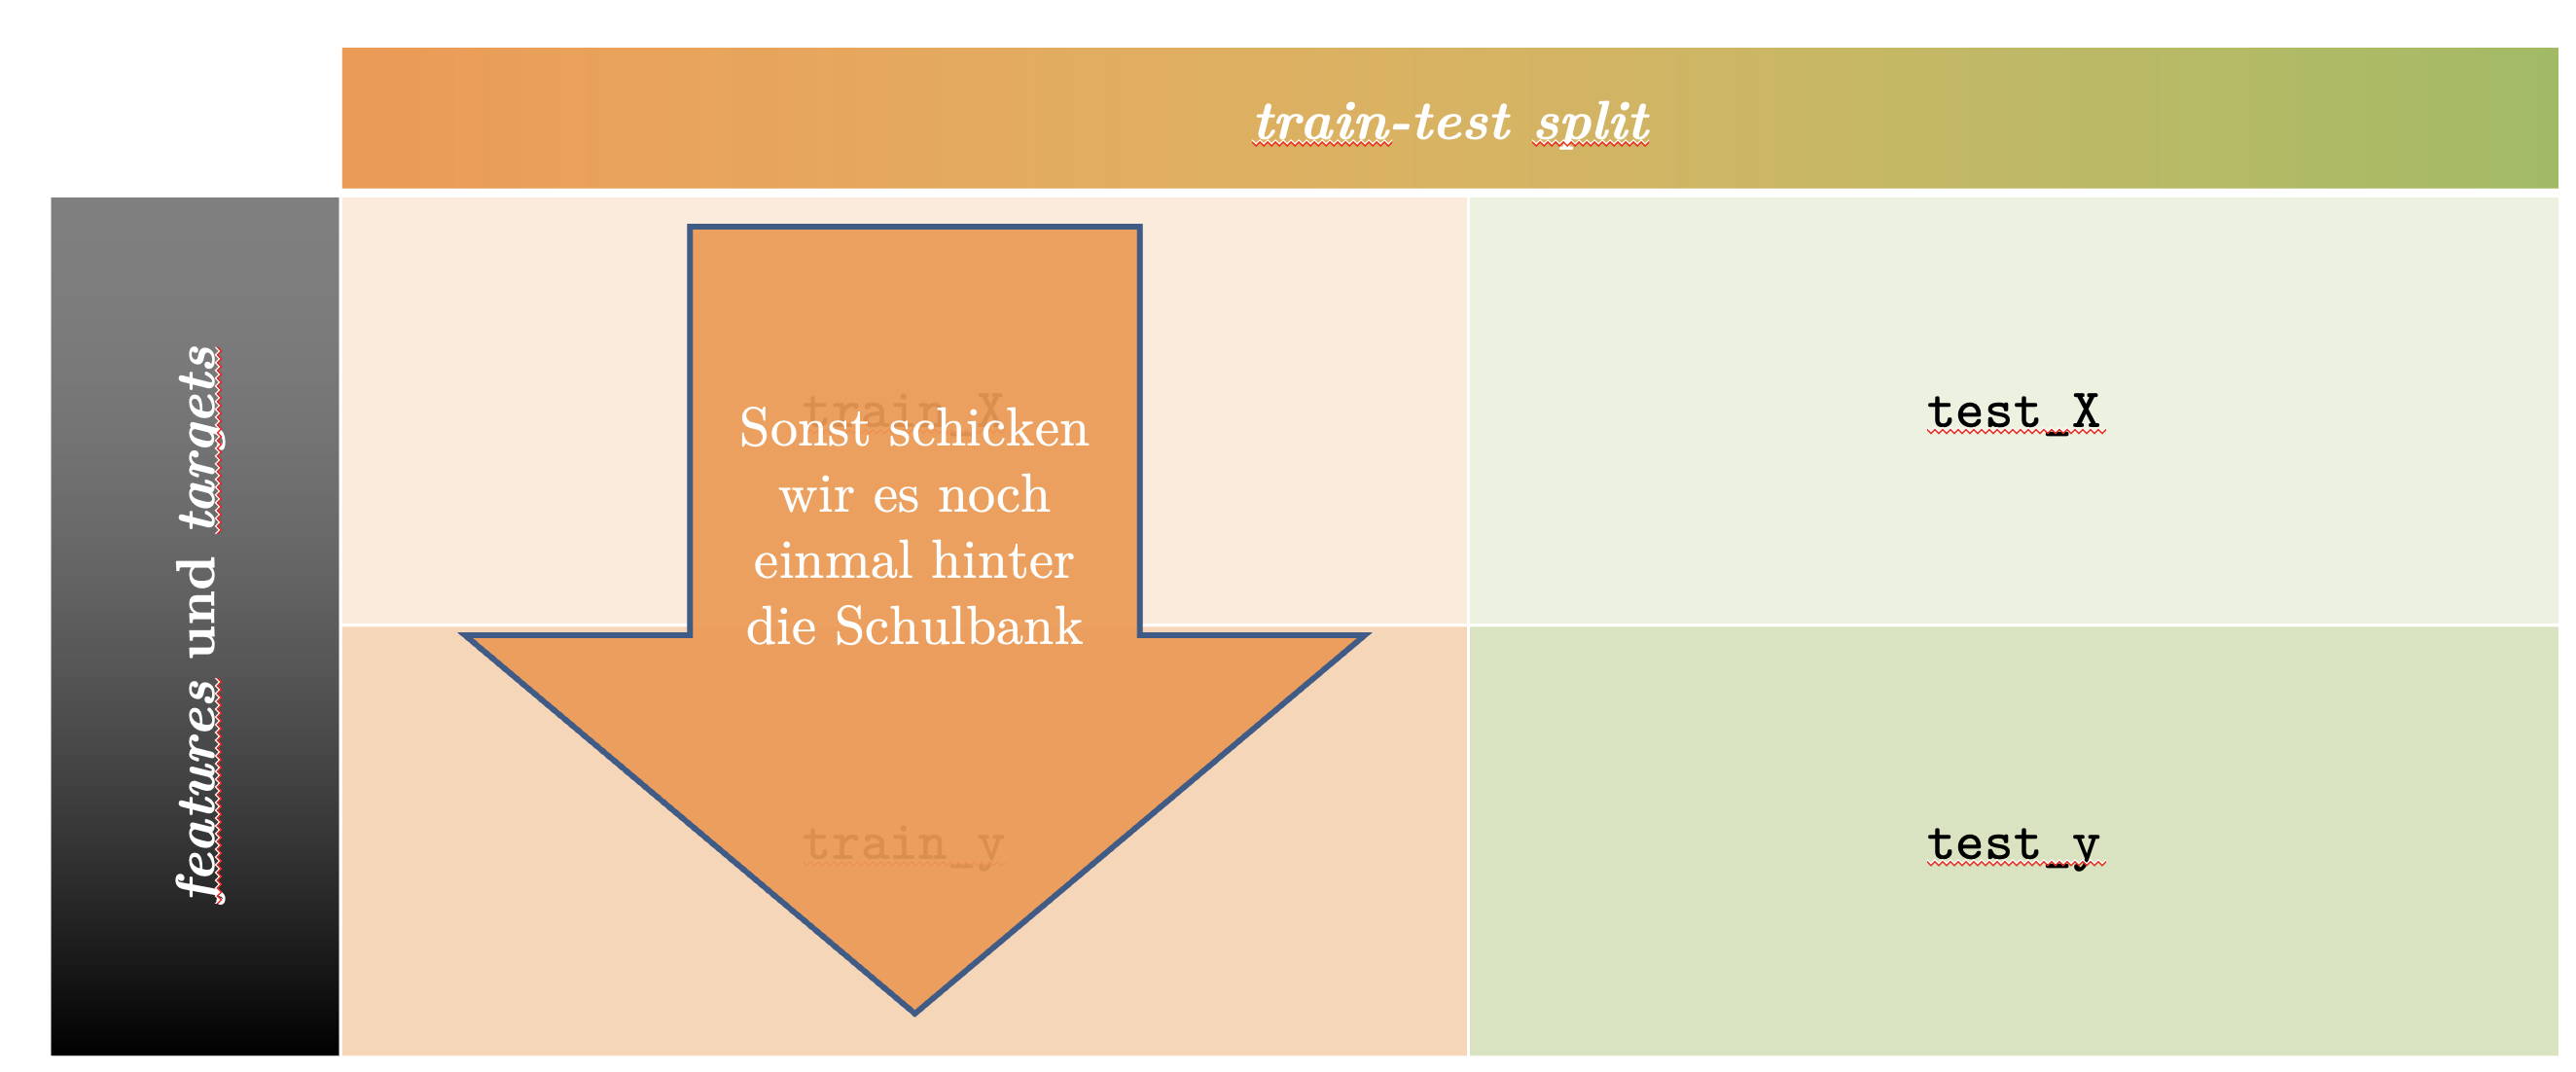
\includegraphics[width=\linewidth, valign=t]{testtrain_4.png}
  \caption{Schritt 4}
\end{subfigure}
\end{figure}






Beim maschinellen Lernen wird der Datensatz in der Regel wie folgt in diese zwei Teile aufgeteilt:
\begin{itemize}
  \item Trainingsdaten: etwa 70–90\,\%
  \item Testdaten: etwa 10–30\,\%
\end{itemize}

Ein Modell benötigt möglichst viele Beispiele, um verlässliche Muster zu erkennen. Wenn zu wenig Daten für das Training verwendet werden, lernt das Modell nicht genug – insbesondere bei kleinen Datensätzen. Ein 50:50-Split ist darum meist ineffizient.

\begin{itemize}
  \item {80\,\% / 20\,\% ist ein verbreiteter Kompromiss: genügend Trainingsdaten, aber auch ausreichend Testdaten für eine seriöse Evaluation.
  \item Bei sehr grossen Datensätzen (z.\,B. >100\,000 Beispiele) sind auch 90\,\% / 10\,\% sinnvoll, da bereits 10\,\% eine grosse Testmenge darstellen.
  \item Bei kleinen Datensätzen wird manchmal eine 70\,\% / 30\,\%-Aufteilung verwendet, um mehr Testbeispiele zu erhalten. (Alternativ kann \textit{cross validation} eingesetzt werden, aber diese sprengt den Rahmen dieser Unterrichtseinheit. Interessierte SuS können \href{https://machinelearningmastery.com/k-fold-cross-validation}{hier}\footnote{\href{https://machinelearningmastery.com/k-fold-cross-validation}{\url{machinelearningmastery.com/k-fold-cross-validation}}} beispielsweise mehr erfahren.)
\end{itemize}

\begin{theorie}

Beim maschinellen Lernen wird der verfügbare Datensatz in zwei Teile aufgeteilt: 
\textbf{Trainingsdaten} (\textit{train set}) und \textbf{Testdaten} (\textit{test set}). Das Modell wird ausschliesslich mit den Trainingsdaten ``gelernt'' – die Testdaten dienen dazu, die Leistung des Modells auf \textit{neuen, unbekannten Daten} zu überprüfen. Nur so kann man feststellen, ob das Modell wirklich generalisiert oder lediglich auswendig gelernt hat (\textit{overfitting}).
\end{theorie}

In \texttt{scikit-learn} ist auch dieser Schritt sehr einfach: Mit dem folgenden Befehl passiert diese Einteilung automatisch:




\begin{lstlisting}[language=Python]
from sklearn.model_selection import train_test_split

X_train, X_test, y_train, y_test = train_test_split(
   X, y, test_size = 0.3, random_state = 42
)
\end{lstlisting}


Die Bedeutung der einzelnen Variablen ist:

\begin{itemize}
  \item \texttt{X}: Variable mit den \textit{features} (z. B. Länge der Blüten, oder Wohnort, Rauchverhalten etc. im Krankenkassen-Beispiel)
  \item \texttt{y}: Variable mit dem \textit{target} (z. B. Iris-Art oder Versicherungskosten)

  \item \texttt{X\_train}: Features der Trainingsdaten
  \item \texttt{X\_test}: Features der Testdaten
  \item \texttt{y\_train}: Zielwerte der Trainingsdaten
  \item \texttt{y\_test}: Zielwerte der Testdaten
\end{itemize}

\texttt{test\_size = 0.3} bedeutet, dass 30\,\% der Daten für das Testset verwendet werden. Da unser Datensatz so klein ist, ist das hier sinnvoll.
\texttt{random\_state = 42} sorgt dafür, dass die Aufteilung \textit{reproduzierbar} ist: Zwar werden die Daten ``zufällig'' in \textit{test}- und \textit{train}-Teile aufgeteilt, aber immer, wenn jemand \texttt{random\_state = 42} für \textit{diesen} Datensatz verwendet, sieht die Aufteilung gleich aus. Würde jemand \texttt{random\_state = 33} verwenden, hingegen, sähe sie anders aus. Das ist wichtig, wenn Sie Ihre Arbeit reproduzierbar machen möchten.

\subsubsection*{Aufbereitung}

Bevor ein ML-Modell mit den Daten trainiert wird, müssen diese oft vorbereitet werden – man spricht von \textit{preprocessing} (wörtlich Vorverarbeitung). Das Ziel ist es, die Daten in eine Form zu bringen, mit der der Algorithmus effizient und korrekt arbeiten kann.

Eine zentrale Technik, die Sie bereits kennen, ist die \textit{Skalierung}. Numerische Werte wie z. B. Alter oder Einkommen werden auf einen gemeinsamen Zahlenbereich gebracht (z. B. $[0,1]$), damit einzelne Spalten das Modell nicht übermässig beeinflussen.

Darüber hinaus gibt es weitere wichtige Möglichkeiten der Aufbereitung:

\begin{itemize}
  \item \textit{one hot encoding:} Kategorische Merkmale wie ``Region'' oder ``Geschlecht'' werden in Zahlen umgewandelt.
  \item Fehlende Werte behandeln: Leere Zellen (NaN) werden z.B. durch Mittelwerte oder spezielle Marker ersetzt.
  \item Text-Vektorisierung: Texte müssen in Zahlen umgewandelt werden, da viele Modelle nicht gut natürlichen Text verarbeiten können. Das wird oft mittels \textit{embeddings} gemacht, sodass der gesamte Text als ein mathematischer Vektor ausgedrückt werden kann. (Dies nur zur Information; diese Technik geht weit über den Rahmen dieser Unterrichtseinheit hinaus.)
\end{itemize}

\texttt{scikit-learn} stellt für all diese Schritte praktische Funktionen bereit, z.B. \texttt{StandardScaler}, \texttt{OneHotEncoder} oder \texttt{SimpleImputer}.

\begin{aufgabe}{2}
Schauen Sie sich den Iris-Datensatz etwas genauer an (bspw. mit \texttt{X[:10], y[:150]} im Notizbuch):

\begin{enumerate}
    \item Finden Sie in diesem Datensatz das oben erwähnte \textit{one hot encoding} wieder?
    \item Die \texttt{X}-Werte enthalten verschiedene Arten von Messungen (nämlich die Breite und Länge der Blütenblätter und die Länge und Breite des Kelchblatts). Befinden sich diese alle im selben Wertebereich? Würden Sie eine Skalierung hier als sinnvoll erachten?
\end{enumerate}
\end{aufgabe}

Wenn wir unsere Daten aufbereiten müssen, dann macht es uns \texttt{scikit-learn} wieder ungemein einfach:
\begin{lstlisting}[language=Python]
from sklearn import preprocessing
scaler = preprocessing.MinMaxScaler()
X_train_scaled = scaler.fit_transform(X_train)
X_test_scaled = scaler.transform(X_test)
\end{lstlisting}

Damit skalieren wir \texttt{X\_train} und \texttt{X\_test} mit dem \texttt{MinMaxScaler}, der alle Werte auf einen Bereich von \texttt{0} bis \texttt{1} bringt. Es gibt auch andere Algorithmen, welche den Wertebereich bspw. auf $[-1,1]$ skalieren. Weiterhin:

\begin{itemize}
  \item \texttt{fit\_transform(X\_train)}: berechnet Minimum und Maximum auf Basis der Trainingsdaten und wendet die Skalierung direkt an.
  \item \texttt{transform(X\_test)}: verwendet genau dieselben minimalen und maximalen Grenzwerte, um auch die Testdaten korrekt zu skalieren.
\end{itemize}

Die Testdaten dürfen nicht in die Berechnung der Skalierung einfliessen, da sonst ein ausgefuchster Algorithmus daraus Rückschlüsse auf die Testdaten schliessen könnte.


\subsubsection*{Modellauswahl}

In \texttt{scikit-learn} stehen viele verschiedene ML-Modelle zur Verfügung. Doch welches Modell ist das Richtige? Natürlich gibt es verschiedene Algorithmen für verschiedene Probleme (bspw. Entscheidungsbäume für Kategorisierung), aber selbst innerhalb einer Problem-Klasse gibt es viele Algorithmen mit unterschiedlichen Vor- und Nachteilen.

In der Praxis testet man oft mehrere Modelle und vergleicht sie anhand ihrer Leistung auf den Test-Daten. \texttt{scikit-learn} macht diesen Vergleich sehr einfach, weil alle Modelle eine ähnliche API (\texttt{fit()}, \texttt{predict()}, \texttt{score()}) verwenden.

Die nachfolgende Grafik gibt aber eine gute Übersicht, was innerhalb von \texttt{sklearn} möglich ist, und wie Sie eine erste Auswahl treffen können:

\begin{center}
  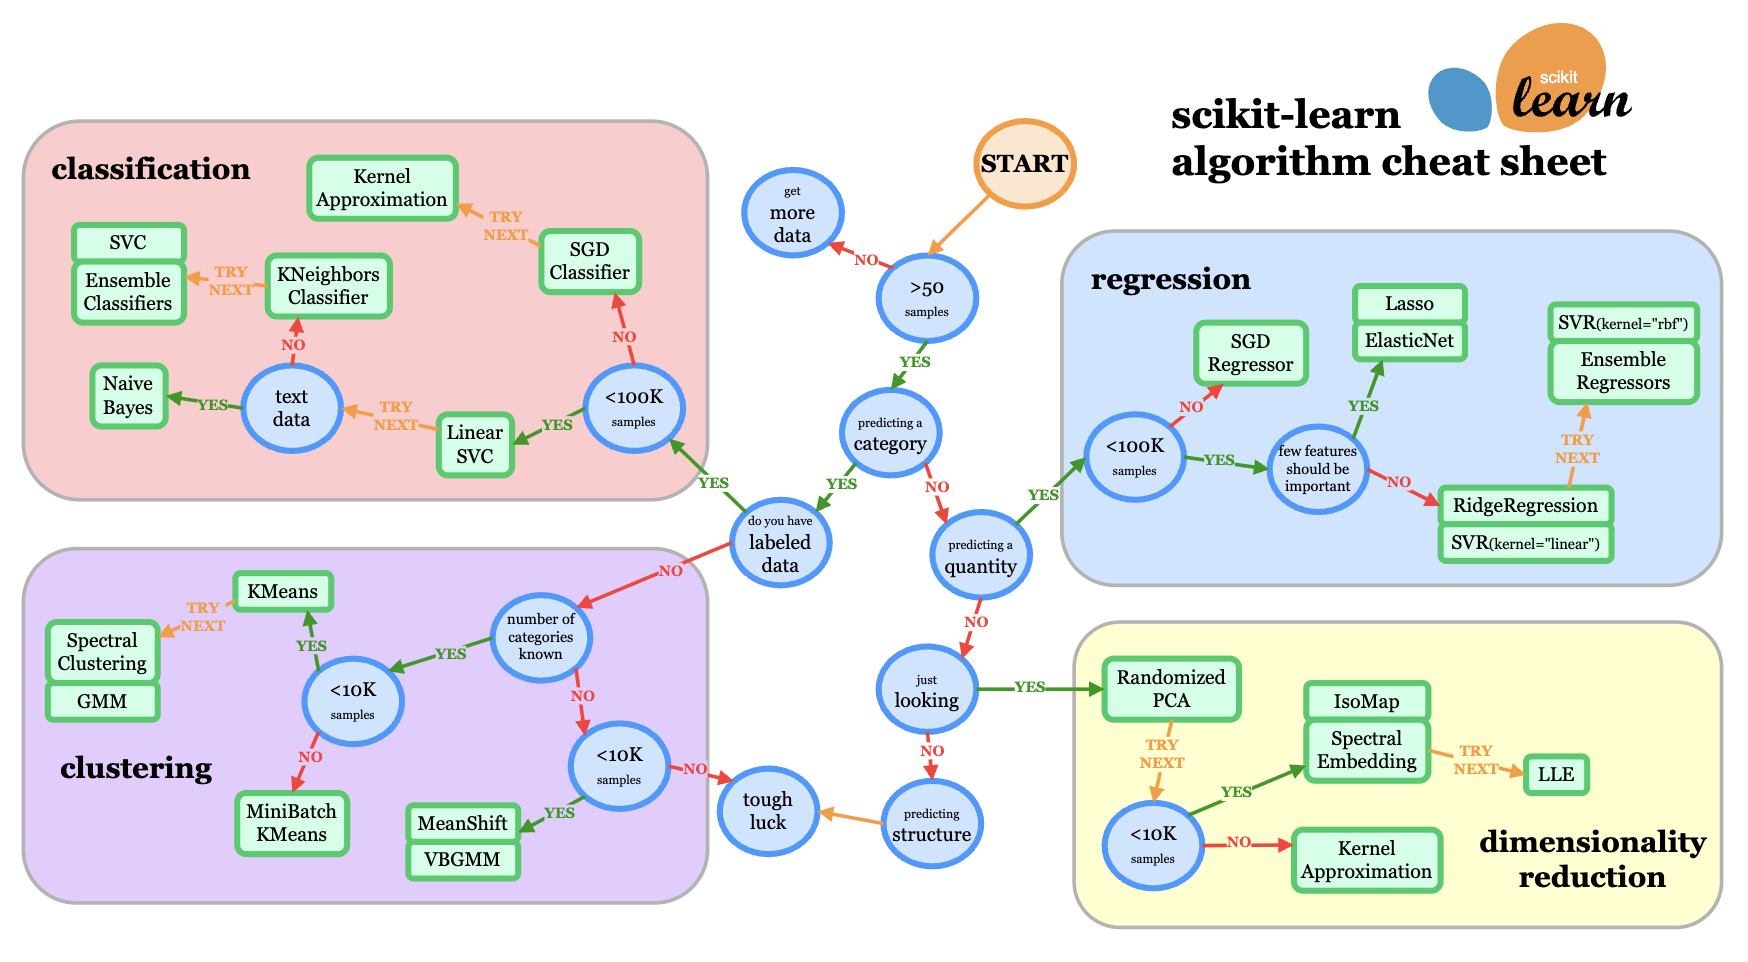
\includegraphics[width=0.9\linewidth]{algos.png}
\end{center}

Für unsere Iris nehmen wir aber einen Algorithmus, den wir bereits kennen: Den Entscheidungsbaum (oder \texttt{DecisionTreeClassifier()} innerhalb von \texttt{sklearn}).


\subsubsection*{Modell berechnen}


Wie eingangs erwähnt ist ein grosser Vorteil von \texttt{scikit learn}, dass verschiedene Algorithmen genau gleich verwendet werden können — obwohl sie sozusagen ``unter der Haube'' ganz anders funktionieren. Die Abstraktion macht den Umgang mit unterschiedlichen Algorithmen sehr angenehm und lädt auch zum Ausprobieren ein! Entscheidend ist hier die \texttt{.fit()}-Funktion, welche unabhängig vom ausgewählten Algorithmus die Berechnung des Modells vornimmt.

Die Funktion \texttt{fit()} ist in \texttt{scikit-learn} der Standardbefehl, um ein Modell zu trainieren. Der Name stammt aus dem Englischen und bedeutet in diesem Zusammenhang so viel wie \textit{anpassen}. Die Idee ist, dass das Modell versucht , möglichst gut zu den Trainingsdaten zu ``passen'' – es sucht ein mathematisches Modell, das den Zusammenhang zwischen den \texttt{features} (\texttt{X\_train}) und dem \texttt{target} (\texttt{y\_train}) beschreibt. Man sagt darum auch: \textit{``Das Modell wird an die Daten angepasst.''}

Im nachfolgenden Beispiel werden ein Entscheidungsbaum und ein KNN (ein Algorithmus, dessen Funktionsweise wir nicht behandelt haben) berechnet - beobachten Sie, wie klein der Unterschied hier ist!

\begin{lstlisting}[language=Python]
from scikit-learn import tree
classifier = tree.DecisionTreeClassifier() 
DT = classifier.fit(X_train,y_train)

from scikit-learn.neighbors import KNeighborsClassifier
classifier = KNeighborsClassifier(n_neighbors = 3) 
KNN = classifier.fit(X_train, y_train)
\end{lstlisting}

Wie Sie im Notizbuch sehen können, erlaubt Ihnen \texttt{sklearn} sogar, den automatisch berechneten Entscheidungsbaum darzustellen!

\subsection*{Evaluieren}
Wir können nun unser Modell \texttt{DT} (oder auch \texttt{KNN}) verwenden, um Vorhersagen zu treffen. Zunächst, bevor wir uns komplett neuen Irissen zuwenden, testen wir aber unser Modell anhand der Testdaten. Sollte sich herausstellen, dass unser Modell schon bei diesen Daten versagt, können wir nochmal über die Bücher. Wichtig ist zu verstehen, dass bei den Testdaten \textit{wir} wissen, was das Resultat sein soll, aber das Modell nicht. Das erlaubt uns überhaupt, zu überprüfen, ob das Modell richtig liegt oder nicht.

Hier ist das Iris-Beispiel sehr illustrativ: Wenn wir direkt, ohne diesen Evaluationsschritt ins Feld gehen, dann müssen wir — ausser Sie hätten eine entsprechende botanische Vorbildung — unserem Modell wohl oder übel glauben, da wir selbst nicht wissen, zu welcher Gattung eine bestimmte Iris gehört.

Die genauen Werte, die wir bei der Evaluation berechnen, sind ein Kapitel für sich; aber um eine Intuition zu bekommen, ob unser Modell eher gut oder schlecht ist, können wir Folgendes tun: Wir verwenden die Testdaten und vergleichen die Vorhersagen des Modells mit den tatsächlichen Werten (\texttt{y\_test}):

\begin{lstlisting}[language=Python]
y_pred = DT.predict(X_test)
\end{lstlisting}

Das Modell berechnet Vorhersagen (\texttt{y\_pred}) basierend auf den Test-\textit{features} \texttt{X\_test}. Diese vergleichen wir mit den echten Zielwerten \texttt{y\_test}.

Für eine erste Einschätzung genügt oft:

\begin{lstlisting}[language=Python]
DT.score(X_test, y_test)
\end{lstlisting}

Dieser Befehl gibt die \textbf{Genauigkeit} (\textit{accuracy}) zurück: den Anteil der Testbeispiele, bei denen das Modell die Klasse korrekt vorhergesagt hat.

Im Notizbuch wird dieser Schritt ganz am Ende durchgeführt, um es spannend zu machen. Dort sieht der Code etwas anders aus: Er zeigt für jede einzelne Zeile in \texttt{X\_test} was der entsprechende, richtige Wert in \texttt{y\_test} ist, und was das Modell vorhersagt.


\subsubsection*{Persistieren}
Auf diesem kleinen Datensatz geht das Berechnen ziemlich schnell voran — in der Wirklichkeit dauert aber das Berechnen eines Modells lange Zeit und nimmt viel Rechenleistung in Anspruch. Darum möchten wir die getane Arbeit auf keinen Fall wegwerfen und speichern (oder in Informatik-Sprache: \textit{persistieren}) unser Modell:

\begin{lstlisting}[language=Python]
import joblib
joblib.dump(DT, 'iris_tree.joblib')
\end{lstlisting}

Hierbei ist \texttt{DT} der Name unseres Modells, also das, was die \texttt{.fit()}-Funktion uns zurückgegeben hat. Mit dem folgenden Code können Sie das Modell später wieder laden - vorausgesetzt, dass Sie die Datei \texttt{iris\_tree.joblib} noch haben.

\begin{lstlisting}[language=Python]
DT = joblib.load('iris_tree.joblib')
\end{lstlisting}

\subsubsection*{Vorhersagen}
Nun sind wir endlich bereit, und wagen uns hinaus in die Natur mit unserem Modell. Wir stellen uns vor, dass wir als Belohnung für unsere Mühe zum berühmten Irisgarten des Meiji-Schreines in Tōkyō reisen, in welchem im Juni über 150 verschiedene Irisse blühen! 

\begin{figure}
\begin{center}
  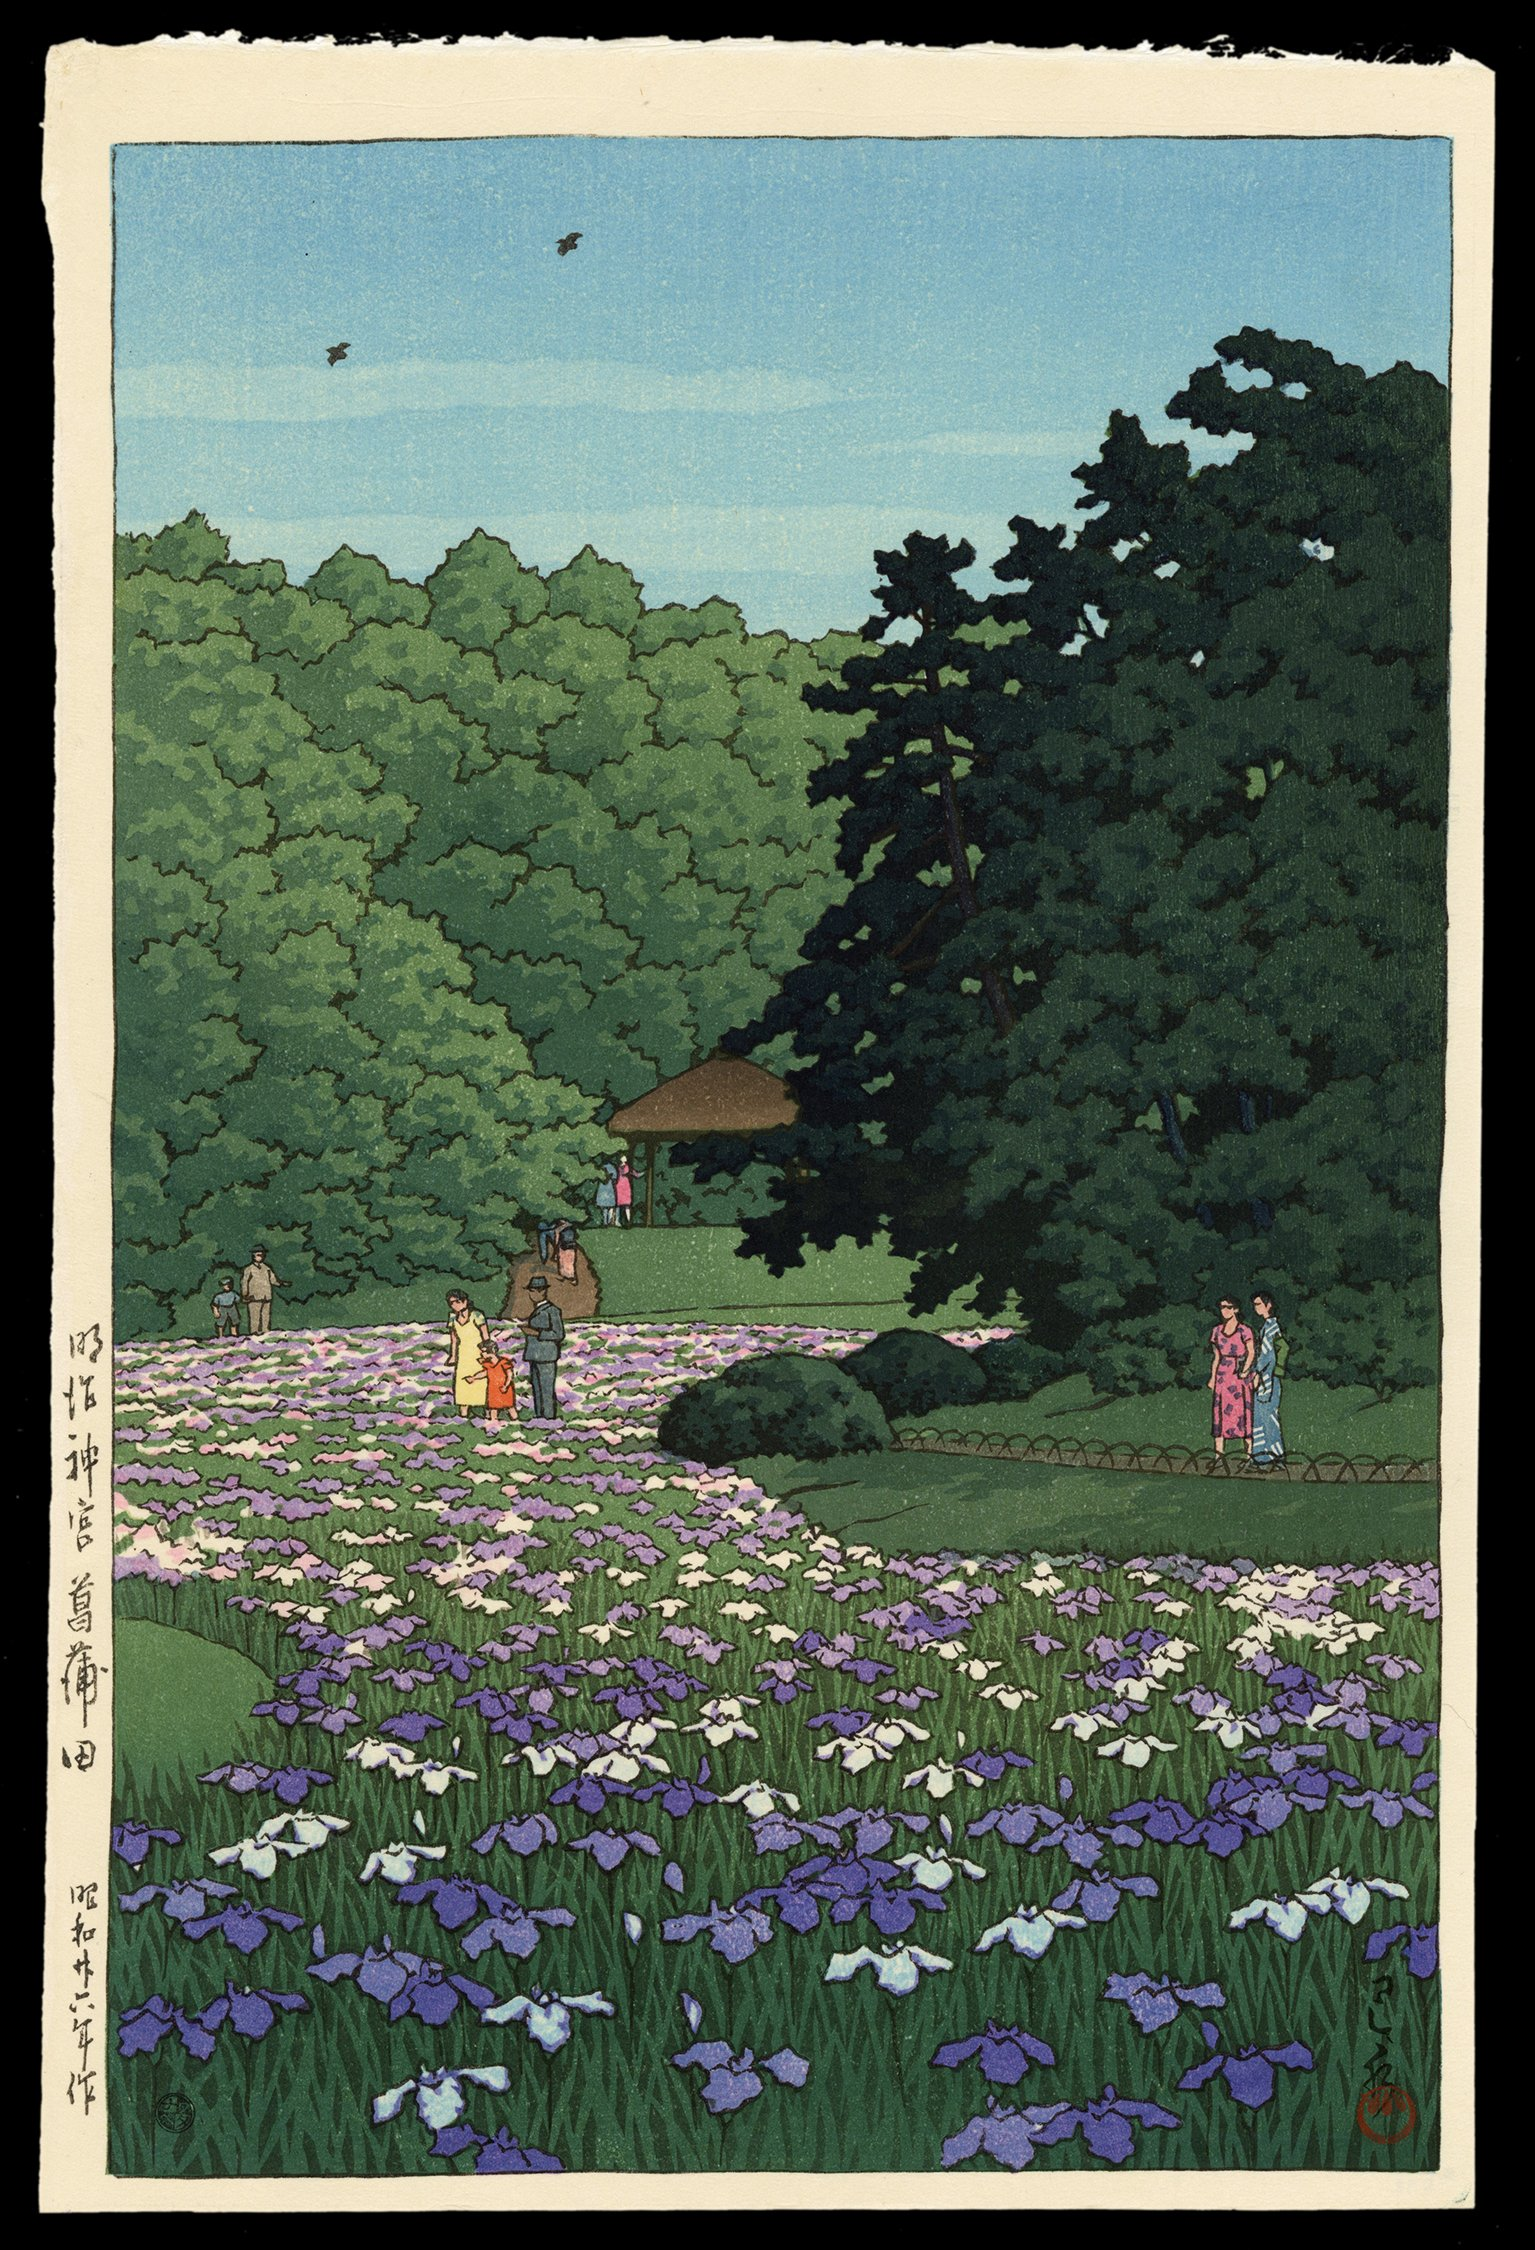
\includegraphics[width=0.5\linewidth]{irisgarden.jpg}
  \caption{Holzblock-Druck des Meiji-Schreines von Kawase Hasui (1883-1957)}
\end{center}
\end{figure}

Mit Erlaubnis der Behörden vermessen wir ein besonders hübsches Exemplar. Wir halten uns hier an die Reihenfolge der \textit{features} im Trainings-Datensatz:

\begin{lstlisting}[language=Python]
new_flower = [[5.1, 3.5, 12, 12]]
#              |    |    |   |
#              |    |    |   --- Länge des Blütenblatts in cm
#              |    |    ------- Breite des Blütenblatts in cm
#              |    ------------ Breite des Kelchblatts in cm
#              ----------------- Länge des Kelchblatts in cm
\end{lstlisting}

\begin{aufgabe}{3}
Diese Daten können wir aber nicht direkt so verwenden: Wir müssen alles, was wir mit den Trainingsdaten gemacht haben, auch mit den Daten für Vorhersagen machen. Was fehlt in diesem konkreten Fall noch?
\end{aufgabe}

Sobald wir die nötige Aufbereitung der Messdaten vorgenommen haben, können wir nun endlich unser Modell verwenden, um für komplett neue Daten eine Vorhersage zu treffen. In unserem Fall fragen wir unser Modell, zu welcher Iris-Art unser frisch vermessenes Exemplar zählt:

\begin{lstlisting}[language=Python]
DT.predict(new_flower_scaled)
\end{lstlisting}


\subsubsection*{Zusammenfassung}

In diesem Kapitel haben Sie gelernt, wie Sie mithilfe der Bibliothek \texttt{scikit-learn} maschinelles Lernen in Python praktisch umsetzen können. Anhand des bekannten Iris-Datensatzes haben Sie die typische Vorgehensweise kennengelernt:

\begin{itemize}
  \item \textbf{Importieren von Daten:} z. B. über \texttt{load\_iris(as\_frame=True)}
  \item \textbf{Zuweisung von \texttt{features} und \texttt{target}:} Eingabedaten (\texttt{X}) und Zielwerte (\texttt{y})
  \item \textbf{Aufteilen in Trainings- und Testdaten:} mit \texttt{train\_test\_split()}
  \item \textbf{Skalieren der Daten:} mit z.B. \texttt{MinMaxScaler()}
  \item \textbf{Modellwahl und Training:} mit \texttt{fit()}, z.B. \texttt{DecisionTreeClassifier()}
  \item \textbf{Evaluation des Modells:} mit \texttt{score()} oder Vergleich von \texttt{y\_test} und \texttt{y\_pred}
  \item \textbf{Modell speichern und laden:} mit \texttt{joblib.dump()} und \texttt{joblib.load()}
  \item \textbf{Vorhersagen treffen:} mit \texttt{predict()}
\end{itemize}

Die einheitliche Benennung (\texttt{fit()}, \texttt{predict()}, \texttt{score()}) erlaubt es, sehr einfach verschiedene ML-Algorithmen auszuprobieren ohne die gesamte Pipeline umstellen zu müssen. So können Sie Ihr Wissen über Entscheidungsbäume, lineare Regression oder \textit{k-means} direkt anwenden.





\end{lpu}



\subsection*{Didaktische Überlegungen}

In diesem Kapitel wurde bewusst auf eine grosse Anzahl entdeckender Aufgaben verzichtet. Der Grund dafür liegt in der Natur des behandelten Inhalts: Während viele frühere Kapitel dieser Unterrichtseinheit dazu einluden, Zusammenhänge und Strukturen selbständig zu entdecken (etwa bei Entscheidungsbäumen), handelt es sich hier um die praktische Umsetzung gelernter Konzepte in \texttt{python} und \texttt{scikit-learn}.

Die Umsetzung in Code ist in diesem Fall weniger ein Feld für offene Entdeckungen, sondern verlangt genaue Kenntnis spezifischer Befehle. Die APIs von \texttt{scikit-learn} sind zwar einheitlich und gut strukturiert, aber aufgrund des grossen Funktionsumfangs auch mit vielen möglichen Fehlerquellen verbunden. Selbst kleinere Unklarheiten bei den Argumenten einer Methode oder der Struktur der Eingabedaten führen schnell zu unverständlichen Fehlermeldungen oder nicht funktionierenden Vorhersagen.

Würde man die SuS in diesem Kapitel zu stark ``ausprobieren lassen'', wie es in konstruktivistisch geprägten Phasen sinnvoll ist, würde dies hier vor allem zu Frustration führen – insbesondere bei SuS, die noch nicht über viel Programmiererfahrung verfügen. Aus diesem Grund liegt der Fokus in diesem Abschnitt nicht auf Problemlösestrategien, sondern auf der \emph{sorgfältigen Übertragung Anwendung und Wiederholung} bereits erarbeiteter Inhalte. So kann Sicherheit im Umgang mit der Bibliothek aufgebaut werden, die sich später ausbauen liesse.


\subsection*{Musterlösungen}

\begin{aufgabe}{1}

Die Sitznachbarin hat sich entschieden, die alte Biologieprüfung auswendig zu lernen. Dabei hat sie sich nicht mit dem Stoff selbst, sondern mit dem \emph{genauen Wortlaut} der Aufgaben beschäftigt. Ihr Ziel war nicht, den Inhalt zu verstehen, sondern lediglich die exakten Fragen und Antworten zu memorieren.

Am Prüfungstag wurde sie jedoch überrascht: Die Lehrperson hat zwar ähnliche, aber nicht identische Fragen gestellt. Die zuvor auswendig gelernten Antworten helfen ihr jetzt kaum weiter. Wahrscheinlich wird sie Mühe haben, die neuen Fragen korrekt zu beantworten, weil sie den eigentlichen Stoff nie wirklich verstanden hat.

\textbf{Das ist ein klassisches Beispiel für \textit{overfitting}.} Im maschinellen Lernen bedeutet das, dass ein Modell die Trainingsdaten so gut ``gelernt'' hat, dass es nicht mehr auf neue, unbekannte Daten \textit{generalisieren} kann. Es hat nicht die \textit{Struktur} oder \textit{Logik} der Daten verstanden, sondern nur die Einzelbeispiele ``auswendig gelernt'' – wie die Schülerin die alte Prüfung.

\begin{itemize}
  \item \textbf{\textit{overfitting} anhand des Beispiels:}\\
  Die Sitznachbarin hat auswendig gelernt, statt zu verstehen. Das ist wie ein ML-Modell, das sich perfekt an die Trainingsdaten angepasst hat, aber bei neuen Daten versagt. Sie hat ein ``Modell'' erstellt, das nur für eine einzige Situation (die alte Prüfung) funktioniert. Sobald sich die Situation leicht ändert (neue Fragen), ist sie verloren.

  \item \textbf{Wie kann man \textit{overfitting} im ML vermeiden?}\\
  \begin{itemize}
    \item \textit{train-test split:} Man teilt die Daten in einen Trainings- und einen Testdatensatz. So kann überprüft werden, ob das Modell auch mit neuen Daten (Testdaten) gut funktioniert.
    \item \textit{Regulierung:} Manche Modelle erlauben Einstellungen, um extreme Anpassungen zu vermeiden (z.\,B. \texttt{max\_depth} bei Entscheidungsbäumen).
    \item \textit{Mehr Daten:} Wenn man viele unterschiedliche Trainingsbeispiele hat, ist es für das Modell schwieriger, ``auswendig zu lernen'' – und es lernt eher die allgemeinen Muster.
    \item \textit{cross validation:} Statt nur einmal zu testen, wird mehrfach mit unterschiedlichen Aufteilungen trainiert und getestet.
  \end{itemize}
\end{itemize}

\end{aufgabe}


\begin{aufgabe}{2}

\begin{enumerate}
  \item \textbf{\textit{one hot encoding} im Iris-Datensatz?}\\
  Im klassischen Iris-Datensatz ist das \texttt{y}-Array \textit{nicht} als \textit{one hot encoding} dargestellt, sondern als einfache Ganzzahlen:
  \begin{itemize}
    \item \texttt{0} steht für \textit{Iris setosa}
    \item \texttt{1} steht für \textit{Iris versicolor}
    \item \texttt{2} steht für \textit{Iris virginica}
  \end{itemize}
  Dies ist eine sogenannte \textit{integer encoded} Darstellung der Kategorien. Ein echtes \textit{one hot encoding} würde jede Kategorie mit einer einzigen 1 und sonst nur 0 dargestellt werden:
  \[
    \text{setosa} = [1, 0, 0],\quad
    \text{versicolor} = [0, 1, 0],\quad
    \text{virginica} = [0, 0, 1]
  \]

  \item \textbf{Sind die \texttt{X}-Werte im gleichen Wertebereich?}\\
  Nein. Die vier Spalten von \texttt{X} enthalten:
  \begin{itemize}
    \item \texttt{sepal length (cm)} – z. B. Werte um 5–7
    \item \texttt{sepal width (cm)} – z. B. 2–4
    \item \texttt{petal length (cm)} – z. B. 1–6.5
    \item \texttt{petal width (cm)} – z. B. 0.1–2.5
  \end{itemize}
  Die Werte liegen also in unterschiedlichen Bereichen und Skalen. Einige Spalten enthalten kleine Werte (z. B. \texttt{petal width}), andere deutlich grössere (\texttt{petal length}). Das könnte Algorithmen beeinflussen, die diese numerische Abstände berücksichtigen. Eine Skalierung (z. B. mit \texttt{MinMaxScaler} oder \texttt{StandardScaler}) könnte hier sinnvoll sein, um alle \textit{features} in denselben Bereich zu bringen und die Algorithmen nicht zu verzerren.
\end{enumerate}

\end{aufgabe}


\begin{aufgabe}{3}

Die neuen Daten (also neue Messungen der Blume) liegen im Rohformat vor – das heisst: Sie sind noch \textit{nicht skaliert}.

Da unser Modell jedoch mit skaliertem \texttt{X\_train} trainiert wurde, ist ein direkter Vergleich nicht möglich. Das Modell erwartet Eingabewerte im Bereich von $0$ bis $1$, nicht in Zentimetern. Wir müssen also auch die neuen Daten zuerst durch den \texttt{Scaler} schicken, mit dem wir die Trainingsdaten skaliert haben:

\begin{lstlisting}[language=Python]
new_flower_scaled = scaler.transform(new_flower)
\end{lstlisting}

Erst danach dürfen wir sie für eine Vorhersage verwenden:

\begin{lstlisting}[language=Python]
prediction = model.predict(new_flower_scaled)
\end{lstlisting}

Bei neuen Eingabedaten müssen immer dieselben \textit{preprocessing}-Schritte durchgeführt werden wie bei den Trainingsdaten – sonst ``versteht'' das Modell die Zahlen nicht im richtigen Kontext.

\end{aufgabe}


\section{Wissensfestigung}
\label{sec:wissensfestigung}

Im Anhang befinden sich die Dateien \texttt{files/LA\_1651} und \texttt{files/LA\_1651\_L} (die dazugehörige Musterlösung). Sie sind Notizbücher, welche als \textbf{Abschlussübung} für die SuS eingesetzt werden sollten: Sie ist herausfordernd, aber verlangt von den SuS einen echten Wissenstransfer, da sie hier das im letzten Kapitel der LPU Gelernte auf einen neuen Datensatz (nämlich den Titanic-Datensatz) anwenden. Es ist ein vollständiges, (Miniatur-)ML-Projekt von der Datenaufbereitung bis zur Vorhersage, welche die SuS selbständig bearbeiten können. Das Notizbuch ist dabei so angelegt, dass schwierige Teile vorgegeben sind, aber diejenigen Stellen im Code, welche die SuS selbständig aus der Bearbeitung dieser LPU ableiten können, freigelassen sind. 


Eine weitere Möglichkeit zur Wissensfestigung oder -Prüfung wäre ein ``Vokabel-Test'', bei welchem die SuS das während der LPU erstellte, persönliche Glossar verwenden dürfen.

In dieser Phase empfiehlt es sich, das Rollenverständnis der SuS zu verschieben: Vom ``Nachvollziehen'' einzelner Anweisungen hin zum ``Selbststrukturieren'' ganzer Projekte. Die festigende Wirkung tritt nicht allein durch Wiederholung ein, sondern durch sinnvolle und zunehmend selbstständige Anwendung – gestützt durch die direkte Rückmeldung der Notizbücher und Vergleich mit der Musterlösung von \texttt{LA\_1651}.

\newpage
\section{Ausblick}
\label{sec:abschluss}

Diese LPU gibt einen Einblick in die wichtigsten, grundlegenden Algorithmen und vermittelt den SuS ein theoretisches und praktisches Verständnis derer. Sie bietet eine optimale Grundlage, um kompliziertere ML-Algorithmen einzuführen, wie bspw. das \textit{Perzeptron}. Aufbauend darauf könnte dann der Begriff des \textit{mehrschichtiges Lernen} lernen eingeführt werden.

Parallel dazu gilt es sicher auch die Evaluations-Metriken, welche lediglich im letzten Kapitel der LPU und bei der Besprechung des MSE gestreift wurden, zu vertiefen. 

\end{document}
